\chapter{Concepts} \label{sec:Concepts}

\todoall{Description of elements should follow this structure: What is it for? What does it do? Examples in concrete syntax + explanation}

\section*{Old stuff from rejected paper}
In this section, we will briefly introduce story diagrams and their current features. 
Story diagrams combine
UML activity diagrams and graph transformations by embedding graph replacement rules into the activities.
This allows the activities in Figure \ref{fig:transformationOverview} to be specified formally by graph replacements while preserving the general control flow structure of the example transformation.

In terms of the classification of model transformations proposed by Czarnecki and Helsen~\cite{Czarnecki06}, story diagrams are an endogenous, in-place transformation language.
It has both declarative (pattern matching) and operational elements (specification of control flow):
Its control flow allows a deterministic selection of the graph replacement rules to be applied, with a (non-deterministic) pattern matching in the graph replacement rules.
It can also be used for inter-model transformations to create a new target model from a given source model, as seen in the example given in this paper. 
In order to execute story diagrams, code generation \cite{GBD07} and interpretation \cite{GHS09} are supported.

In the following, we will describe the graph transformations, the so-called story patterns, in Section~\ref{sec:StoryPatterns}.
Afterwards, we will explain how control flow can be modeled by using elements from activity diagrams in Section~\ref{sec:StoryDiagrams}.

	\section{Story Diagrams and Story Patterns in a Nutshell (Dietrich \& Jan)} \label{sec:Overview}

%- model-driven software development, raise abstraction level and use models instead of code as the key artifact
%- specify structure and behavior of the software under development, make the models runnable/executable
%- UML offers notations for description of software structure and development, esp. class and activity diagrams
%- activity diagrams are too informal to be automatically executed (natural language used)
%- we replaced the informal activity descriptions with formal descriptions of operations on object structures and developed a new formal language called story diagrams

%- story diagrams are special UML activity diagrams
%- developed to formalize the description of a software's behavior (UML activity diagrams usually use informal textual descriptions of the tasks to be performed)
%- motivation: complete specification of a software, structure and behavior, i.e. make the software specification executable (code generation and interpretation)

In model-driven software development, a software model is the key artifact of the development.
It describes the software's structure as well as its behavior and 
can be translated into executable source code or be interpreted to be executed.
The UML offers notations for the description of the software structure and behavior,
besides others class diagrams and activity diagrams.
However, since UML activity diagrams use natural language in the activity nodes to describe the particular activities, they are not automatically executable.
Thus, a formal behavioral specification is needed.
For that purpose, \emph{story diagrams} have been developed \cite{FNTZ00,Zun01}.
They are based on UML 1.5 activity diagrams \cite{UML1.5} and replace the natural language with a formal language to specify behavior
and, thus, can be automatically executed.

In terms of the classification of model transformation languages proposed by Czarnecki and Helsen \cite{Czarnecki06},
story diagrams are an endogenous, in-place transformation language (see also Section~\ref{sec:foundations:typedAttrGTS}).

%- motivation: (formally) describe modifications of object structures for object-oriented software systems
%- use a graphical notation to specify operations on object structures (object structure modifications), OO world
%- each operation describes a modification of a given object structure, basically the modifactions are creations and removals of objects and their interconnections
%- graphically describe the object structure to be modified, mark the elements to be created and those to be removed

Story diagrams describe the control flow similar to UML activity diagrams by means of activity nodes and activity edges.
The behavior of each activity node is described using a graph transformation language called \emph{story patterns}.
Each activity node embeds one story pattern.
A story pattern uses a graphical notation to specify modifications of object structures in object-oriented software systems.
The modifications are basically creations and removals of objects and their interconnections (links).

%- motivation: use an appropriate, familiar, and simple notation for object structure modifications; we use a notation similar to UML object diagrams
%- motivation: declaratively describe the operations in activity nodes, thus, reduce complexity (avoid describing how to perform the operations)
%- motivation: keep determinism to a certain extent to specify the conditions for and the order of object structure modifications

Using a simple and familiar notation, story patterns are similar to UML object diagrams (see the embedded story pattern in Figure~\ref{fig:SDExampleStoryDiagram}).
A story pattern represents an object structure that is to be modified.
It includes annotations specifying which objects and links are to be removed and created.
Story patterns are a declarative language since they only specify what to remove and create but not how to do it and in which order.
This way, the complexity of the behavioral specifications is reduced.
In contrast to the deterministic control flow specified by activity nodes and edges which determine the order of story pattern executions,
the order of creations and deletions specified by a story pattern is non-deterministic.

%- motivation: base the specification on a well-known formalism (for execution and analyses)
%- story diagrams use graph transformations in their activity nodes (well-known formalism, exhaust the given theories for analyses and execution)

Story patterns are based on the well-known formalism of \emph{graph transformation systems} and the corresponding theory \cite{Roz97}.
Thus, precise analyses of the operations described by story patterns are possible,
e.g., it can be checked if certain properties of the object structure to be modified remain after the structure's modification \cite{Sch06,Mey09}.

%- given a so called host graph (an object structure or model), story diagrams describe the graph's modifications by means of creating or removing nodes and edges (objects and links)
%- the host graph, in our case, is a typed attributed graph, i.e. we have a graph to be modified (object structure, token model) and a corresponding type graph (type model or meta-model) describing the types and properties of the objects in our host graph
%- a graph transformation is executed by identifying a subgraph in the host graph which corresponds to the graph specified in the transformation (matching, subgraph isomorphism), removing nodes and links that are marked to be removed, and creating new nodes and links that are marked to be created

A story pattern specifies a graph transformation \cite{Roz97}.
Given a so-called \emph{host graph}, i.e.\ the graph to be modified, a graph transformation removes and creates nodes and edges in the given host graph.
The host graph is a typed attributed graph, i.e.\ there is a \emph{type graph} determining the types and attributes of the nodes.
A graph transformation is executed on a host graph by identifying a subgraph in the host graph that is similar to the one specified in the graph transformation
and then removing and adding the specified nodes and edges.
The identification of the subgraph for modification is called \emph{graph matching} and includes the \emph{subgraph isomorphism} problem
(see Chapter~\ref{sec:foundations} for more details).

In case of story patterns, the host graph is the object structure or model to be modified, i.e.\ the run-time data of the executed software.
Thus, we call the host graph's nodes and edges \emph{objects} and \emph{links}
while the host graph itself is called \emph{instance model}\footnote{Thomas K\"{u}hne calls it \emph{token model} \cite{Kue06}.} (or simply model) in the remainder of the report.
The type graph is a set of classes and their relations which define all potential instance models at run-time.
These classes and relations constitute a so-called \emph{type model} or the \emph{metamodel} \cite{Kue06} of the language used to describe instance models.
Furthermore, we call the nodes and edges in story patterns \emph{object variables} and \emph{link variables}
since these represent and are matched to objects and links in the instance model.
The types of these variables are determined by types in a type model which is required to specify story patterns.

\begin{figure}[htb]
	\centering
  \begin{minipage}[t]{.4\textwidth}
    \centering
    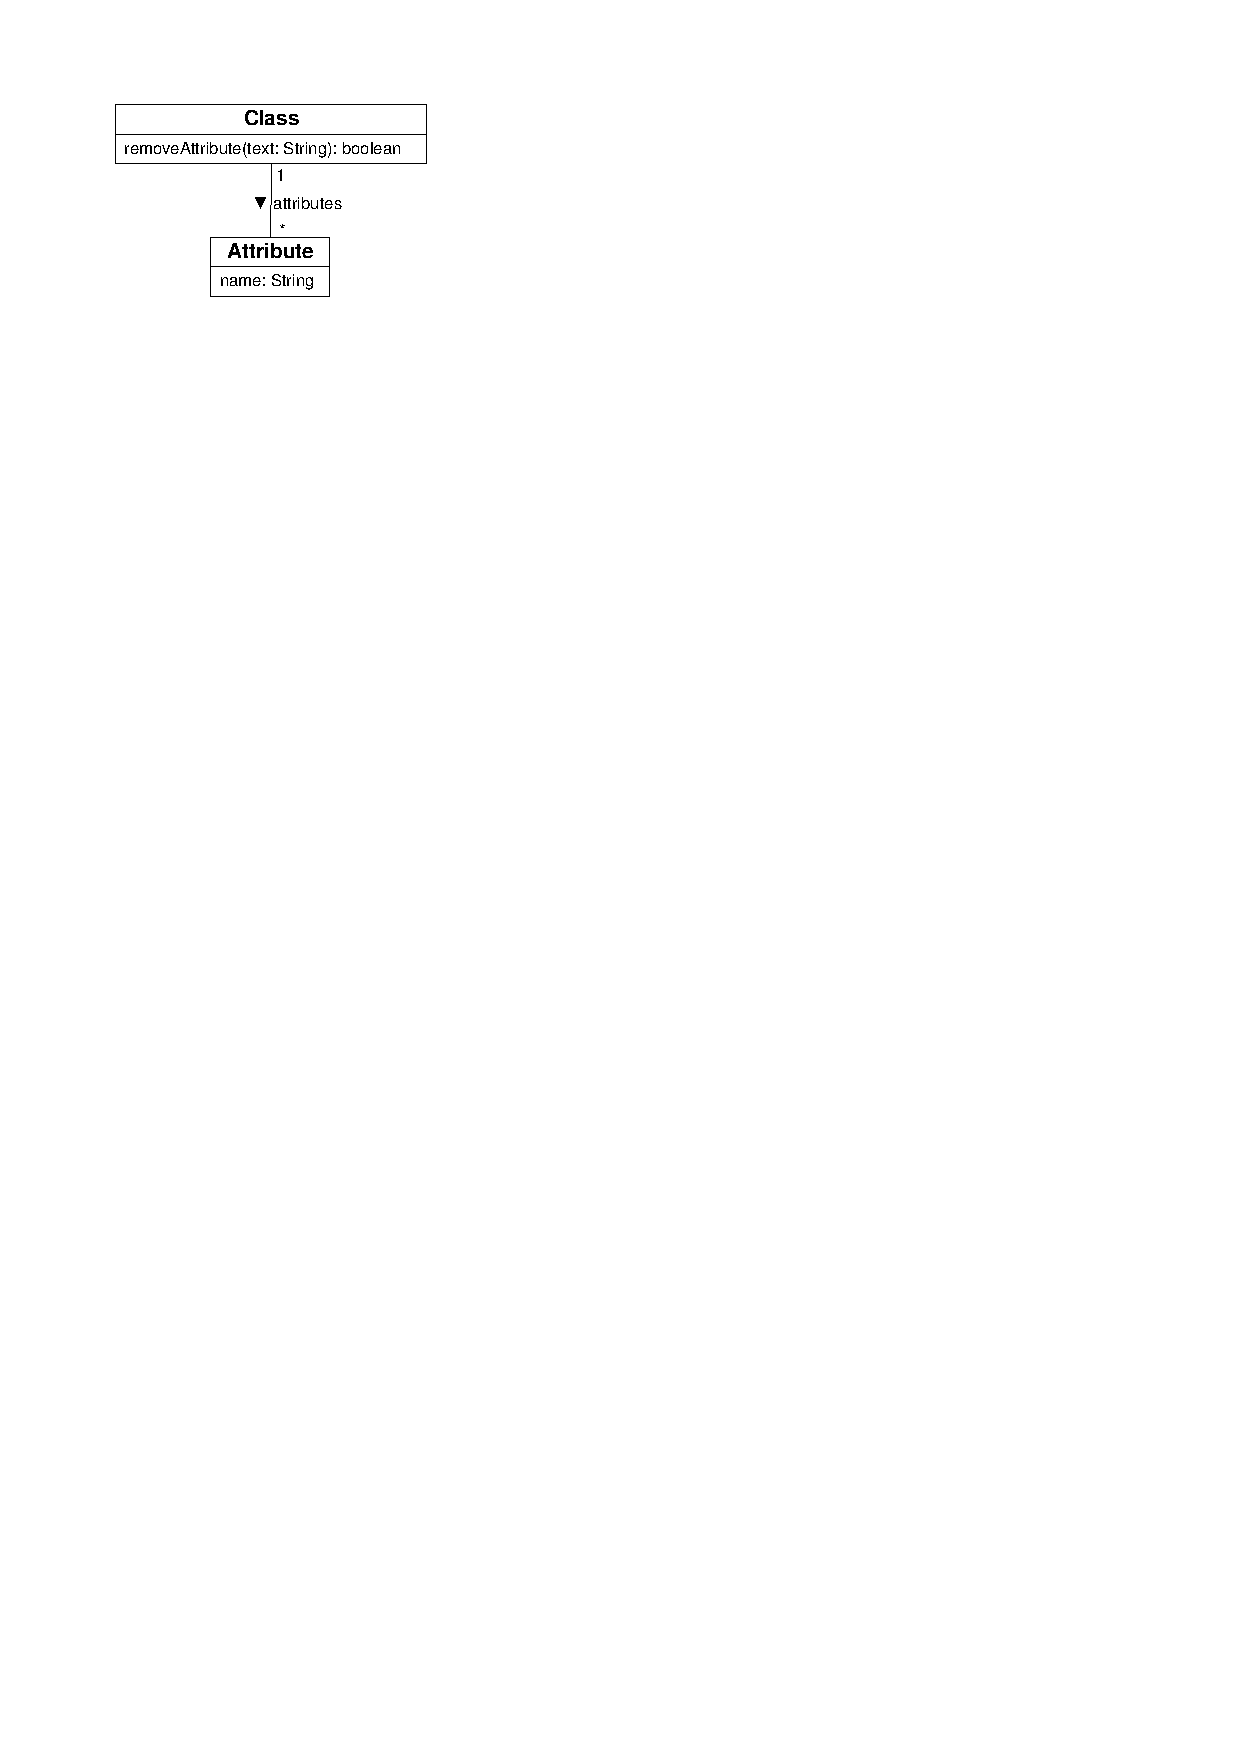
\includegraphics[scale=1]{SimpleSDRemoveAttributeClassDiagram} 
    \caption{Exemplary Type Model}
    \label{fig:SDExampleClassDiagram}
  \end{minipage}%
  \hfill
  \begin{minipage}[t]{.55\textwidth}
    \centering
    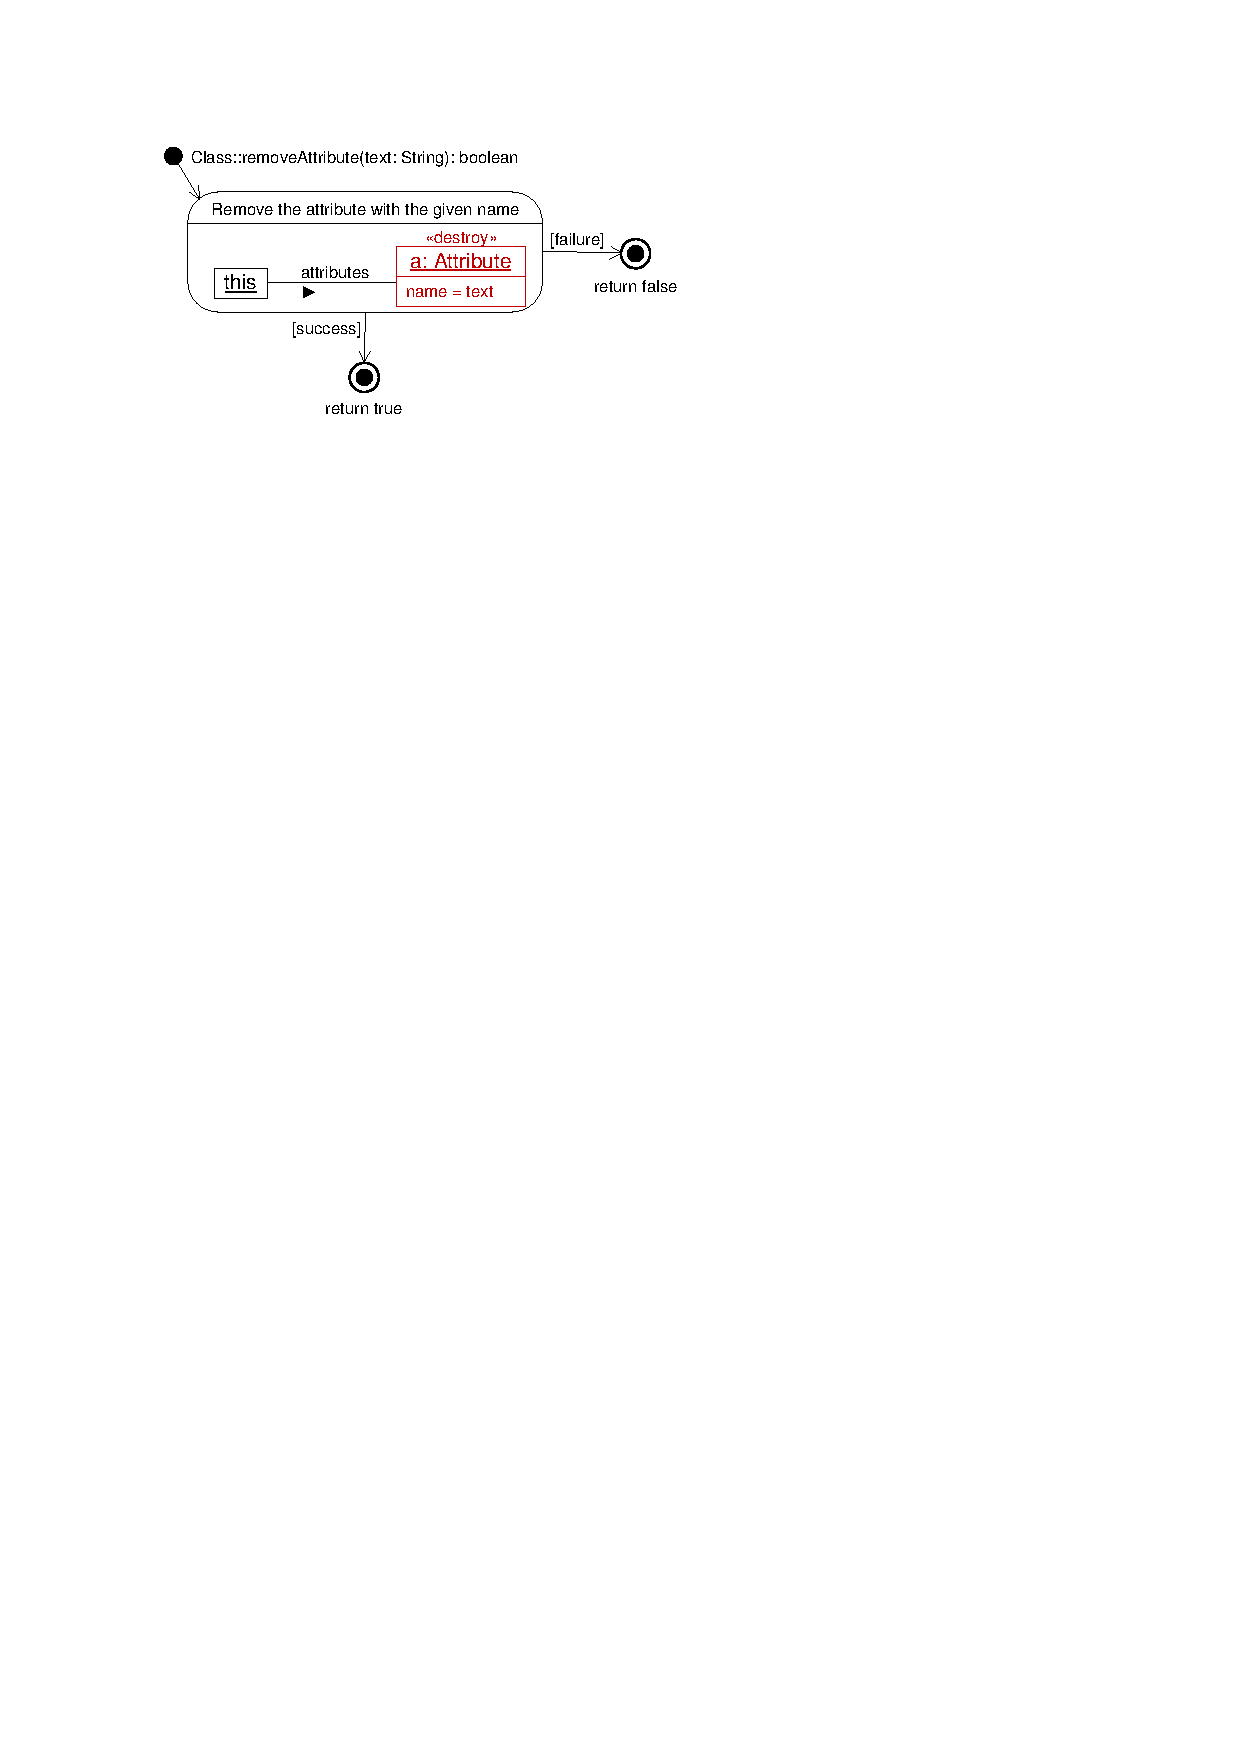
\includegraphics[scale=1]{SimpleSDRemoveAttribute}
    \caption{Exemplary Story Diagram}
    \label{fig:SDExampleStoryDiagram}
  \end{minipage}
\end{figure}

For example, the class diagram in Figure~\ref{fig:SDExampleClassDiagram} defines the types \fe{Class} and \fe{Attribute} as well as their relations, attributes, and operations.
The corresponding story diagram in Figure~\ref{fig:SDExampleStoryDiagram} defines the behavior of the \fe{removeAttribute} method defined in the class diagram.
Here, the story diagram specifies that a class's attribute with the name given by the parameter \fe{text} is to be found in the instance model and in case of success this attribute is to be removed (\destroy).

In summary, a story diagram is a special, formally defined UML activity diagram
that embeds graph transformations, so-called story patterns, in its activity nodes
to precisely describe run-time behavior by means of graph transformations.

%\subsection{Application scenarios (?)} \label{sec:Applications}

	\section{Story Patterns} 
\label{sec:StoryPatterns}

In this section, we introduce story patterns in more detail.
We start by giving the general idea of story patterns in Section \ref{sec:StoryPatterns:storyPattern}.
Thereafter, we describe the basic concepts of story patterns, namely object variables, link variables,
and their respective binding semantics in Sections \ref{sec:StoryPatterns:objects} to \ref{sec:StoryPatterns:binding}.
Finally, we show the use of object attributes in a story pattern in Section \ref{sec:StoryPatterns:attributes}.


\subsection{General Idea}
\label{sec:StoryPatterns:storyPattern}

Story patterns are typed attributed graph transformation rules with inheritance on object types (cf. Section~\ref{sec:foundations:typedAttrGTS}) that can be embedded into an activity node of a story diagram (cf. Section~\ref{sec:StoryDiagrams}).
 By using a type model as introduced in Section~\ref{sec:foundations:typedAttrGTS}, story patterns enable polymorphism for matching object and link variables.
This allows for specifying graph replacement rules for object-oriented models.

Object and link variables are matched to the objects and links of the instance model. 
In contrast to typed attributed graph transformations, story patterns explicitly require to use isomorphic matchings, i.e., two object variables of a story pattern may not be matched to the same object of the instance model.

For enabling a concise notation of the graph transformation, story patterns apply a short-hand notation depicting the left-hand side (LHS) and the right-hand side (RHS) in a single, annotated graph using stereotypes.
In the short-hand notation, we use binding operators for defining the LHS and the RHS. Object and link variables representing objects and links not to be changed by the story pattern carry no stereotype. 
Object and link variables representing objects to be created (or deleted) are annotated with \create (or  \destroy, respectively). 
Consequently, the LHS consists of all object and link variables that carry no stereotype or stereotype \destroy. The RHS consists of all object and link variables that carry no stereotype or the stereotype \create.
The deletion of objects and links follows the single-pushout approach (cf.\ Section~\ref{sec:foundations:simpleGTS}).

Figure \ref{fig:simpleStoryPattern} shows an example of a single story pattern that redirects a method call from an old method to a new method.
\begin{figure}[htb]
  \centering
  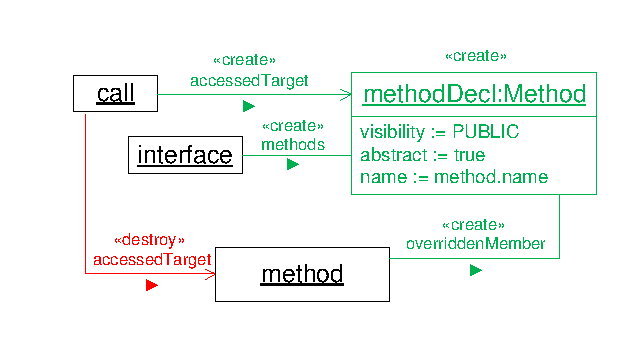
\includegraphics[scale=1.0]{figures/SimpleStoryPattern}
  \caption{Example of a Story Pattern}
  \label{fig:simpleStoryPattern}
\end{figure}
In the example, the object variables \fe{parentClass}, \fe{oldMethod}, and \fe{newMethod} are bound variables, i.e., they already refer to objects of the instance model (cf. Section \ref{sec:StoryPatterns:binding:states}).
The object variables \fe{anyMethod} and \fe{c} are unbound. 
When applying the story pattern, first a match for \fe{anyMethod} and \fe{c} is searched in the instance graph. 
A possible match will be any method in \fe{parentClass} which contains a call to \fe{oldMethod}. 
If the matching is successful, the link from \fe{c} to \fe{oldMethod} will be deleted and the link from \fe{c} to \fe{newMethod} will be created.

In the concrete syntax of story patterns, the object and link variables representing objects and links not to be modified by the story pattern are visualized in black. 
Object and link variables representing objects and links to be destroyed are annotated with \destroy and visualized in red. 
Object and link variables representing objects and links to be created are annotated with \create and visualized in green. 
An unbound object variable is labeled with its name and the name of the corresponding type. 
For bound object variables, we omit the name of the type (e.g., \fe{parentClass} in Figure~\ref{fig:simpleStoryPattern}).

In general, the matching process is executed as a three step process:
first, a matching is searched which uses the bound variables of the story pattern as a starting point. The matching associates objects and links of the instance model to all object and link variables of the story pattern. 
The matching is performed as defined for typed attributed graph transformations and considers all object and link variables of the LHS.
If a matching can be obtained, the story pattern is applicable and the execution proceeds. 
\tododt{What happens if the modification operations are contradictory (see Section~\ref{sec:DecisionNodesEtc})?}
Otherwise the execution of the story pattern is aborted.
In the second step, all objects and links matched to object and link variables annotated with \destroy are deleted. 
Finally, objects and links are created in the instance model for all variables annotated with \create.

Story patterns aim to reduce the computational complexity of the matching process (cf. Section~\ref{sec:foundations:simpleGTS}) by using bound variables.
We require at least one bound object variable in each story pattern which is used as a starting point for the matching process.


\subsection{Objects and Object Variables}
\label{sec:StoryPatterns:objects}

Object variables in a story pattern represent the objects in an instance model to be matched.
The variables are uniquely identified by their name.
The objects are instances of classes of the underlying type model (cf.
Section \ref{sec:foundations:typedAttrGTS}). Thus, the object variables are typed by classes from this model.

The story pattern in Figure \ref{fig:simpleStoryPattern} contains five
object variables with the names \fe{parentClass}, \fe{oldMethod}, \fe{anyMethod}, \fe{c} and
\fe{newMethod}. 
The type of an object variable is only visualized if the
variable is unbound or maybe bound (cf.\ Section
\ref{sec:StoryPatterns:binding:states}). For example, the object variable \fe{anyMethod} has the type \fe{Method}.

Object variables have binding states, binding operators and binding semantics which are described in Section  \ref{sec:StoryPatterns:binding}.


\ext %--- Comment this line to include primitive variables into the document
{
\todomcp{Primitive Variables: concrete syntax like
object variables; binding expressions for initialization, see figure
\ref{fig:primitiveVariable}; primitive variables are typed over EDataType; they
exist to the end of the Activity}

\begin{figure}[htb]
  \centering
  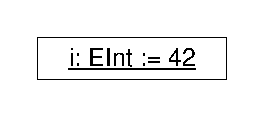
\includegraphics[scale=0.6]{figures/PrimitiveVariable}
  \caption{Primitive variable with value assignment}
  \label{fig:primitiveVariable}
\end{figure}

\todomcp{Links to primitive variables: special LinkVariable, typed over
EStructuralFeature}
}%------ End of primitive variables section



\subsection{Links and Link Variables}
\label{sec:StoryPatterns:links}

Link variables represent connections between objects and are used to connect
different object variables.
A link variable is typed over a reference of the underlying type graph.
\tododt{The typing should be described more precisely.
The link variable is typed over one or two corresponding \fe{EReferences} that conceptually represent a uni-directional or bi-directional association.}

Like object variables, link variables also have binding
operators and binding semantics (cf. Section \ref{sec:StoryPatterns:binding}), but no binding state.




\subsection{Binding of Variables}
\label{sec:StoryPatterns:binding}

Object variables have binding states (unbound, bound, maybe
bound), binding semantics (mandatory, negative, optional), and binding operators
(check only, create, destroy). Link variables have binding
operators and binding semantics.
Their meaning is described in the following. 


\subsubsection{Binding States}
\label{sec:StoryPatterns:binding:states}

An object variable or a link variable can be declared as \emph{bound}, \emph{unbound}, or
\emph{maybe bound} (i.e., it is unknown if the variable is bound or not). This is
defined by its binding state. An unbound variable is matched during the
execution of the containing story pattern. 
A bound variable must have been matched previously. 
For a variable that is specified as maybe bound, a new match will only be
determined if it has not been bound before. 
Otherwise it will be treated as a bound variable.
This is useful, if the same pattern should be used in different contexts, i.e., the bound variable of the pattern differs depending on the context but otherwise the patterns are identical.
Without maybe bound variables, different patterns would have to be modeled that only differ in which variable is the bound variable of the pattern.
With maybe bound variables, all variables can be set to maybe bound and the caller specifies a binding for one of them depending on the context.
%\todomcp{explain why maybe bound is necessary}

Unbound object variables are visualized with an underlined label of the form
``name: Type'' (cf. Figure \ref{fig:bindingStatesOverview} a)).
For bound object variables the type is hidden, as depicted
in Figure \ref{fig:bindingStatesOverview} b).
Maybe bound object variables are represented like unbound object variables, but
are marked by a question mark after the name (cf.\ Figure
\ref{fig:bindingStatesOverview} c)).

In a valid story pattern, each connected component\footnote{With
``connected component'' we mean a subgraph in which each object variable is
reachable from at least one bound object variable via directed link variables.}
must contain at least one bound object variable or created variables only. This
is necessary to avoid a search over the whole underlying instance model which requires a long runtime in most cases (cf. Section~\ref{sec:StoryPatterns:storyPattern}).

\begin{figure}[htb]
  \centering
  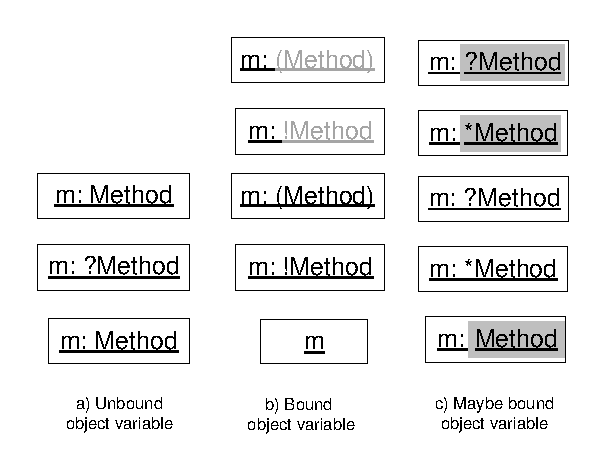
\includegraphics[scale=1.2]{figures/BindingStatesOverview}
  \caption{Binding States for Object Variables}
  \label{fig:bindingStatesOverview}
\end{figure}

\subsubsection{Binding Semantics}
\label{sec:StoryPatterns:binding:semantics}
Object variables and link variables have binding semantics that
determine if a variable is mandatory, negative or optional.
A match for mandatory variables must exist in the given instance model, otherwise
the pattern matching fails. 
In contrast, negative variables constitute so-called negative application
conditions (NACs) and must not exist in the instance model. If a variable defined as
negative can be matched during the execution of the story pattern, the pattern matching
fails. Matches for optional variables may exist. An optional variable will be
bound if possible, but the story pattern may also be matched
successfully otherwise.

Negative object variables are visualized crossed-out (cf. Figure
\ref{fig:bindingSemanticsOverview} b)) and optional object variables are
visualized with a dashed border (cf.\ Figure \ref{fig:bindingSemanticsOverview} c)).
The same holds for negative and optional link variables (cf. Figure
\ref{fig:bindingSemanticsOverview} e) and f)).

Negative as well as optional object and link variables are not part of a
connected component.
This means, the graph has to be still connected when ignoring optional and negative
parts. However, optional and negative object variables must be reachable from a connected component. 
Consequently, regarding the rule that each connected component must
contain at least one bound object variable (cf.\ Section
\ref{sec:StoryPatterns:binding:states}), there are situations in which the
use of negative or optional object variables is not allowed. 
Figure \ref{fig:negativeObjects} shows these situations. 
Case a) is allowed but case b) is not because, in the latter case,
the graph without the negative and optional elements is not a connected component anymore.
Case c) is allowed because the object
variables \fe{a} and \fe{c} are bound which means that each connected component has at least one bound object variable.
Accordingly, case d) is allowed, too, because \fe{a} and \fe{b} are both
bound. Case e) is not allowed while Case f) is.
Case g) is not allowed because the semantics is the same as in Case a) due to the single-pushout approach of story patterns.

Similar to the application of negative object
variables, Figure \ref{fig:optionalObjects} shows some examples for the application of optional object variables. 
While case a) is allowed, case b) is not allowed because in this case the
shown graph is not connected anymore. However, case c) and d) are allowed
because each connected component contains at least one bound object variable.
Cases e) and f) are also allowed.

\begin{figure}[htb]
  \centering
  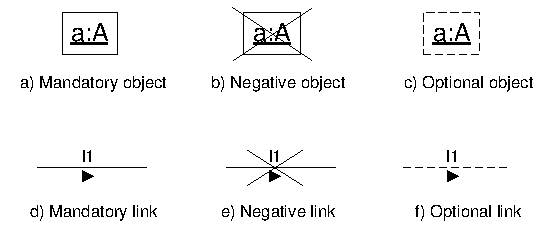
\includegraphics[scale=1.2]{figures/BindingSemanticsOverview}
  \caption{Binding Semantics for Object and Link Variables}
  \label{fig:bindingSemanticsOverview}
\end{figure}

\begin{figure}[htb]
  \centering
  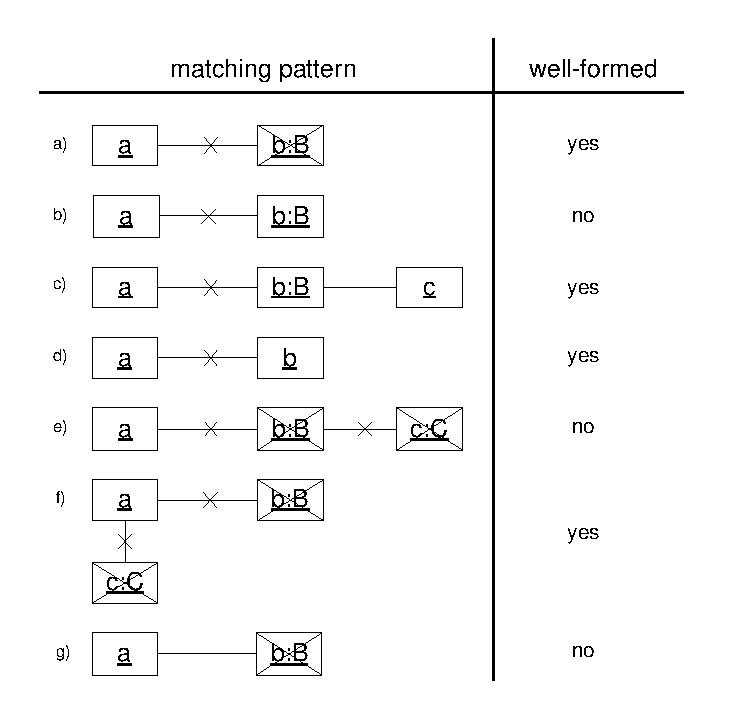
\includegraphics[scale=1]{figures/negativeObjects}
  \caption{Negative Application Conditions}
  \label{fig:negativeObjects}
\end{figure}

\begin{figure}[htb]
  \centering
  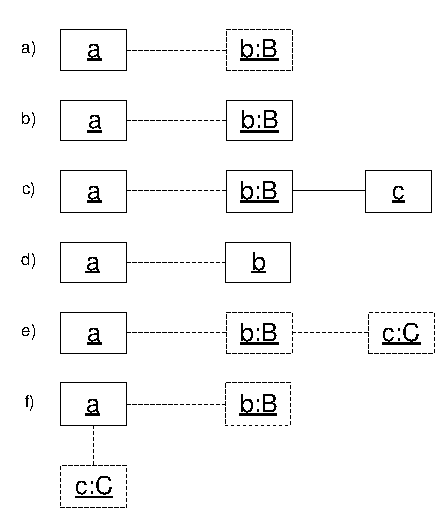
\includegraphics[scale=1]{figures/optionalObjects}
  \caption{Optional Object and Link Variables}
  \label{fig:optionalObjects}
\end{figure}


\subsubsection{Binding Operators}
\label{sec:StoryPatterns:binding:operators}

Binding operators define whether an object or link is to be created, deleted,
or just matched in the instance model.
After all elements that are defined to be deleted or just matched have been
matched, the model is modified by deleting and creating the elements as
defined (see Section~\ref{sec:StoryPatterns:storyPattern}).

It may happen that a matching is successful but that the specified creation is infeasible.
For instance, constraints imposed upon the elements to be created may be contradictory (see Section~\ref{sec:StoryPatterns:linkConstraints:orderConstraint}).
Of course, it is not sensible to specify such constraints but it cannot always be checked statically if constraints are contradictory or not.
If such a situation is detected at execution time, the execution of the story diagram is aborted.

Objects and links to be created are marked with the
stereotype \create (cf.\ Figure \ref{fig:bindingOperatorsOverview} b) and e)) and objects and links
to be deleted are marked with the stereotype \destroy (cf.\ Figure
\ref{fig:bindingOperatorsOverview} c) and f)).

\begin{figure}[htb]
  \centering
  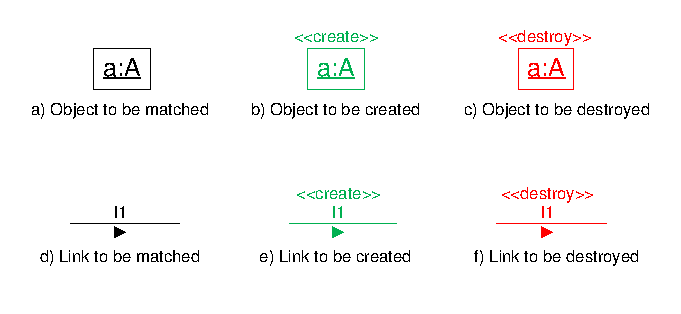
\includegraphics[scale=1.2]{figures/BindingOperatorsOverview}
  \caption{Binding Operators for Object and Link Variables}
  \label{fig:bindingOperatorsOverview}
\end{figure}

Since no objects and links exist for variables marked with \create, they also do not belong to a connected component (like
negative or optional variables).


\subsubsection{Feasible Binding Combinations}

Binding states, binding semantics and binding operators can be
arbitrarily combined, but only certain combinations are feasible. 
Table \ref{tab:bindingCombinations} lists all feasible binding combinations for
object variables. As shown there, bound and maybe bound object variables must not have negative
or optional binding semantics. As well, the combination of the binding states
bound or maybe bound and the binding operator create is not allowed.

% Table generated by Excel2LaTeX from sheet 'Tabelle1'
\begin{table}[htbp]
  \centering
  \caption{Feasible Combinations of Binding States, Binding Semantics, and
  Binding Operators for Object Variables}
    \begin{tabular}{|r|r|r|r|}
    \hline
    \textbf{Binding State} & \textbf{Binding Semantics} & \textbf{Binding
    Operator} & \textbf{Feasible} \\
    \hline
    UNBOUND & MANDATORY & CHECK\_ONLY & yes \\
    UNBOUND & MANDATORY & CREATE & yes \\
    UNBOUND & MANDATORY & DESTROY & yes \\
    UNBOUND & NEGATIVE & CHECK\_ONLY & yes \\
    UNBOUND & NEGATIVE & CREATE & no \\
    UNBOUND & NEGATIVE & DESTROY & no \\
    UNBOUND & OPTIONAL & CHECK\_ONLY & yes \\
    UNBOUND & OPTIONAL & CREATE & yes \\
    UNBOUND & OPTIONAL & DESTROY & yes \\
    \hline
    BOUND & MANDATORY & CHECK\_ONLY & yes \\
    BOUND & MANDATORY & CREATE & no \\
    BOUND & MANDATORY & DESTROY & yes \\
    BOUND & NEGATIVE & CHECK\_ONLY & no \\
    BOUND & NEGATIVE & CREATE & no \\
    BOUND & NEGATIVE & DESTROY & no \\
    BOUND & OPTIONAL & CHECK\_ONLY & no \\
    BOUND & OPTIONAL & CREATE & no \\
    BOUND & OPTIONAL & DESTROY & no \\
    \hline
    MAYBE\_BOUND & MANDATORY & CHECK\_ONLY & yes \\
    MAYBE\_BOUND & MANDATORY & CREATE & no \\
    MAYBE\_BOUND & MANDATORY & DESTROY & yes \\
    MAYBE\_BOUND & NEGATIVE & CHECK\_ONLY & no \\
    MAYBE\_BOUND & NEGATIVE & CREATE & no \\
    MAYBE\_BOUND & NEGATIVE & DESTROY & no \\
    MAYBE\_BOUND & OPTIONAL & CHECK\_ONLY & no \\
    MAYBE\_BOUND & OPTIONAL & CREATE & no \\
    MAYBE\_BOUND & OPTIONAL & DESTROY & no \\
    \hline
    \end{tabular}%
  \label{tab:bindingCombinations}%
\end{table}%

%\todomcp{see albert's habil for example for optional-create}

%\todomcp{table for object set variables?}

\begin{table}[htbp]
  \centering
  \caption{Feasible Combinations of Binding Semantics and
  Binding Operators for Link Variables}
    \begin{tabular}{|r|r|r|}
    \hline
    \textbf{Binding Semantics} & \textbf{Binding
    Operator} & \textbf{Feasible} \\
    \hline
    MANDATORY & CHECK\_ONLY & yes \\
    MANDATORY & CREATE & yes \\
    MANDATORY & DESTROY & yes \\
    NEGATIVE & CHECK\_ONLY & yes \\
    NEGATIVE & CREATE & no \\
    NEGATIVE & DESTROY & no \\
    OPTIONAL & CHECK\_ONLY & yes \\
    OPTIONAL & CREATE & yes \\
    OPTIONAL & DESTROY & yes \\
    \hline
    \end{tabular}%
  \label{tab:bindingCombinations_links}%
\end{table}%

The feasible combinations of binding semantics and binding operators for link
variables are given in Table \ref{tab:bindingCombinations_links}. Link variables
have no binding state.


\subsection{Using Object Attributes}
\label{sec:StoryPatterns:attributes}

The objects of our instance model carry attributes. 
During the application of a story pattern, these attributes can be used twofold. 
First, attribute constraints can be specified to restrict the attribute values to a certain range, thereby restricting the possible matches of a story pattern. 
Second, attribute values can be changed during the graph rewriting step after a successful matching.

We use \emph{attribute constraints} to restrict the matching of object variables to objects of the instance model that have specific attribute values. 
Thus, attribute constraints are considered to be part of the LHS and do not change the instance model. 
The attribute constraints of an object variable are checked directly after matching the object variable. 
Figure \ref{fig:objectConstraint} shows an example.

\begin{figure}[htbp]
  \centering
  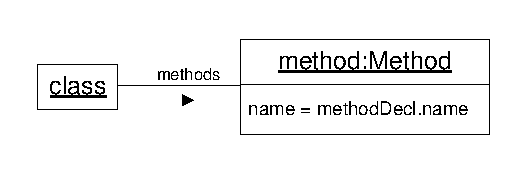
\includegraphics[scale=1]{figures/ObjectConstraint}
  \caption{Matching Pattern with an Attribute Constraint}
  \label{fig:objectConstraint}
\end{figure}

In the example, we match a method being contained in the class represented by the object variable \fe{theClass}. 
The match is restricted to a method which has the name "getName".

The values of attributes that are not restricted by an attribute constraint are not considered during the matching. 
Thus, they may have an arbitrary value. 
In the current version of story patterns, attribute constraints need to be specified using OCL~\cite{OCL}. 
Besides equality checks, all comparative operations on the attributes of an object supported by OCL can be used as object constraints. 

Besides attribute constraints, \emph{attribute assignments} can be used to change the value of an attribute during the application of a story pattern. 
Thus, attribute assignments are considered to be part of the RHS. 
When using attribute assignments, the value of the attribute is not considered while matching the LHS to the instance model. 
Figure \ref{fig:attributeAssignment} shows an example.

\begin{figure}[htbp]
  \centering
  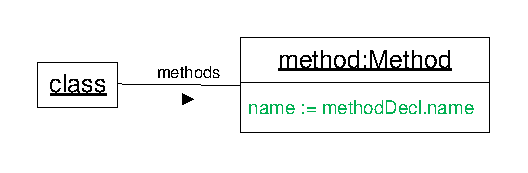
\includegraphics[scale=1]{figures/AttributeAssignment}
  \caption{Using an Attribute Assignment}
  \label{fig:attributeAssignment}
\end{figure}

In the example, the story pattern matches a method with an arbitrary name in the class \fe{theClass}. 
Then, the name of the method is changed to \emph{"getMethodName"}. 

The concrete syntax of an attribute assignment is
\begin{lstlisting}
 <attributeAssignment> ::= #Attribute.name ':=' Expression
\end{lstlisting}
The expression is to be specified using OCL. 
The type of the return value of the OCL expression must be assignable to the type of the attribute. 
Since the attribute value is changed as part of the RHS, the assignment is visualized in green color.

Story patterns also enable to use both, an attribute constraint and an attributed assignment for the same attribute inside one object variable. Then, the attribute constraint is used during the matching step. The attribute value of the object matched to the corresponding object variable is then changed as specified by the attribute assignment while enforcing the RHS.

\begin{figure}[htbp]
  \centering
  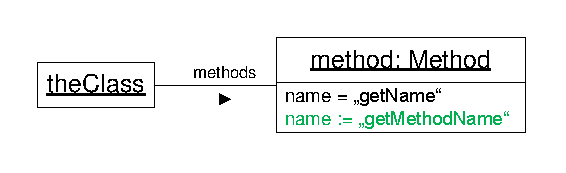
\includegraphics[scale=1]{figures/AttributeConstraintAndAssignment}
  \caption{Using an Attribute Constraint and an Attribute Assignment on the Same Attribute}
  \label{fig:attributeConstraintAndAssignment}
\end{figure}

Figure~\ref{fig:attributeConstraintAndAssignment} combines the story patterns of Figure~\ref{fig:objectConstraint} and~\ref{fig:attributeAssignment}. The story pattern matches an object of type \fe{Method} which has the name \fe{getName}. If the matching was successful, the name of the object bound to \fe{method} is set to \fe{getMethodName} as defined by the attribute assignment.

The OCL statements we allow for attribute constraints and attribute assignments must not traverse the references of the object variables.
Both may only use the attributes of object variables in the same story pattern and arbitrary arithmetic, comparing, and logical operations on them. 





%\ext  %--- Comment this line to include object sets into the document
{
\subsection{Collection Variables}
\label{sec:StoryPatterns:collectionvariables}

Collection variables are special cases of object variables.
They represent an arbitrary number of objects in an instance model that are of the same type.
Thus, a collection variable has the type of the objects within the collection\footnote{We do not
explicitly model collection objects in story diagrams. The type of a collection variable is that of the contained objects and not the type of a collection object like 
\texttt{java.util.Collection}}.

Figure~\ref{fig:CollectionVariableExample} depicts an example story pattern that
contains a collection variable \fe{methods}. During the matching, all
methods in the class that is bound to the object variable \fe{myClass} are
bound to the collection variable \fe{methods}.

\begin{figure}[htb]
  \centering
  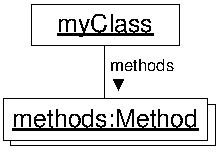
\includegraphics[scale=0.9]{figures/CollectionVariableExample}
  \caption{Collection Variable Example}
  \label{fig:CollectionVariableExample}
\end{figure}

The elements in collection variables are always ordered.
Collections can be specified to only contain unique elements or to allow the same element to be contained multiple times.
This leads to two different types of collections: ordered sets and lists.
Their semantics are similar to collection types in OCL: Elements in
ordered sets are ordered and unique. Elements in a list are ordered, but not necessarily
unique.

Figure~\ref{fig:CollectionVariableTypes} depicts the concrete syntax of the two collection types.

\begin{figure}[htb]
  \centering
  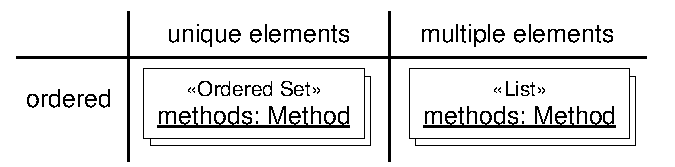
\includegraphics[scale=0.8]{figures/CollectionVariables}
  \caption{Types of collection variables: Ordered Set and List}
  \label{fig:CollectionVariableTypes}
\end{figure}


Two matched collection variables in the same story pattern do not have to be disjoint.
Thus, isomorphism is not enforced for the content of two or more collection variables.
Link variables between two collection variables are not allowed.

An attribute determines if the collection represented by a collection variable can be empty. 
If this is the case, a collection variables is considered to be optional in a
matching. Additionally, object constraints can be used to specify the allowed size of
the collection using OCL.

As the matching of collection variables is implicitly optional, their binding semantics cannot be set to ``optional'', explicitly.
Negative collection variables are not allowed.
Furthermore, collection variables in combination with a \create binding operator
are not allowed: collection variables can only be used in combination with the
binding operators ``check only'' or \destroy.

%\todomcp{explain set size expressions (do we change the name?)}
%\tododt{We should call the formerly known ObjectSetSizeExpression simply
%CollectionSizeExpression.}
%\todomvd{According to the meeting on May, 25th, set size expressions are
%omitted in v0.2. We can use OCL instead.}

%\todomcp{If we bind an object set, can we use the bound object in other story
%pattern? E.g., to insert all elements bound by the object set into a container
%via a containment link?}
%\tododt{Yes, but I would use another concrete syntax (see
%Figures~\ref{fig:reuseObjSet1}, \ref{fig:InclusionLinksExample1}).}

%\begin{figure}[htb]
%		\centering
%		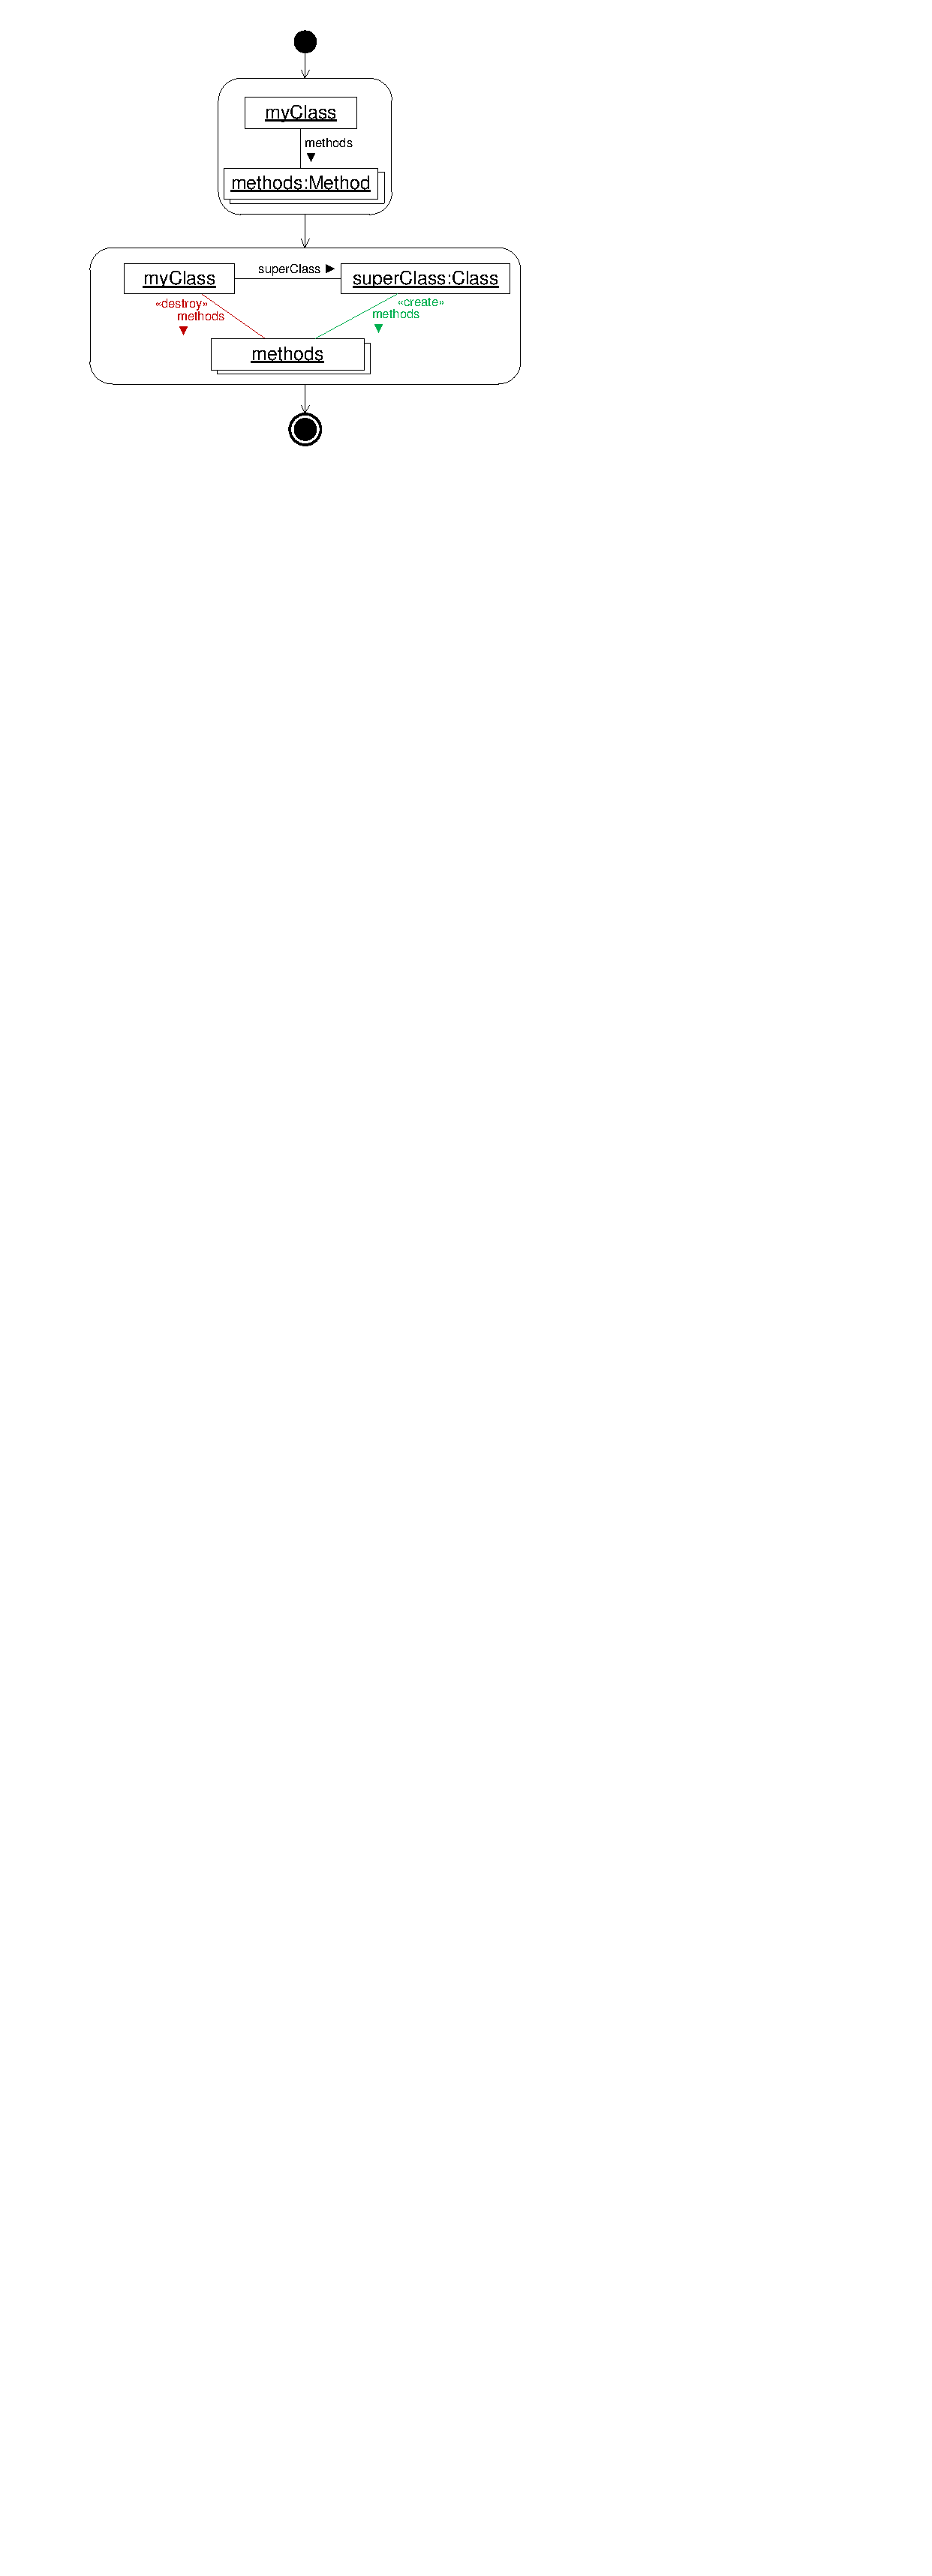
\includegraphics[scale=.8]{figures/ReuseObjectSet1}
%  	\caption{Reuse Objects in a Set}
%  	\label{fig:reuseObjSet1}
%\end{figure} 

%\todomcp{A collection variable contains no ObjectSetSizeExpression and no
%object is matched into the object set: collection variable is interpreted as
%optional and the matching succeeds.} 
%\tododt{We still should add an attribute to \fe{CollectionVariable} to
%distinguish the cases where at least one object should be matched or any number
%of objects including zero should be matched. Stephan also wanted this
%expressiveness.}


}%------ End of collection variable section


\subsection{Inclusion Links}
\label{sec:StoryPatterns:inclusion}

There are cases when you want to add additional objects to a set of objects matched to a collection variable
as described in Section~\ref{sec:StoryPatterns:collectionvariables}.
For example, when collecting all methods in a class hierarchy that comply to a certain method signature,
you would go through all classes in the hierarchy and add complying methods step by step.
Since a collection variable does not explicitly represent a collection object in
the sense of Java (as described in Section~\ref{sec:StoryPatterns:collectionvariables},
we need a way to describe the addition or removal ofobjects to or from such an object collection
as well as checking if an object is included in an object collection.
We introduce \emph{inclusion links} for this purpose.

\begin{figure}[htb]
	\begin{minipage}{.43\textwidth}
		\centering
		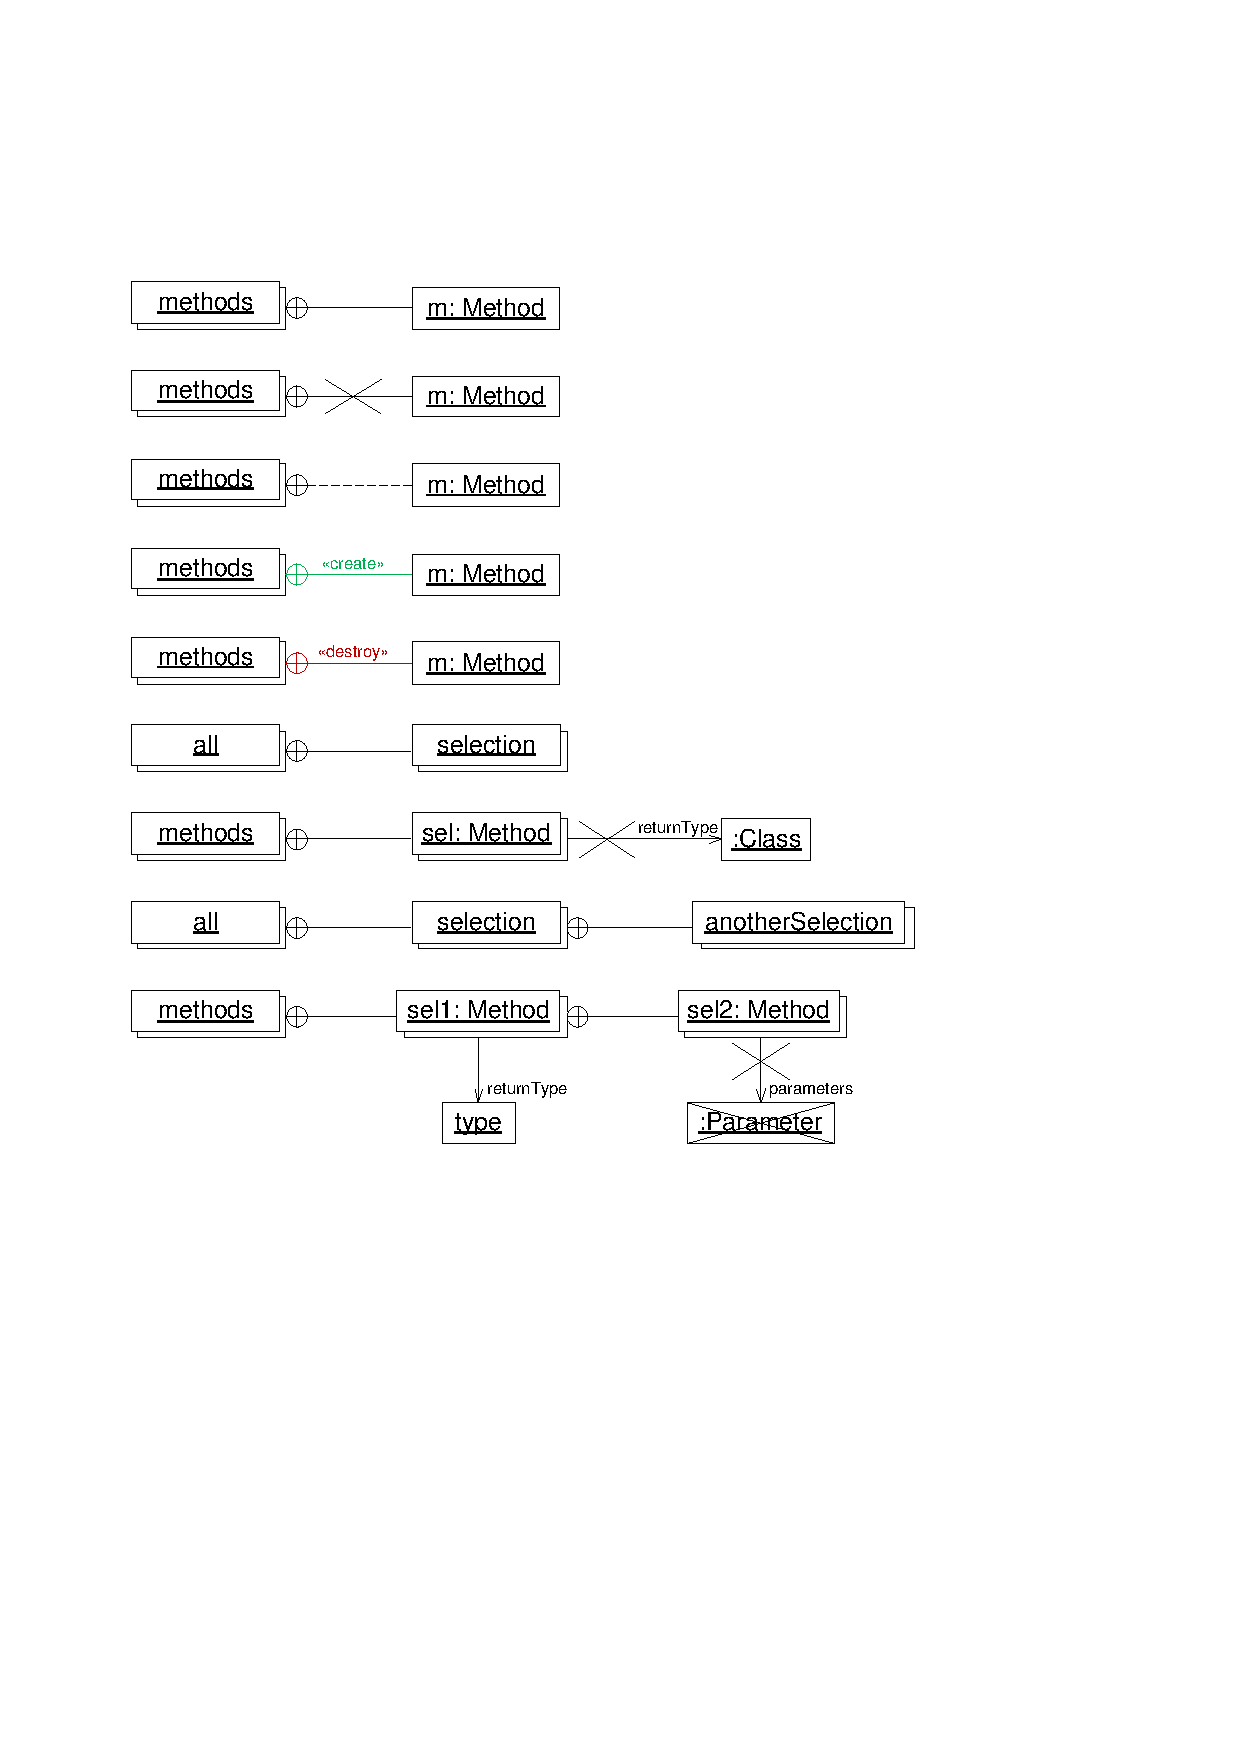
\includegraphics[width=\linewidth]{figures/InclusionLinks}
    \caption{Notation of Inclusion Links}
    \label{fig:InlucionLinks}
	\end{minipage}
  \hfill
  \begin{minipage}{.47\textwidth}
  	\centering
		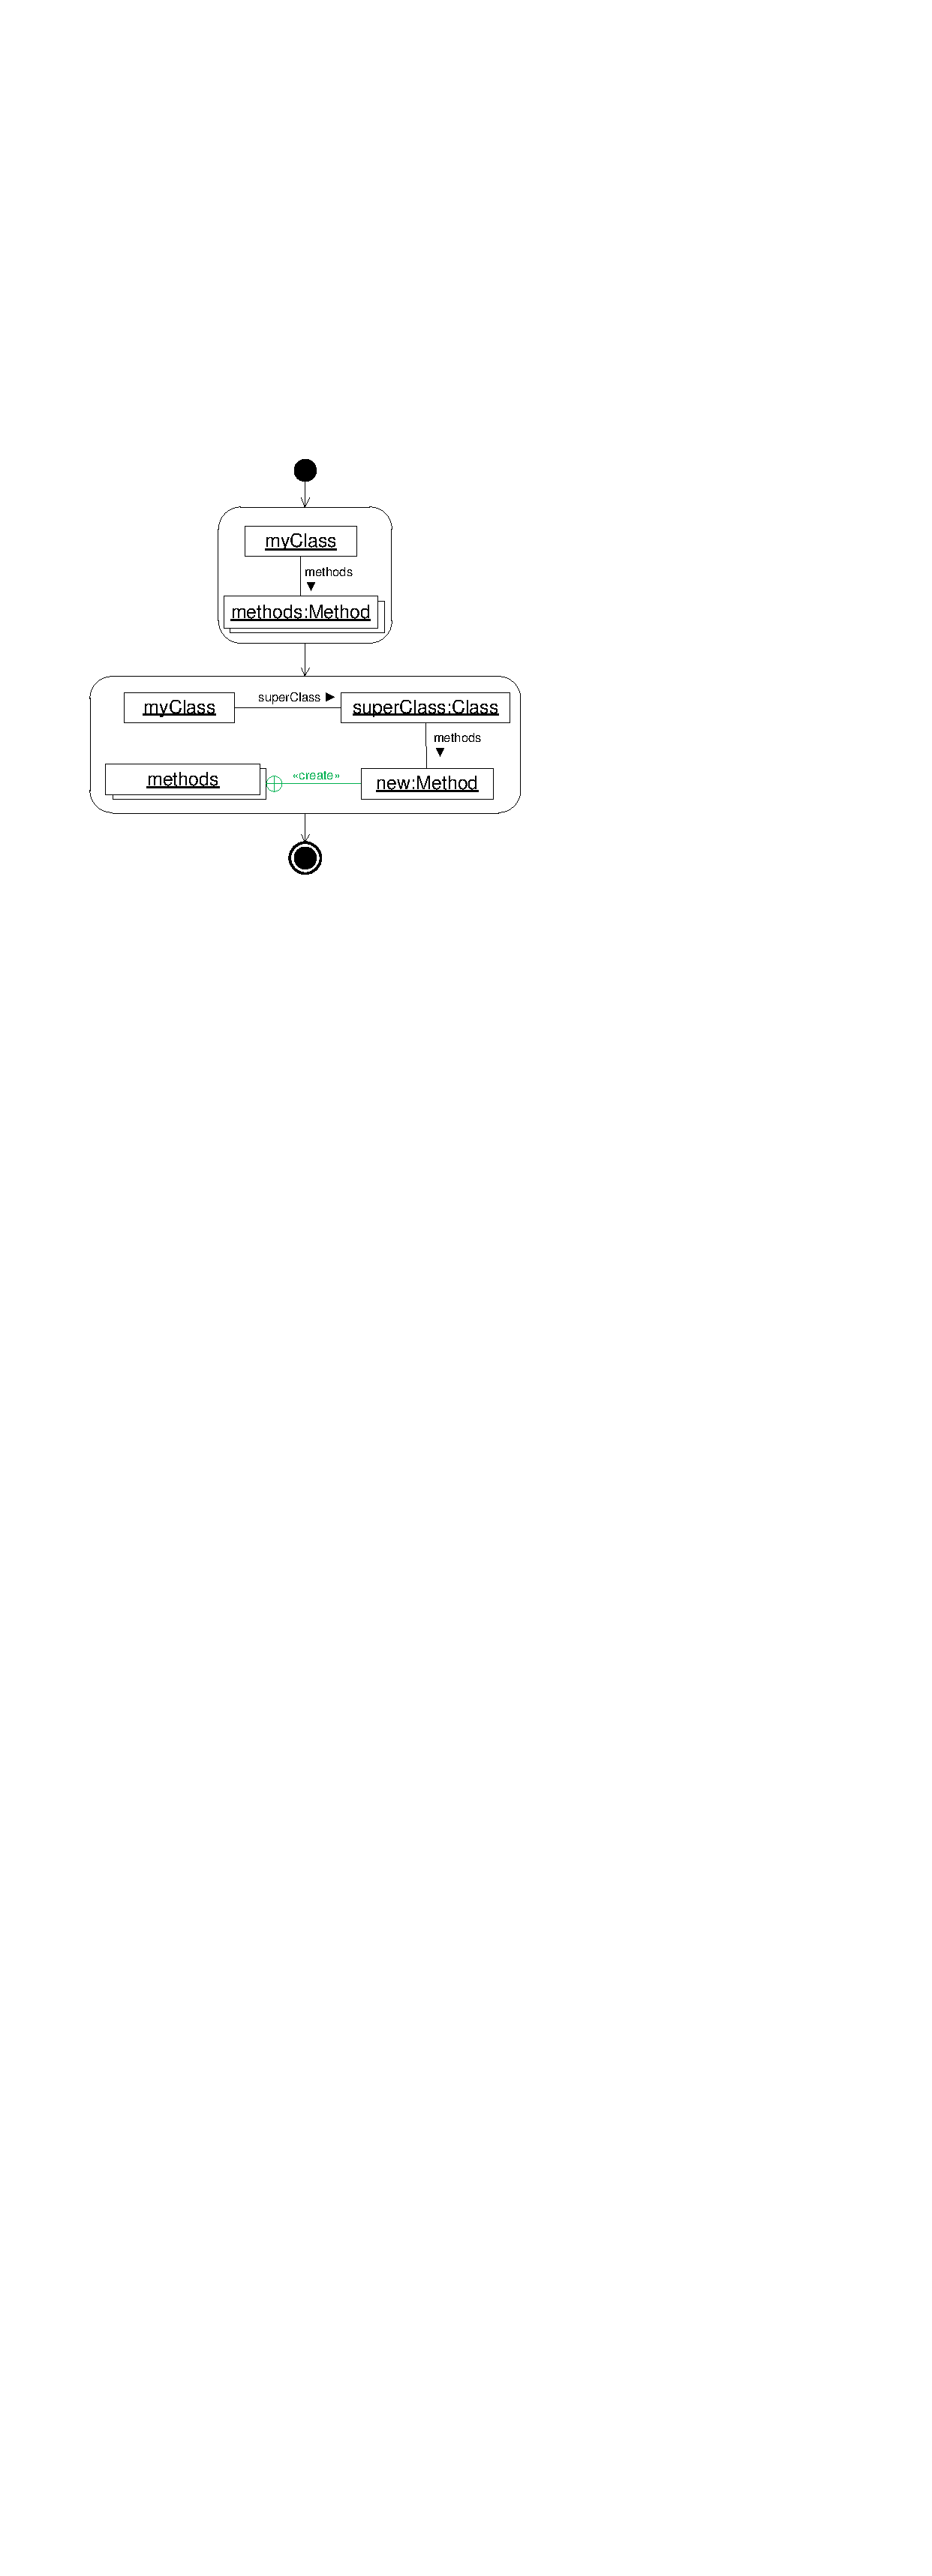
\includegraphics[width=\linewidth]{figures/InclusionLinksExample1}
    \caption{Add an Object to a Collection}
    \label{fig:InclusionLinksExample1}
	\end{minipage}
\end{figure}

An inclusion link represents a containment relation between two variables in a story pattern.
It can be used between a collection variable and another variable to specify that
an object (or a set of objects) represented by a variable is contained in an object set represented by a collection variable.
An inclusion link is represented by a line between a collection variable and another object
variable as illustrated in Figure~\ref{fig:InlucionLinks}~a).
The circle containing a plus determines which of the two sides of the link is containing the other one.
In Figure~\ref{fig:InlucionLinks}~a), the collection \fe{methods} contains an object \fe{aMethod}.

In contrast to link variables that are typed over an association,
\tododt{In fact, these are one or two references.}
inclusion links are not typed at all.
They only represent a containment of an object in a collection of objects.
But similar to link variables, this relation can be checked to be existent between a collection and an object
or be used to match new objects.
While the pattern in Figure~\ref{fig:InlucionLinks} a) specifies to check if the object \fe{aMethod} is contained in the collection \fe{methods},
the pattern in Figure~\ref{fig:InlucionLinks} b) specifies to match a \fe{Method} object which is contained in the collection \fe{methods}.

Similar to other links, inclusion links can be used with object variables that are bound, unbound, or maybe-bound.
Inclusion links can also be negative or optional and can be combined with \create\ or \destroy\ stereotypes (see Figure~\ref{fig:InlucionLinks} a) to f)).
Case c) in Figure~\ref{fig:InlucionLinks} defines that the matching is only successful if no \fe{Method} object can be found in the \fe{methods} collection.
Accordingly, case d) specifies to optionally match a \fe{Method} object contained in the \fe{methods} collection
(see the description of binding semantics in Section~\ref{sec:StoryPatterns:binding:semantics} for details).
Case e) specifies to create an inclusion relation between the object \fe{aMethod} and the collection \fe{methods},
i.e., to add the object \fe{aMethod} to the collection \fe{methods}.
Analogously, case f) specifies to remove the object \fe{aMethod} from the collection \fe{methods}.
Furthermore, inclusion links can also be used between two collection variables as illustrated in Figure~\ref{fig:InlucionLinks} f)
to check if all objects in the collection \fe{selection} are contained in the collection \fe{all}.

By means of inclusion links, a collection variable that has been matched to a set of objects
can be modified afterwards by adding or removing objects.
Using story diagrams as described in Section~\ref{sec:StoryDiagrams},
one can, for example, collect a set of \fe{Method} objects in a collection \fe{methods}
as illustrated in the first story node in Figure~\ref{fig:InclusionLinksExample1}
and then add another \fe{Method} object to the same collection in a following story node that reuses the previously matched set of objects.

\begin{figure}[htb]
  \centering
  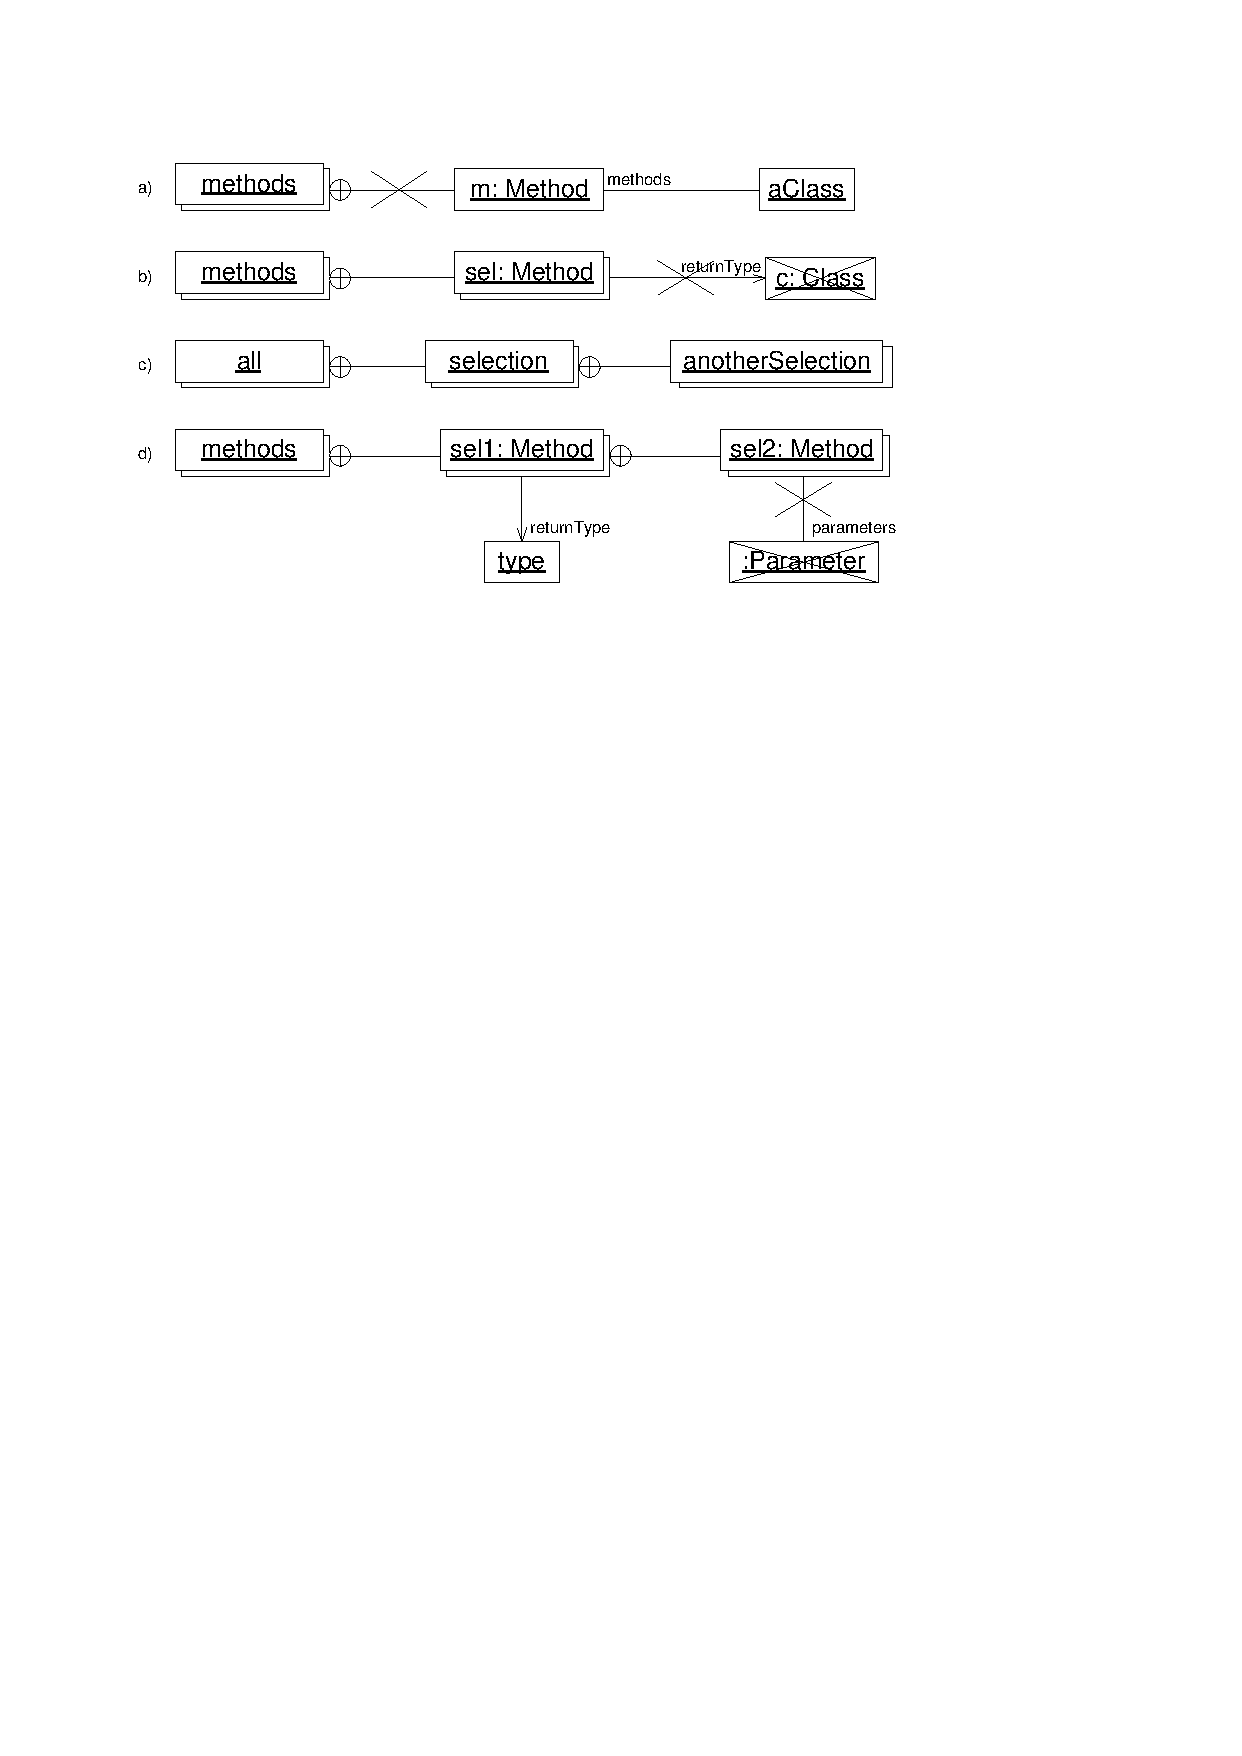
\includegraphics[scale=0.8]{figures/InclusionLinksExamples}
  \caption{Exemplary Uses of Inclusion Links}
  \label{fig:InlucionLinksExamples}
\end{figure}

Inclusion links can be used in combination with link variables.
In Figure~\ref{fig:InlucionLinksExamples} we give some examples for possible uses.
In case a) the story pattern specifies that a \fe{Method} object is to be found which is defined in a class \fe{aClass},
but which is not contained in the collection \fe{methods}.
Case b) specifies to find a collection \fe{sel} of \fe{Method} objects which are contained in the collection \fe{methods}
and do not have a return type that is a \fe{Class} object.
The pattern in case c) checks whether a set of objects described by the collection \fe{all} contains another set of objects described by the collection \fe{selection}
which in turn contains another set of objects described by the collection \fe{anotherSelection},
i.e., \fe{anotherSelection} is a subset of \fe{selection} and \fe{selection} is a subset of \fe{all}.
The pattern in case d) specifies to find two object sets that are subsets of another set.
First, a collection \fe{sel1} of \fe{Method} objects which have the return type \fe{type} is to be found in the collection \fe{methods}.
Second, a collection \fe{sel2} of \fe{Method} objects which additionaly have no parameters is to be found in the collection \fe{sel1}.


\subsubsection{Feasible Uses of Inclusion Links}
\label{sec:StoryPatterns:inclusion:feasible}

Inclusion links can be used exactly like link variables except that the source of an inclusion link has to be a collection variable.

Inclusion links can be used with all available binding semantics as described in Section~\ref{sec:StoryPatterns:binding:semantics}.
Consequently, if you replace a negative or optional link variable in Figures~\ref{fig:negativeObjects} and \ref{fig:optionalObjects}
with a negative or optional inclusion link
(independent of the inclusion link's direction and assuming that an inlucion link's source is a collection variable),
you get the feasible combinations of binding semantics used with inclusion links.

Moreover, you get all feasible combinations of binding operators and inclusion links from
Table~\ref{tab:bindingCombinations_links} in Section~\ref{sec:StoryPatterns:binding:operators}.

\begin{figure}[htbp]
  \centering
  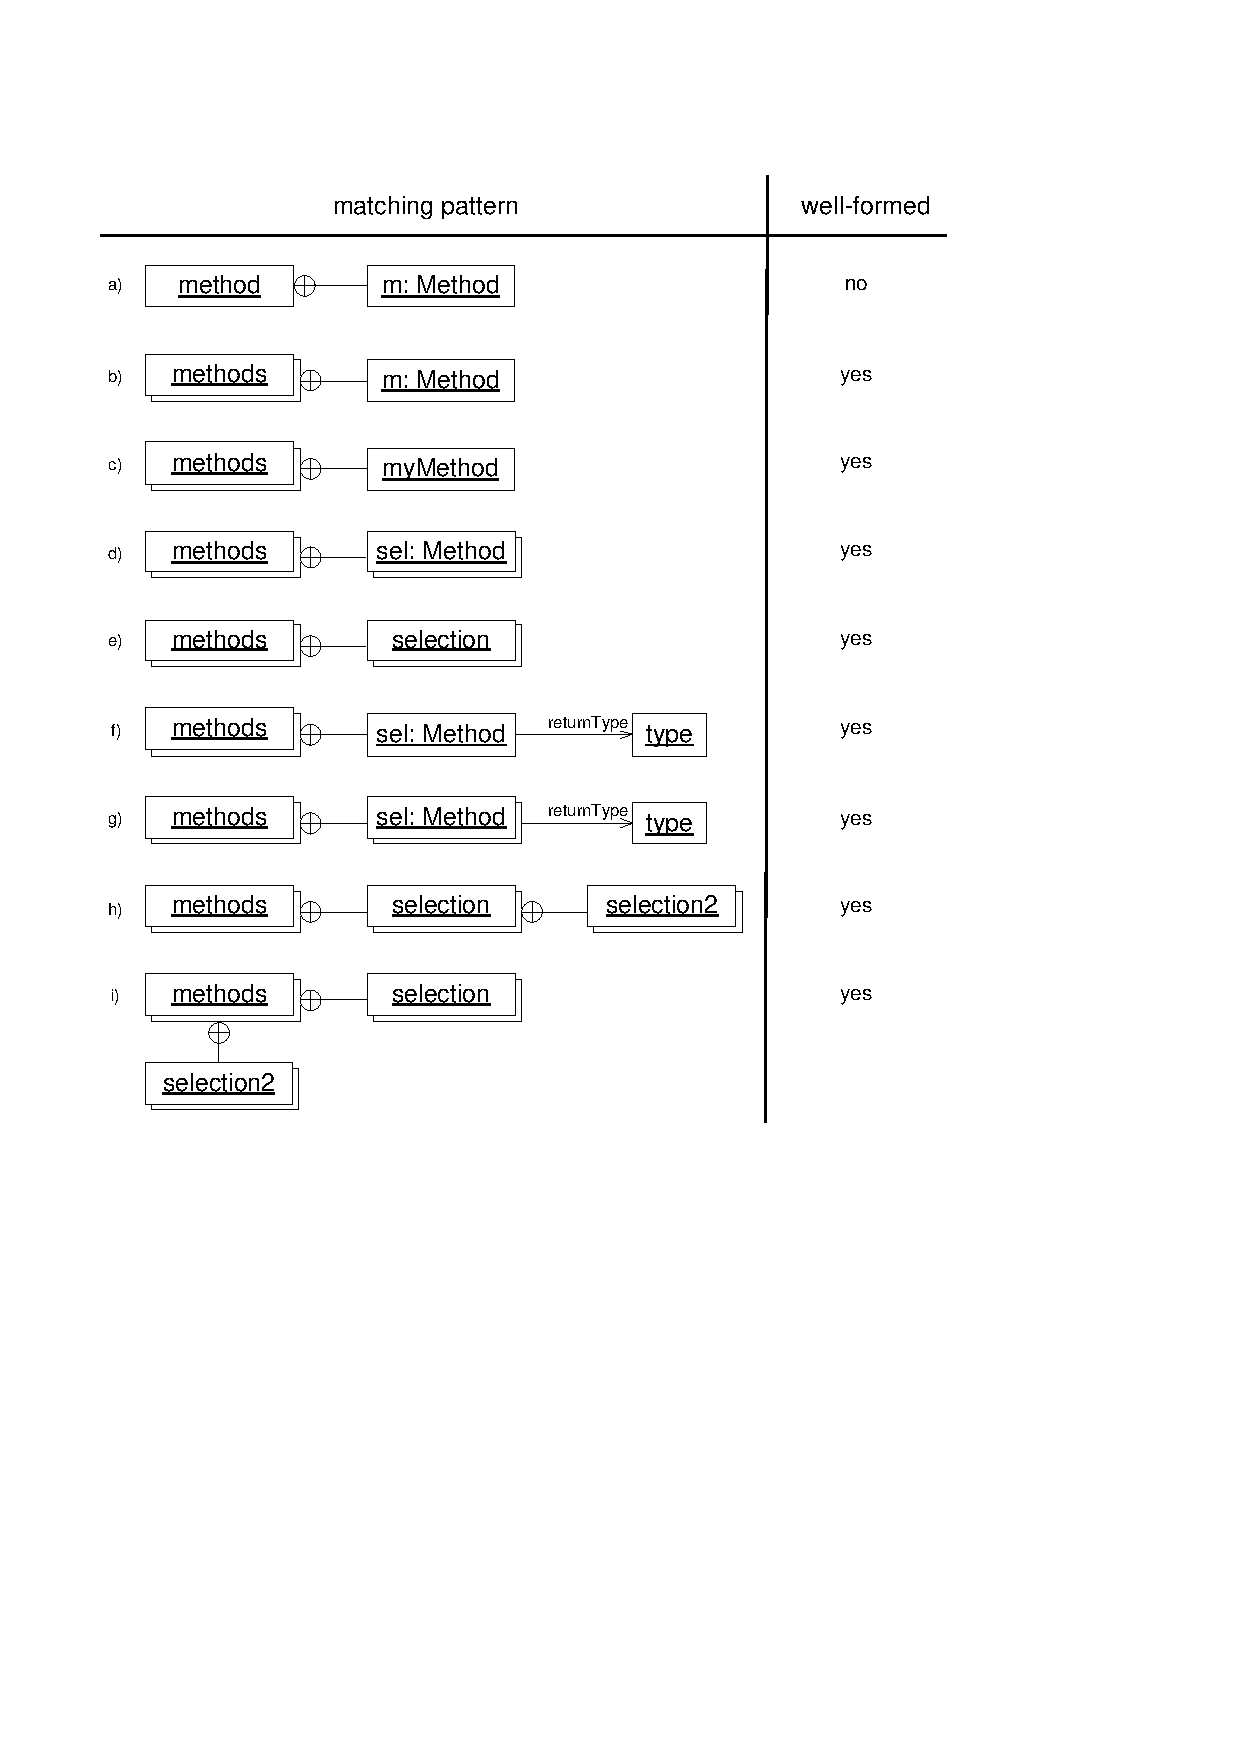
\includegraphics[scale=0.8]{figures/InclusionLinksWellFormedness}
  \caption{Well-formedness of inclusion links}
  \label{fig:InlucionLinkWellFormedness}
\end{figure}

In addition, different combinations of collection variables connected to a bound or unbound variable and
to a single object variable or a collection variable are feasible as illustrated in Figure~\ref{fig:InlucionLinkWellFormedness}.


\subsubsection{Collection Operations with Inclusion Links}
\label{sec:StoryPatterns:inclusion:BagsSetsEtc}

Inclusion links cannot only be used between a collection variable and a single object variable
as shown in Figure~\ref{fig:InlucionLinks} (p.~\pageref{fig:InlucionLinks}),
but also between two collection variables as shown in Figure~\ref{fig:InlucionLinkCollections}.
The semantics for this case are explained in the following.

\begin{figure}[htb]
  \centering
  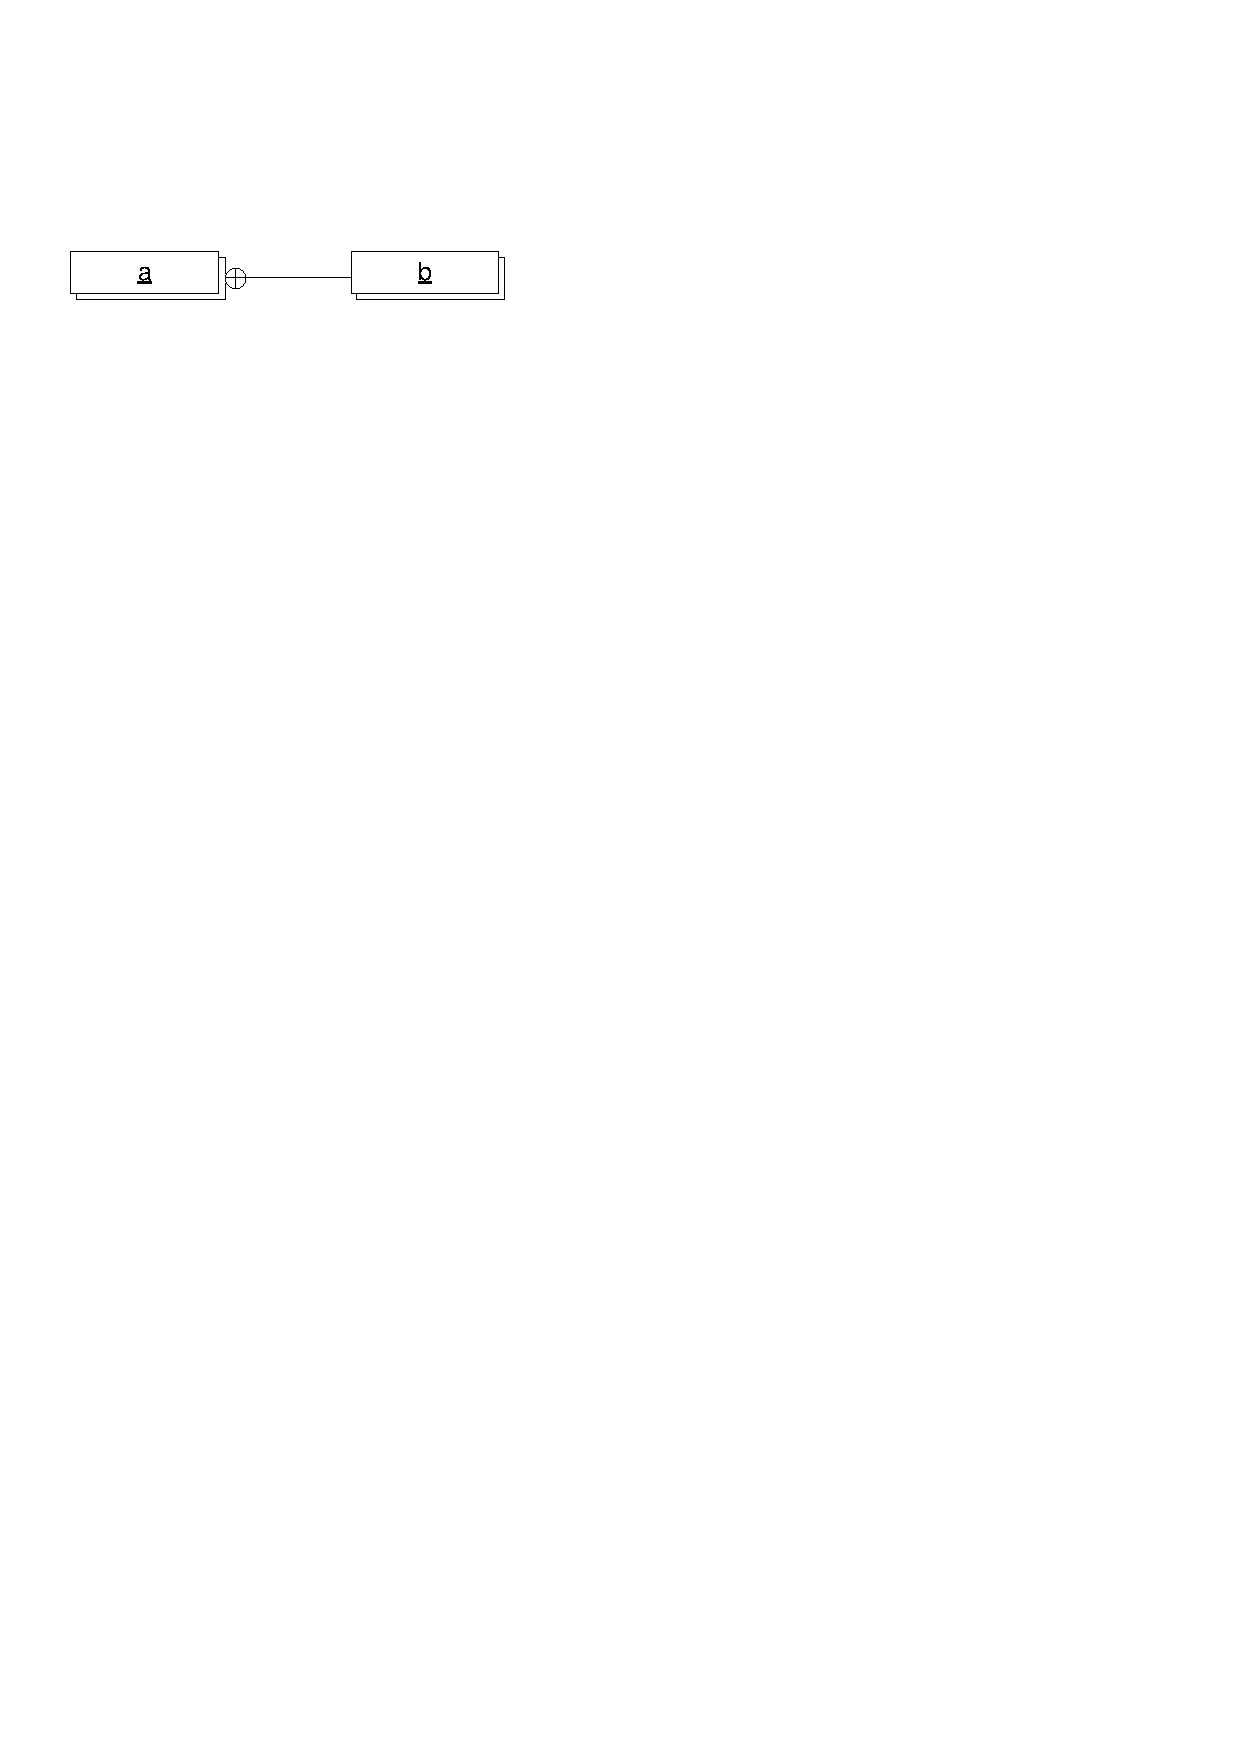
\includegraphics[scale=0.8]{figures/InclusionLinksSetsCheck}
  \caption{Inclusion Link Between Two Collections}
  \label{fig:InlucionLinkCollections}
\end{figure}

An inclusion link between two collection variables represents a containment relation between two sets of objects, i.e., between two collections.
In case of the illustration in Figure~\ref{fig:InlucionLinkCollections},
the collection \fe{b} depicts a subset of the set represented by the collection \fe{a} (mathematically $b \subseteq a$).
Interpreting the Figure~\ref{fig:InlucionLinkCollections} as a story pattern,
it describes to check if the elements in collection \fe{b} are also contained in the collection \fe{a}.

In Section~\ref{sec:StoryPatterns:collectionvariables} we introduced different types of collection variables.
We distinguish between ordered sets and lists.
Sets contain an element mostly once (\emph{unique} property) while lists can contain an element arbitrarily often.
Consequently, the inclusion links between different types of collection variables have different semantics,
which are described in Table~\ref{tab:set_operations_with_inclusion_links}.
The first two columns determine the type of the collections \fe{a} and \fe{b}.
The third column determines if the inclusion link is to be checked, created or removed.
The last column describes the semantics.

The main difference in the semantics of inclusion links stems from the unique or non-unique property of the collections.
If \fe{a} is a set and the binding operator is \fe{CHECK\_ONLY}, the execution of a story pattern
only checks if all objects in \fe{b} are contained (once) in \fe{a}
(mathematically $a \supseteq b$).
In contrast, if \fe{a} is a list (which can contain the same object arbitrarily often),
the story pattern execution ensures that the objects in \fe{b} are not only contained at least once in \fe{a},
but also at least as often as in \fe{b}.
If, for example, \fe{b} contains an element \fe{x} twice, then \fe{a} has to contain \fe{x} at least twice, too.
Otherwise, the matching of the story pattern fails.

An inclusion link with the binding operator \create\ describes to add all objects from \fe{b} to \fe{a}.
If \fe{a} is a set, the story pattern execution only adds each object from \fe{b} to \fe{a}
if \fe{a} does not already contain it. %(remember that sets contain each object mostly once).
Since story patterns only have ordered sets, the order of the objects in the collections have to be regarded.
The story pattern execution adds the objects from \fe{b} to the end of \fe{a} and keeps the same order as they had in \fe{b}.
If \fe{a} is a list, a similar adding operation is performed,
the objects from \fe{b} are added as often to \fe{a} as they are in \fe{b}.
This can be seen as a concatenation of two lists or as the union of two sets (mathematically $a \cup b$).

The binding operator \destroy\ used with an inclusion link and two collections as illustrated in Table~\ref{tab:set_operations_with_inclusion_links}
describes to remove all elements contained in \fe{b} from the collection \fe{a}.
If \fe{a} is a set, all occurrences of the objects in \fe{b} are removed from \fe{a} and the order of the remaining elements in \fe{a} is preserved.
If \fe{a} is a list and \fe{b} is a set, quite the same is done.
If an object contained in \fe{b} is contained more than once in \fe{a}, all of its occurrences in \fe{a} are removed.
This comes close to the mathematical relative complement operation (mathematically $a \setminus b$).
If both, \fe{a} and \fe{b} are lists,
only as many occurrences of the objects in \fe{b} are removed from \fe{a} as these are available in \fe{b}.
Furthermore, the removal starts at the beginning of the list \fe{a}.

\begin{table}[htbp]
%  \footnotesize
  \centering
%  \begin{longtable}{|l|l|c|p{4.6cm}|}
  \caption{Inclusion Links Between Two Collection Variables}
  \label{tab:set_operations_with_inclusion_links}
    \begin{tabular}{|l|l|c|p{4.6cm}|}
    \hline
    \textbf{Type of \fe{a}} & \textbf{Type of \fe{b}} & \textbf{Binding Operation} & \textbf{Semantics} \\
    \hline
    \multicolumn{3}{|c}{
      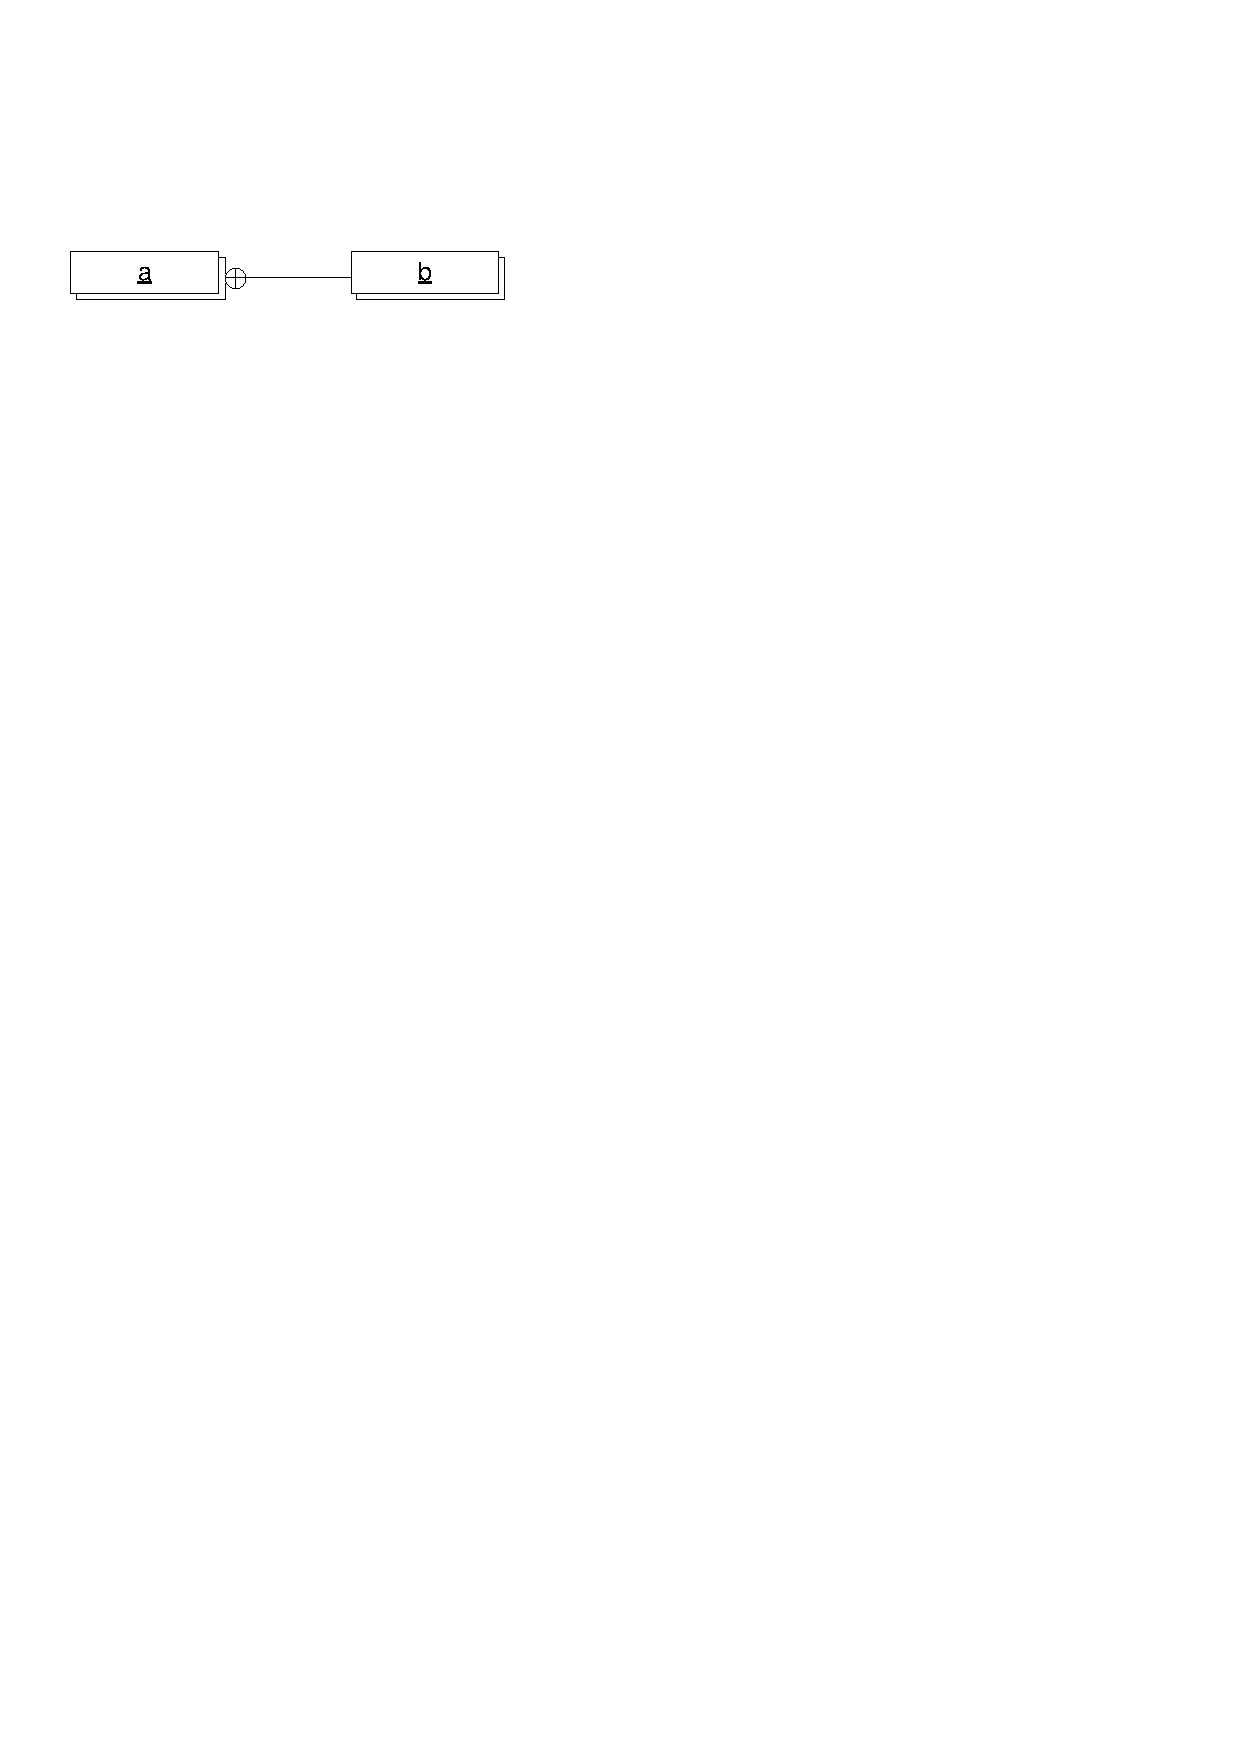
\includegraphics[scale=0.8]{figures/InclusionLinksSetsCheck}
    } & \\
    \hline
    Ordered Set & any & CHECK\_ONLY & Each element in \fe{b} is contained (once) in \fe{a}. \\[0.5em]
    List & any & CHECK\_ONLY & Each element in \fe{b} is contained at least as often in \fe{a} as in \fe{b}.\\
    \hline
    \multicolumn{3}{|c}{
      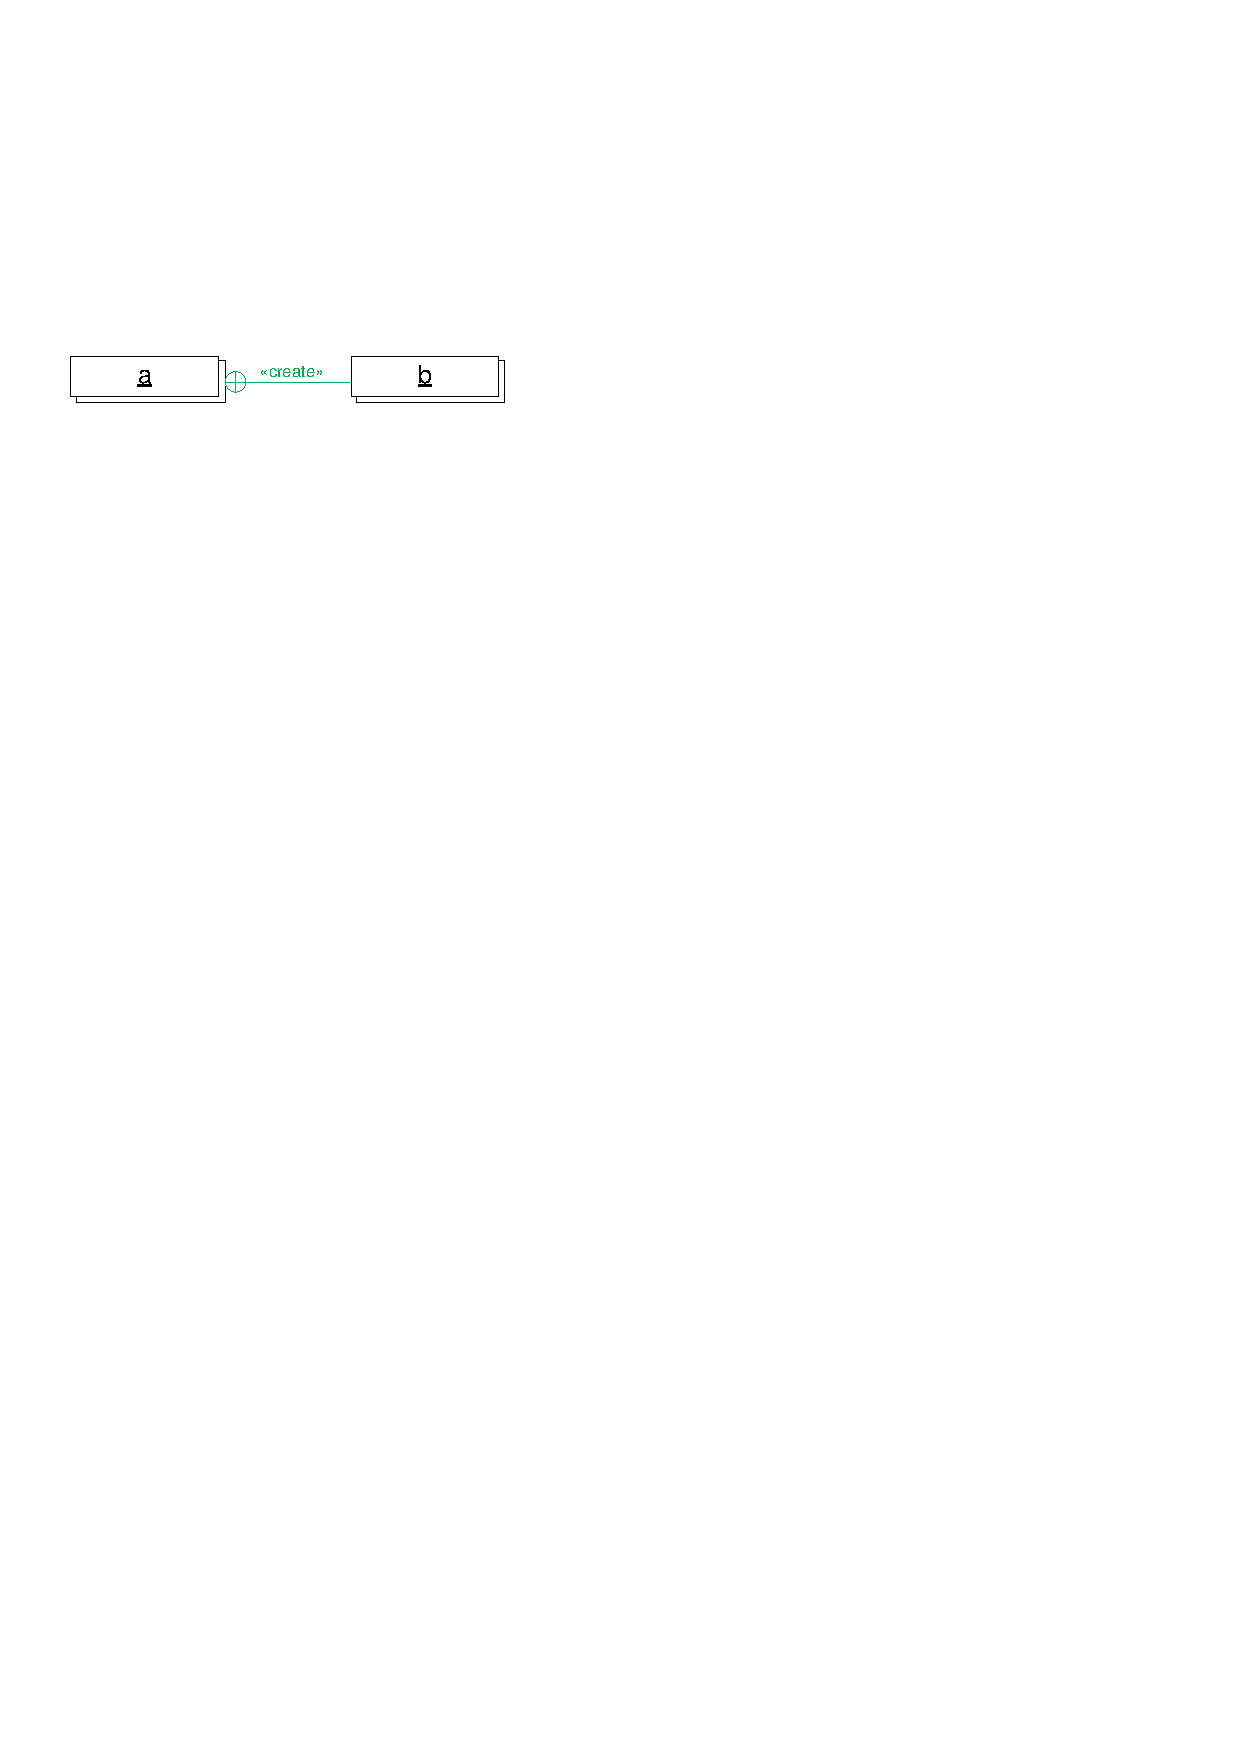
\includegraphics[scale=0.8]{figures/InclusionLinksSetsCreate}
    } & \\
    \hline
    Ordered Set & any & CREATE & Add all elements from \fe{b} to \fe{a} that are missing in \fe{a} to the end of \fe{a}, preserving the order of elements in \fe{b}.\\[0.5em]
    List & any & CREATE & Add all elements from \fe{b} to the end of \fe{a}, preserving the order of elements in \fe{b}.\\
    \hline
    \multicolumn{3}{|c}{
      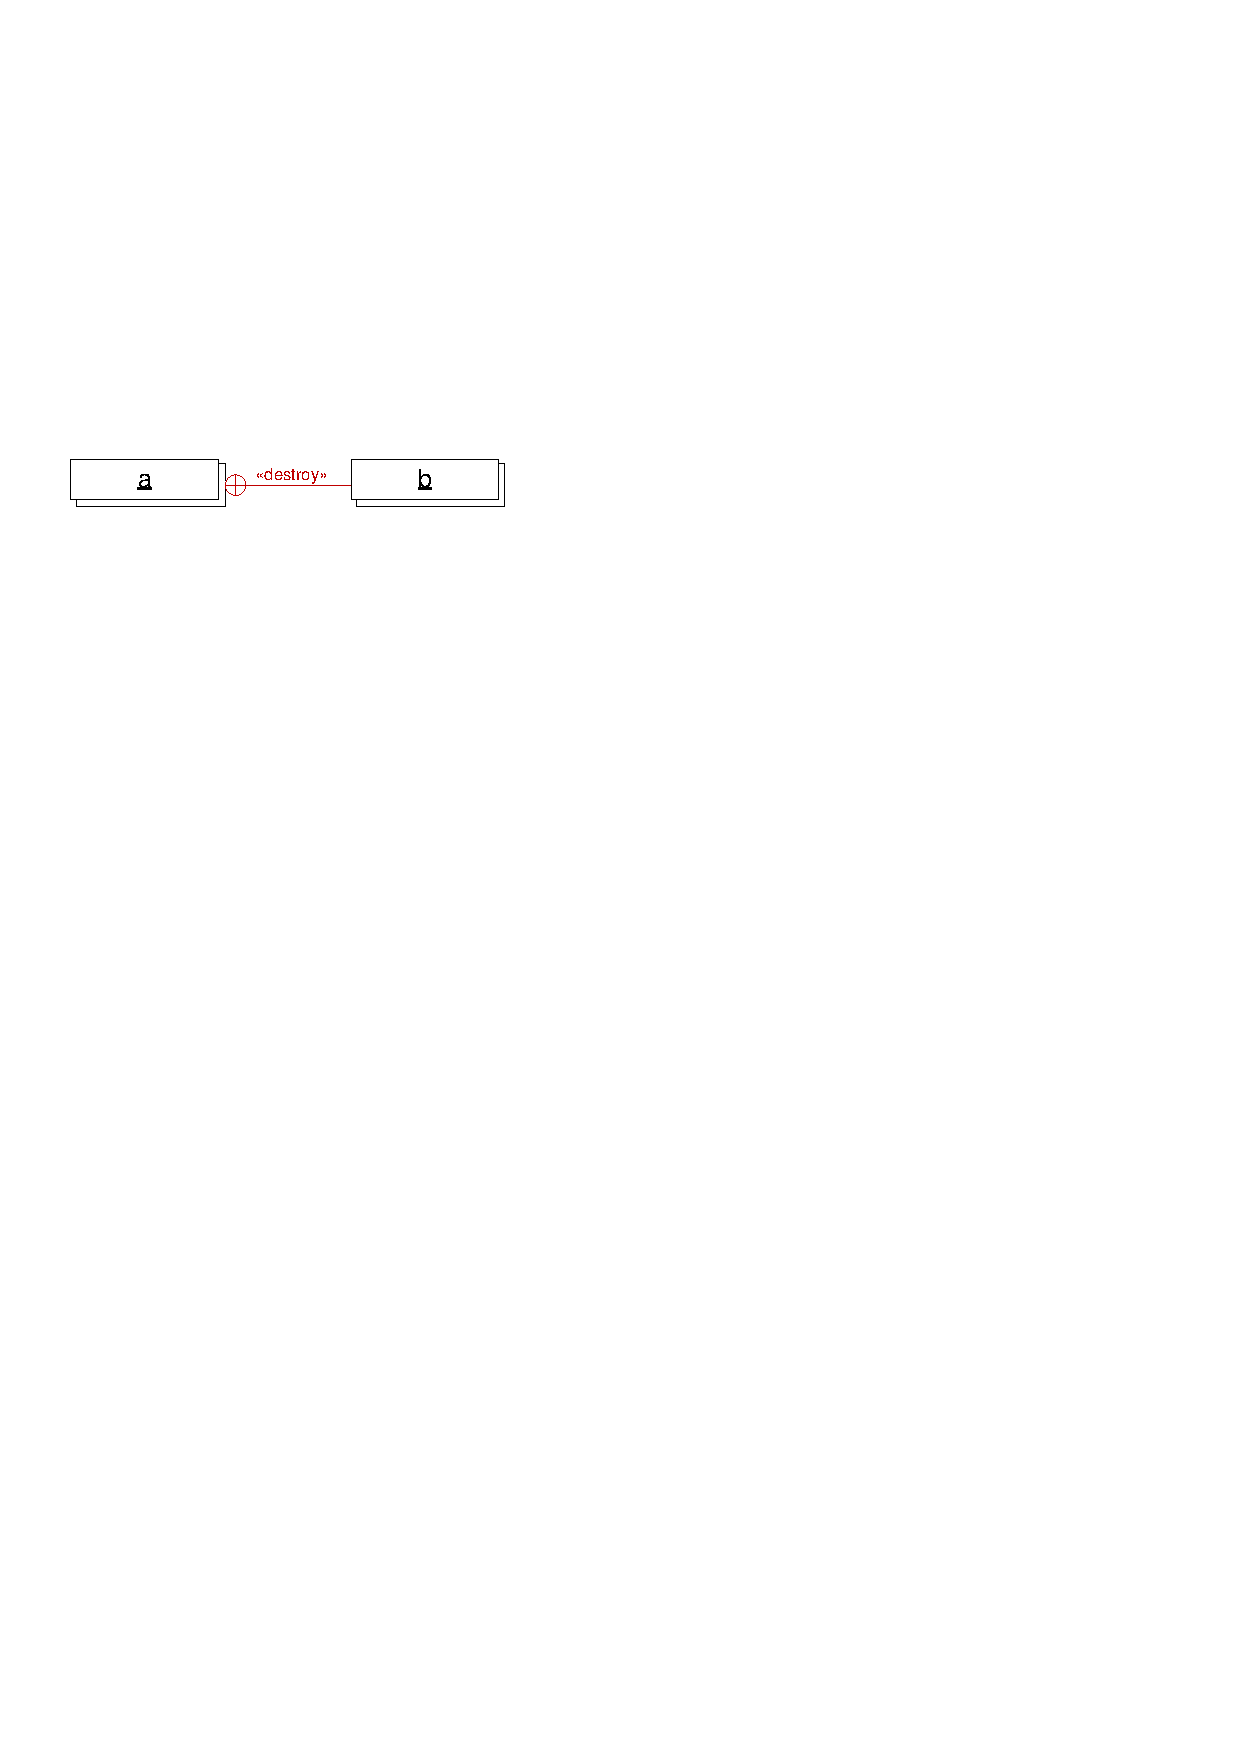
\includegraphics[scale=0.8]{figures/InclusionLinksSetsDestroy}
    } & \\
    \hline
    Ordered Set & any & DESTROY & Remove all elements in \fe{b} from \fe{a}, preserve the order of remaining elements in \fe{a}.\\[0.5em]
    List & Ordered Set & DESTROY & Remove \emph{all} occurrences of elements contained in \fe{b} from \fe{a}, preserve the order of remaining elements in \fe{a}.\\[0.5em]
    List & List & DESTROY & Starting at the beginning of the list \fe{a}, for each element in \fe{b} remove as many occurrences of the element in \fe{a} as it is available in \fe{b}, preserve the order of remaining elements in \fe{a}.\\
    \hline
    \end{tabular}
%  \end{longtable}
\end{table}


%\ext %--- Comment this line to include link constraints into the
{
\subsection{Link Constraints}
\label{sec:StoryPatterns:linkConstraints}

\tododt{The link constraints section is existing twice.}

Link constraints specify constraints on the absolute position of an element in an ordered reference (\emph{link position constraints}, Section~\ref{sec:StoryPatterns:linkConstraints:posConstraint}) or on the position of an element relative to another element (\emph{link order constraints}, Section~\ref{sec:StoryPatterns:linkConstraints:orderConstraint}). These constraints are only applicable to link variables that are typed by ordered multi-valued references. All other kinds of links cannot be adorned with link constraints.

%\begin{itemize}
%  \item FIRST = matches the first element in the list, requires one link variable
%  \item LAST = matches the last element in the list, requires one link variable
%%  \item INDEX = matches the element at the specified index, requires one link variable
%%  \todoch{Our lowest index value is 0, not 1.}
%  \item DIRECT\_SUCCESSOR = requires two link variables, target of the second one must be located directly after the target of the first one in the list
%  \item SUCCESSOR = requires two link variables, target of the second one must be located somewhere after the target of the first one in the list
%\end{itemize}


\subsubsection{Link Position Constraints}
\label{sec:StoryPatterns:linkConstraints:posConstraint}

A link position constraint applies to a link variable that is typed by a multi-valued ordered reference. It specifies that the target object of the constrained link has to be the \emph{first} or the \emph{last} element in that reference. Other link position constraints are not supported. 

The \emph{index} link constraint, which was available in earlier versions of story diagrams~\cite{WW01_ag}, is no longer supported. 
It was used to match an element which is located at a specific position in a multi-valued reference. 
However, that causes that upon creation of multiple elements it is not precisely defined where they are inserted into the list. 
In addition, the index may cause \emph{OutOfBounds} exceptions if the modeler specifies an invalid index.

Figure~\ref{fig:linkPositionConstraintFirst} shows an example of a link position constraint for matching the first element in a reference. The story pattern matches a \fe{FormalParameter} of the object which is bound to the object variable \fe{method}. The link position constraint \fe{\{first\}} specifies that the first \fe{FormalParameter} needs to be matched.

\begin{figure}[htbp]
\center
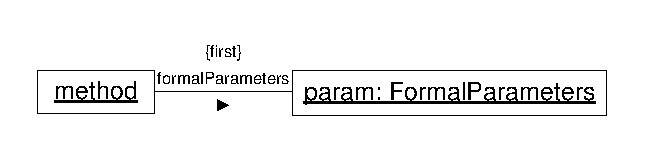
\includegraphics[width=0.75\columnwidth]{figures/LinkPositionConstraintFirst}
\caption{A \fe{\{first\}} link position constraint}
\label{fig:linkPositionConstraintFirst}
\end{figure}

Figure~\ref{fig:linkPositionConstraintLast} shows a similar story pattern, which matches the last \fe{FormalParameter} instead of the first one. This is specified by the link position constraint \fe{\{last\}}.

\begin{figure}[htbp]
\center
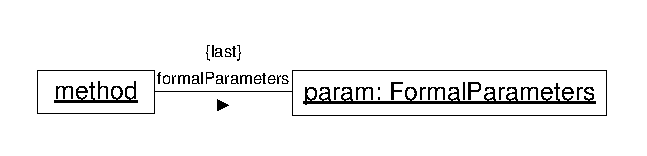
\includegraphics[width=0.75\columnwidth]{figures/LinkPositionConstraintLast}
\caption{A \fe{\{last\}} link position constraint}
\label{fig:linkPositionConstraintLast}
\end{figure}

If multiple link variables originate from the same object variable that refer to the same reference, only one of them may have a \fe{\{first\}} (or \fe{\{last\}}) link position constraint.

Link position constraints can be used with all feasible combinations of binding operators and binding semantics according to Table~\ref{tab:bindingCombinations_links}. For now, we discussed the semantics for using link position constraints for link variables with MANDATORY binding semantics and CHECK\_ONLY binding operator. If we use binding operator \create, the object is inserted at the specified position.
If the target element already exists in the reference but at a different position, the semantics of the create depends on the kind of the reference. 
If the reference requires objects to be unique in the reference, the target element is moved to the position specified by the create link variable. 
Otherwise, the element is added a second time at the specified position.
If we use binding operator \destroy, the object is bound as described before and then deleted.

Figure~\ref{fig:linkPositionConstraintCreate} shows an example for using a link position constraint at a link variable with binding operator \create. The link position constraint causes the created \fe{FormalParameter} to be inserted at the last position of the \fe{formalParameters} of \fe{method}.

\begin{figure}[htbp]
\center
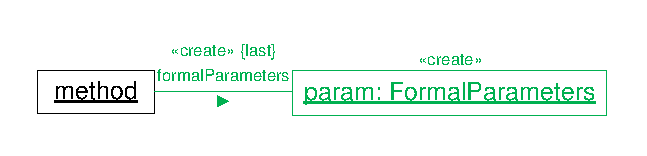
\includegraphics[width=0.75\columnwidth]{figures/LinkPositionConstraintCreate}
\caption{Link Position constraint at a created link.}
\label{fig:linkPositionConstraintCreate}
\end{figure}

If an OPTIONAL binding semantics is used, the matching will also be successful if no object at the specified position can be matched. Since we only restrict the position to the first or last position, this case will only apply if the link contains no objects at all. If the link variable additionally has binding operator \destroy, the object bound to the target object variable will be deleted. If the link variable additionally has binding operator \create, we have an optionally created link. If the object does not yet exist at the specified position, it is inserted following the rules for created links as described before. 

A combination with NEGATIVE binding semantics is also possible. If a link variable is negative and has a \fe{\{first\}} (or \fe{\{last\}}) link position constraint, then the object bound to the target object variable must not be the first (or last) object in the corresponding reference. That means, we negate the link position constraint rather than the whole link variable which causes a slight change of the NEGATIVE binding semantics of link variables.

%\todoch{How is the semantics of link position constraints on negative links as shown in Figure~\ref{fig:linkPositionConstraintNegative}? Two alternatives: 1) The target object is not the first (or last) element in the reference. That means we negate the link position constraint and not the whole link variable. 2) There exists no link pointing to the first (or last) element. That means we negate the whole link which in turn means that there is no element in the reference and the link position constraint has no effect. I prefer 1) even though it slightly changes the semantics of the negative binding semantics (because it is applied to the link constraint rather than the link itself).}

Figure~\ref{fig:linkPositionConstraintNegative} shows an example for a negative link with a link position constraint. The \fe{FormalParameter} which is bound to \fe{param} must not be the first \fe{formalParameter} of the method which is bound to \fe{method}.


\begin{figure}[htbp]
\center
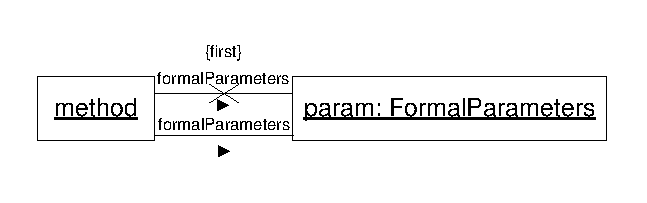
\includegraphics[width=0.75\columnwidth]{figures/LinkPositionConstraintNegated}
\caption{A negative link with a \fe{\{first\}} link position constraint}
\label{fig:linkPositionConstraintNegative}
\end{figure}



\subsubsection{Link Order Constraints}
\label{sec:StoryPatterns:linkConstraints:orderConstraint}

Link order constraints specify a relative order between two objects in a multi-valued ordered reference. A link order constraint therefore connects two link variables which we denote as the source link variable and target link variable of the link order constraint. Then, the object matched via the target link variable must either be the \emph{direct successor} or an  \emph{arbitrary successor} of the object matched via the source link variable.

Figure~\ref{fig:linkOrderConstraintDirectSuccessor} shows an example of a link order constraint requiring to match two subsequent \fe{FormalParameters} of \fe{method}. Therefore, the two link variables from \fe{method} to \fe{param1} and \fe{param2} are connected by a link order constraint \fe{\{next\}}. Then, the object matched to \fe{param2} must be a direct successor of the object matched to \fe{param1}.

\begin{figure}[htbp]
\center
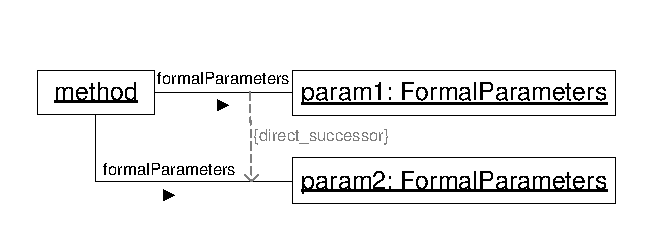
\includegraphics[width=0.75\columnwidth]{figures/LinkOrderConstraintDirectSuccessor}
\caption{A link order constraint specifying a \fe{\{direct\_successor\}}.}
\label{fig:linkOrderConstraintDirectSuccessor}
\end{figure}

Figure~\ref{fig:linkOrderConstraintSuccessor} shows an example of a link order constraint requiring to match two \fe{FormalParameters} of \fe{method} where one succeeds the other. Therefore, the two link variables from \fe{method} to \fe{param1} and \fe{param2} are connected by a link order constraint \fe{\{successor\}}. Then, the object matched to \fe{param2} must be an arbitrary successor of the object matched to \fe{param1}. The matching of the successor is non-deterministic. Thus, a matching retrieved for the story pattern in Figure~\ref{fig:linkOrderConstraintDirectSuccessor} is a valid matching for the story pattern in Figure~\ref{fig:linkOrderConstraintSuccessor} as well. A matching retrieved for the story pattern in Figure~\ref{fig:linkOrderConstraintSuccessor}, however, will not be a valid matching for the story pattern in Figure~\ref{fig:linkOrderConstraintDirectSuccessor} in the general case.

\begin{figure}[htbp]
\center
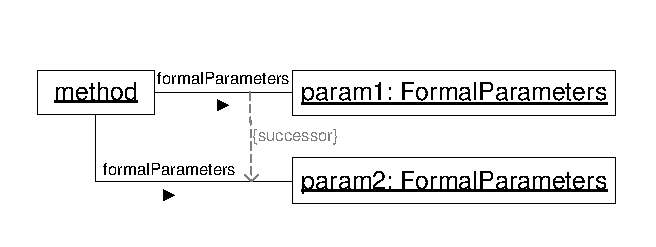
\includegraphics[width=0.75\columnwidth]{figures/LinkOrderConstraintSuccessor}
\caption{A link order constraint specifying a \fe{\{successor\}}.}
\label{fig:linkOrderConstraintSuccessor}
\end{figure}

Link order constraints can be applied to links that have a binding operator \create or \destroy. In case of \destroy, the matching is carried out as described before. In case of \create, links corresponding to the link variables are created in the instance model. The target objects are then inserted into the reference at the specified positions. If the source link variable (or target link variable) of the link order constraint has a \create binding operator, then the object is inserted directly before (or after) the object bound via the target (or source) link variable. We also apply this semantics if the link order constraint requires the objects only to be indirect successors to avoid non-determinism.

\begin{figure}[htbp]
\center
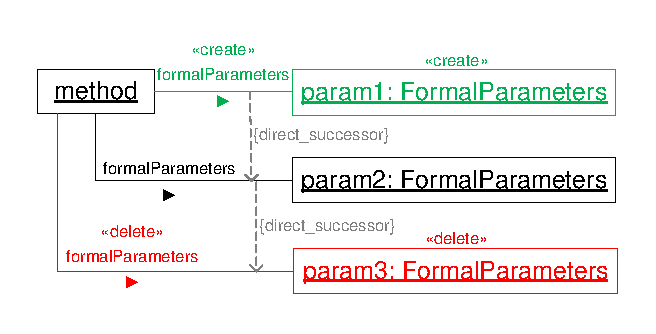
\includegraphics[width=0.75\columnwidth]{figures/LinkOrderConstraintDirectSuccessorCreateDelete}
\caption{Using link order constraints with binding operators \create and \destroy.}
\label{fig:linkOrderConstraintDirectSuccessorCreateDelete}
\end{figure}

Figure~\ref{fig:linkOrderConstraintDirectSuccessorCreateDelete} shows an example for using link order constraints with the binding operators \create and \destroy. The story pattern matches two successive \fe{FormalParameters} of \fe{method} and binds them to the object variables \fe{param2} and \fe{param3}. If the matching was successful, the parameter bound to \fe{param3} is deleted and removed from the reference. Then, a new \fe{FormalParameter} is created and inserted directly before \fe{param2}.

If a link variable with binding operator \create is the target link variable (or source link variable) of several \emph{indirect successor} link order constraints, then the target object of the link variable is inserted directly behind (or before) the object with the highest index. If  multiple link constraints are applied to the same link variable with binding operator \create, enforcing the right-hand side of the story pattern may fail if the link constraints are unsatisfiable for the reference.

If the reference already contains the target object of a create link variable, but at a position which does not satisfy the link order constraint, then there are two possibilities.  If the reference requires objects to be unique in the reference, the target element is moved to a position specified by the link order constraints. Otherwise, the element is added a second time at a position specified by the link order constraints. 

If both, the source link variable and the target link variable of the link order constraint, carry a binding operator, both need to carry the same binding operator. If one link variable has a binding operator \create and the other one has \destroy, then the reference for inserting the new object has been deleted before the object can be inserted. Since the semantics in undefined in that case, we forbid this case.

Link order constraints can be used in combination with an optional binding semantics of the source or target link variable. In case the link variable carries no binding operator or binding operator \destroy, the matching process is performed as described before. If no matching for the optional link variables satisfying the link order constraints can be found, the matching does not fail. If the a link variable carries an optional create, a matching which satisfies the link order constraints is searched. If no matching can be obtained, the rules for inserting an object into a reference as described above for non-optional link variables are applied.

Link order constraints may also be used in combination with a negative binding semantics of the source or target link variable. If a negative link variable is the target link variable of a \emph{direct successor} (or \emph{indirect successor}) link order constraint, then the target object must not be located directly after (of indirectly after) the object bound to the source link variable. If a negative link variable is the source link variable of a \emph{direct successor} (or \emph{indirect successor}) link order constraint, then the target object must not be located directly before (of indirectly before) the object bound to the target link variable. That means, we negate the link order constraint rather than the whole link variable if the link variable is the source or target link variable of a link order constraint. That causes a slight change in the definition of the negative binding semantics for link variables.

\begin{figure}[htbp]
\center
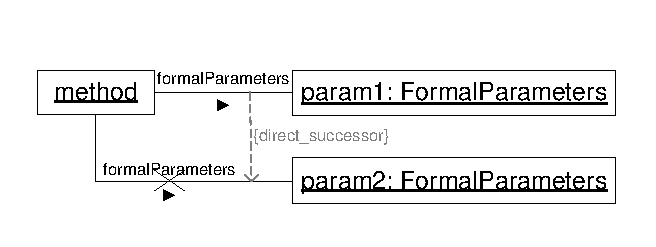
\includegraphics[width=0.75\columnwidth]{figures/LinkOrderConstraintDirectSuccessorNegative}
\caption{A link order constraint with a negative link.}
\label{fig:linkOrderConstraintDirectSuccessorNegative}
\end{figure}

Figure~\ref{fig:linkOrderConstraintDirectSuccessorNegative} shows an example of a negative link variable which is the target link variable of a \emph{direct successor} link order constraint. In the example, two \fe{FormalParameters} of \fe{method} are to be matched. The object bound to \fe{param1} may be an arbitrary \fe{FormalParameter}. The object variable \fe{param2} may be matched to any \fe{FormalParameter} of \fe{method} except for the \fe{FormalParameter} that is directly located behind the object bound to \fe{param1}.

It is possible to use multiple link order constraints on a negative link. Then, all of the specified conditions need to hold. However, for each link order constraint either the source link variable or the target link variable may be negative, but not both.

\begin{figure}[htbp]
\center
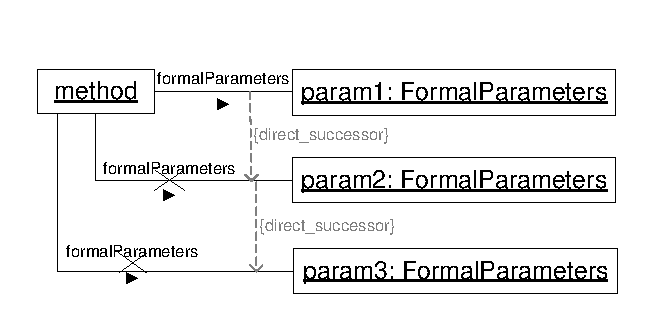
\includegraphics[width=0.75\columnwidth]{figures/LinkOrderConstraintDirectSuccessorNegative2}
\caption{Applying Multiple Link Order Constraints on a Negative Link Variable}
\label{fig:linkOrderConstraintDirectSuccessorNegative2}
\end{figure}

Figure~\ref{fig:linkOrderConstraintDirectSuccessorNegative2} shows an example of applying multiple link order constraint to a negative link variable. The story pattern matches three \fe{FormalParameters} of \fe{method}. The matching must fulfill the following conditions which are implied by the negative link variable from \fe{method} to \fe{param2} and the two link order constraints: \fe{param2} must not be an indirect successor of \fe{param1} and \fe{param3} must not be the direct successor of \fe{param2}. If only one of the two conditions is not fulfilled, then the story pattern does not match.

\begin{figure}[htbp]
\center
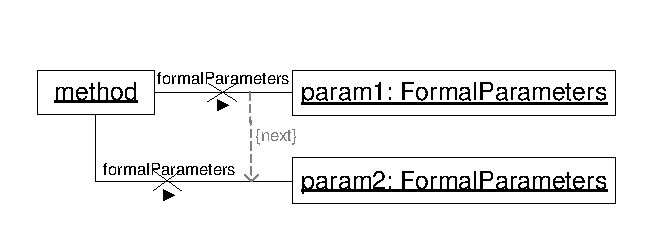
\includegraphics[width=0.75\columnwidth]{figures/LinkOrderConstraintDirectSuccessorNegative3}
\caption{Invalid Combination of Link Order Constraints and Negative Link Variables.}
\label{fig:linkOrderConstraintDirectSuccessorNegative3}
\end{figure}

Figure~\ref{fig:linkOrderConstraintDirectSuccessorNegative3} shows an example of an invalid combination of negative link variables and link order constraints because both, the source and the target link variable of the link order constraint, are negative. 

Link order constraints may not form circles or unsatisfiable story patterns. An example of an unsatisfiable story pattern is given by Figure~\ref{fig:linkConstraintUnsatisfiablePattern}. In this story pattern, the object bound to \fe{param2} must be the first \fe{FormalParameter} of \fe{method}. At the same time, the link order constraint requires the object bound to \fe{param2} to be the direct successor of the object bound to \fe{param1}. Since this is not possible, the pattern is unsatisfiable and will never match.


\begin{figure}[htbp]
\center
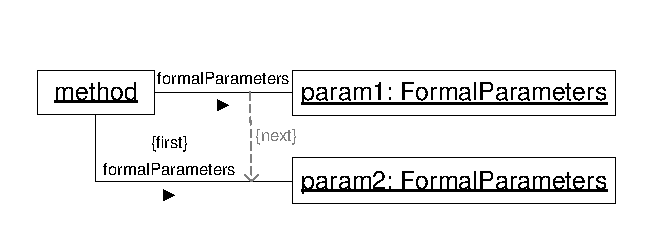
\includegraphics[width=0.75\columnwidth]{figures/LinkConstraintUnsatisfiablePattern}
\caption{Link Constraints causing a Story Pattern to be unsatisfiable.}
\label{fig:linkConstraintUnsatisfiablePattern}
\end{figure}

By supporting sequences of link order constraints (cf. Figure~\ref{fig:linkOrderConstraintDirectSuccessorCreateDelete}) and combinations of link position and link order constraints, we extend story patterns and their semantics as proposed by Tichy et. al.~\cite{TMG06}. The general semantical issue that the insertion into an ordered reference is non-deterministic remains, but may be explicitly solved using the link constraints introduced in this section. 

\begin{figure}[htb]
  \centering
  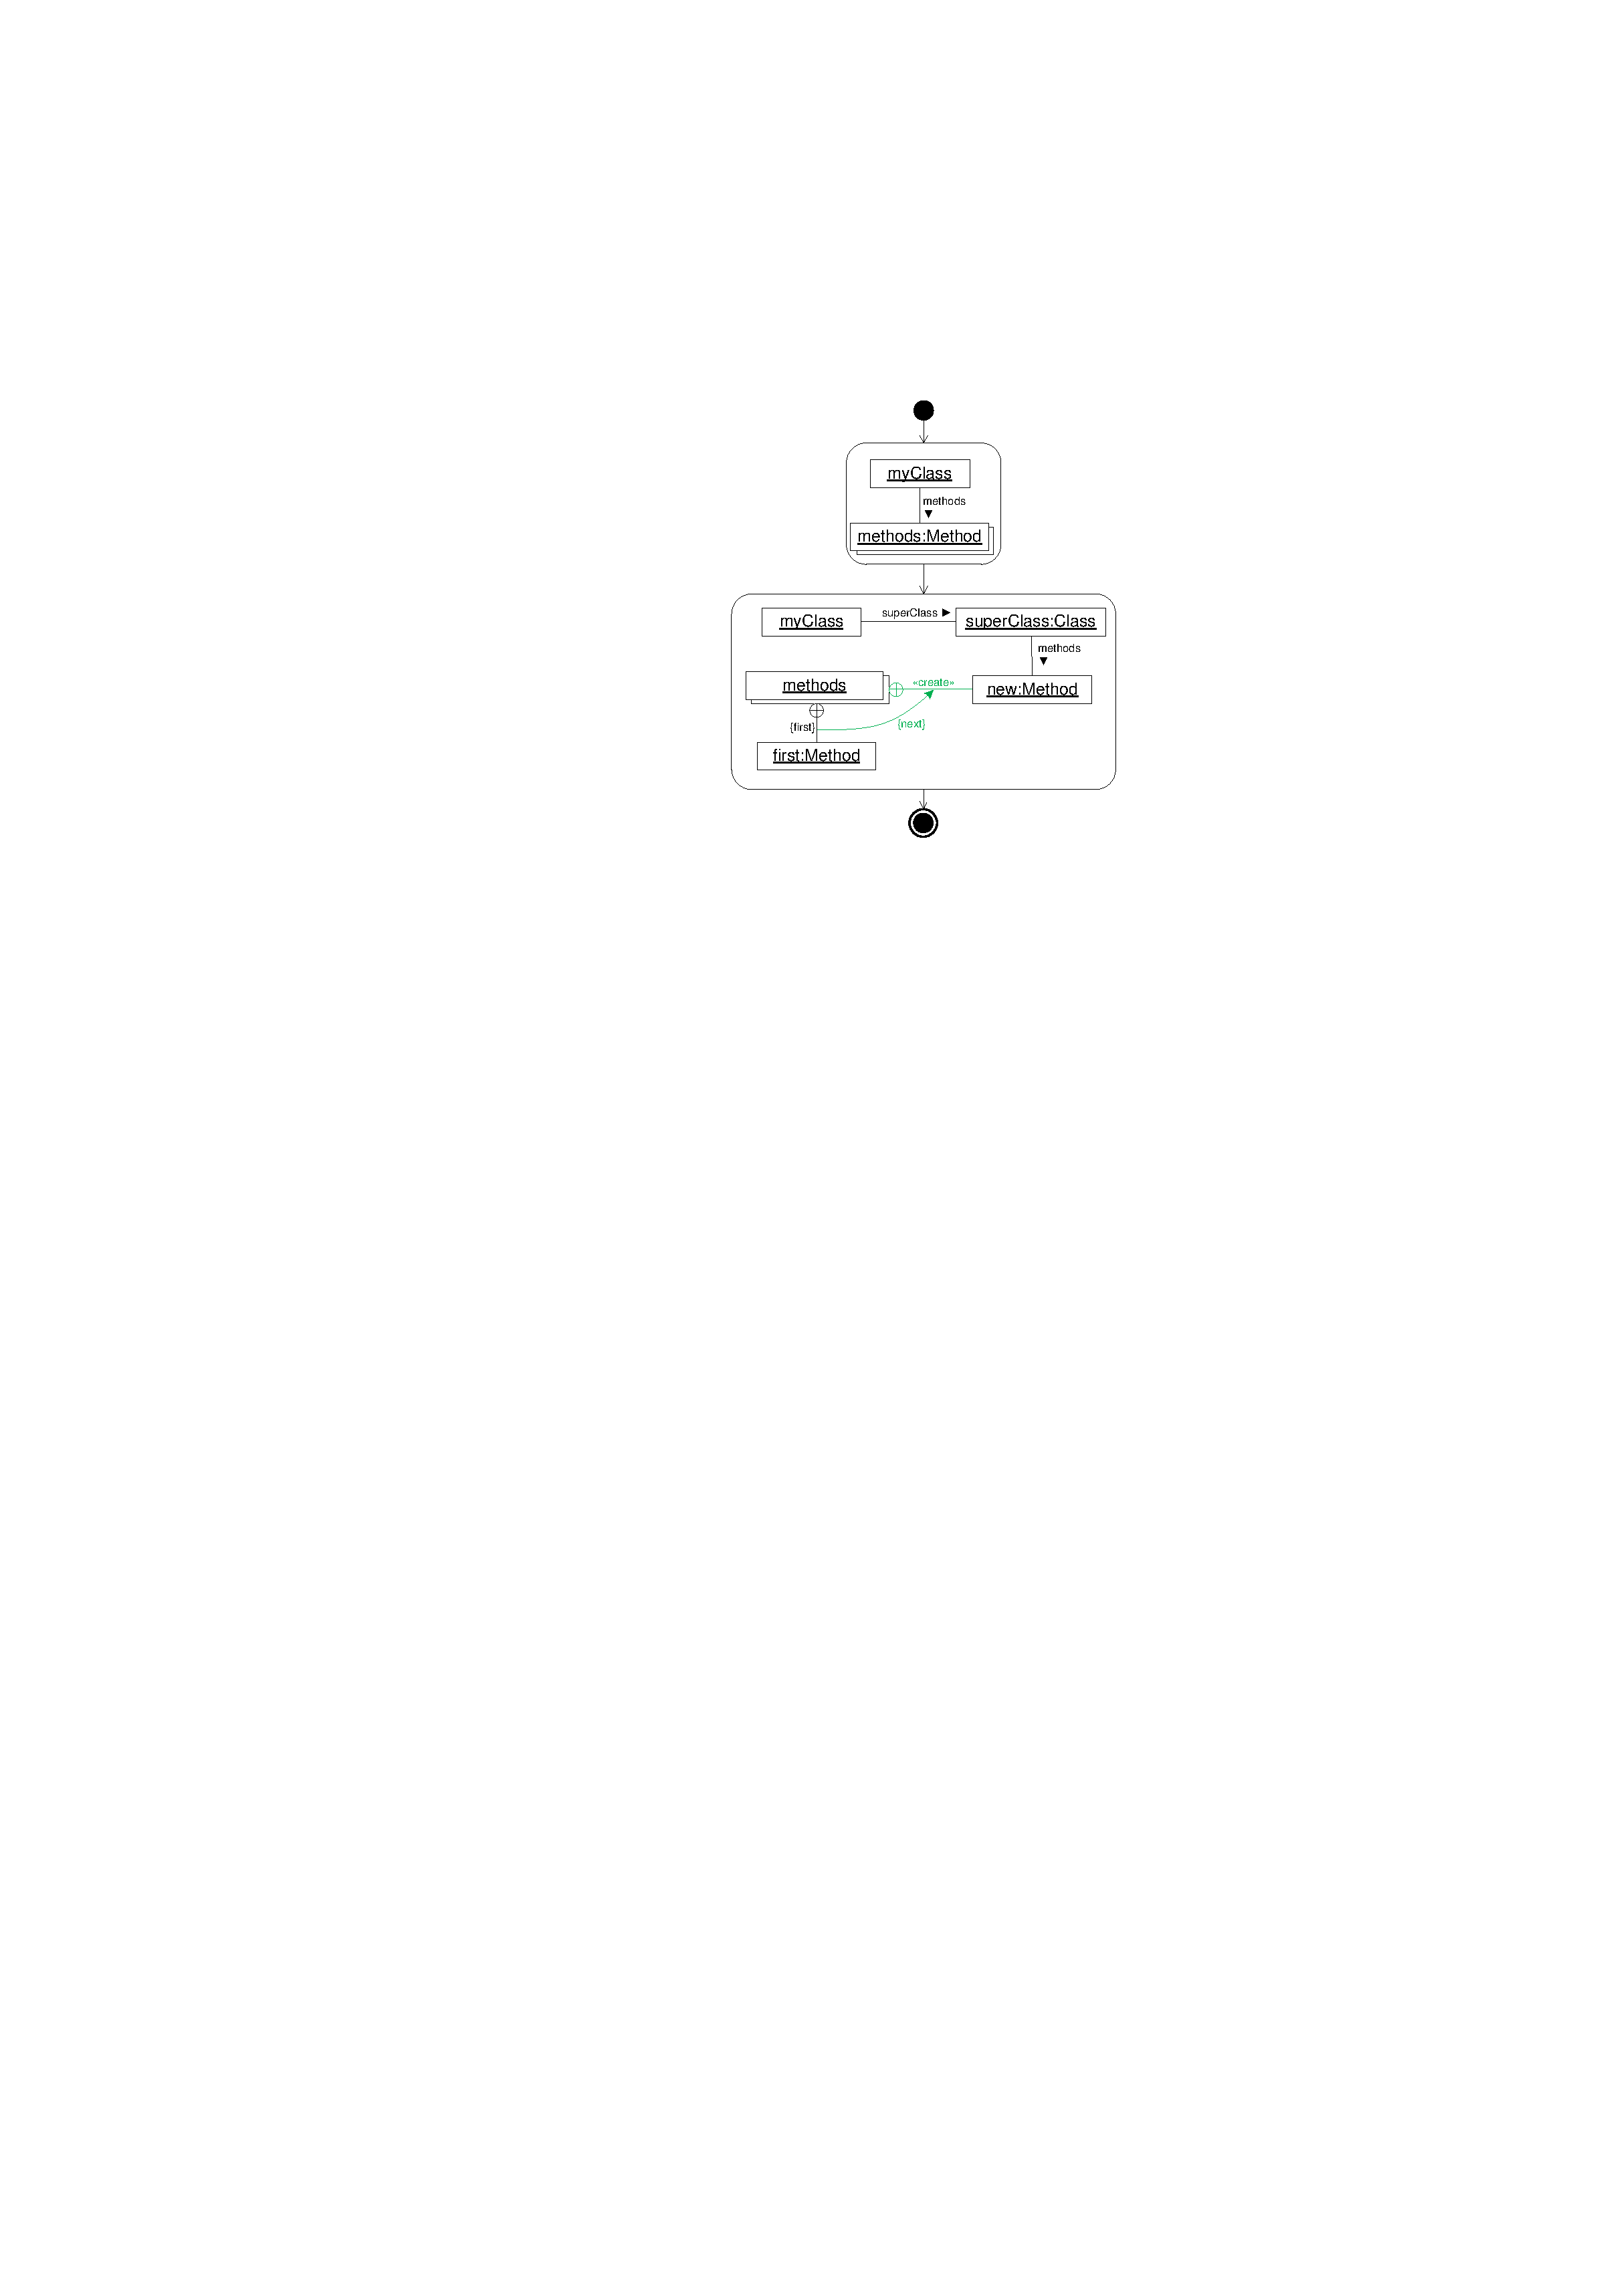
\includegraphics[scale=.8]{figures/LinkConstraints1}
  \caption{Inclusion Links With Link Constraints}
  \label{fig:collectionsLinkConstraints}
\end{figure}

Similar to the link constraints described in Section~\ref{sec:StoryPatterns:linkConstraints}, link constraints can also be used with inclusion links.
An exemplary use is illustrated in the story diagram in Figure~\ref{fig:collectionsLinkConstraints}.
We will explain story diagrams in more detail in Section~\ref{sec:StoryDiagrams}.
Here, the story diagram describes the sequential execution of two story patterns.

In the first story pattern (the upper one), a set of \fe{Method} objects is collected from a given class \fe{myClass} and stored in the collection \fe{methods}.
In the next story pattern, a superclass of \fe{myClass}, a method in this superclass and the first method in the collection \fe{methods} are matched.
In case of a successful matching the newly matched method \fe{new} is added to the collection \fe{methods}.
The link constraint \fe{\text\{next\text\}} determines to add this method to the ordered collection in such a way
that the method \fe{new} directly follows the method \fe{first} in the collection \fe{methods}.



} %--- End of link constraint subsection

\subsection{Maybe Links}
\label{sec:StoryPatterns:specialLinks:maybeLink}

Story patterns are matched by using isomorphic matchings. 
That means that two object variables in a story pattern may not be matched to the same object of the instance model. 
A matching which matches two object variables to the same object is, thus, considered to be invalid. 
In some situations, however, it should be explicitly allowed to match the same object to two different object variables inside the same story pattern. 
Then, the isomorphic matching must be disabled for the two corresponding object variables. 
This is achieved by connecting the object variables with a maybe link. 
Then, a matching \emph{may} assign the same object to the object variables connected by the maybe link, but it also may assign different objects to the variables.
For all other object variables, the isomorphism condition is enforced.


%\tododt{Please clarify the semantics of a \emph{maybe} link.
%It allows two object variables to be matched to the same object.
%For all aother variables an isomorphic matching is performed.
%I would also emphasize \emph{maybe}.}

\begin{figure}[htb]
  \centering
  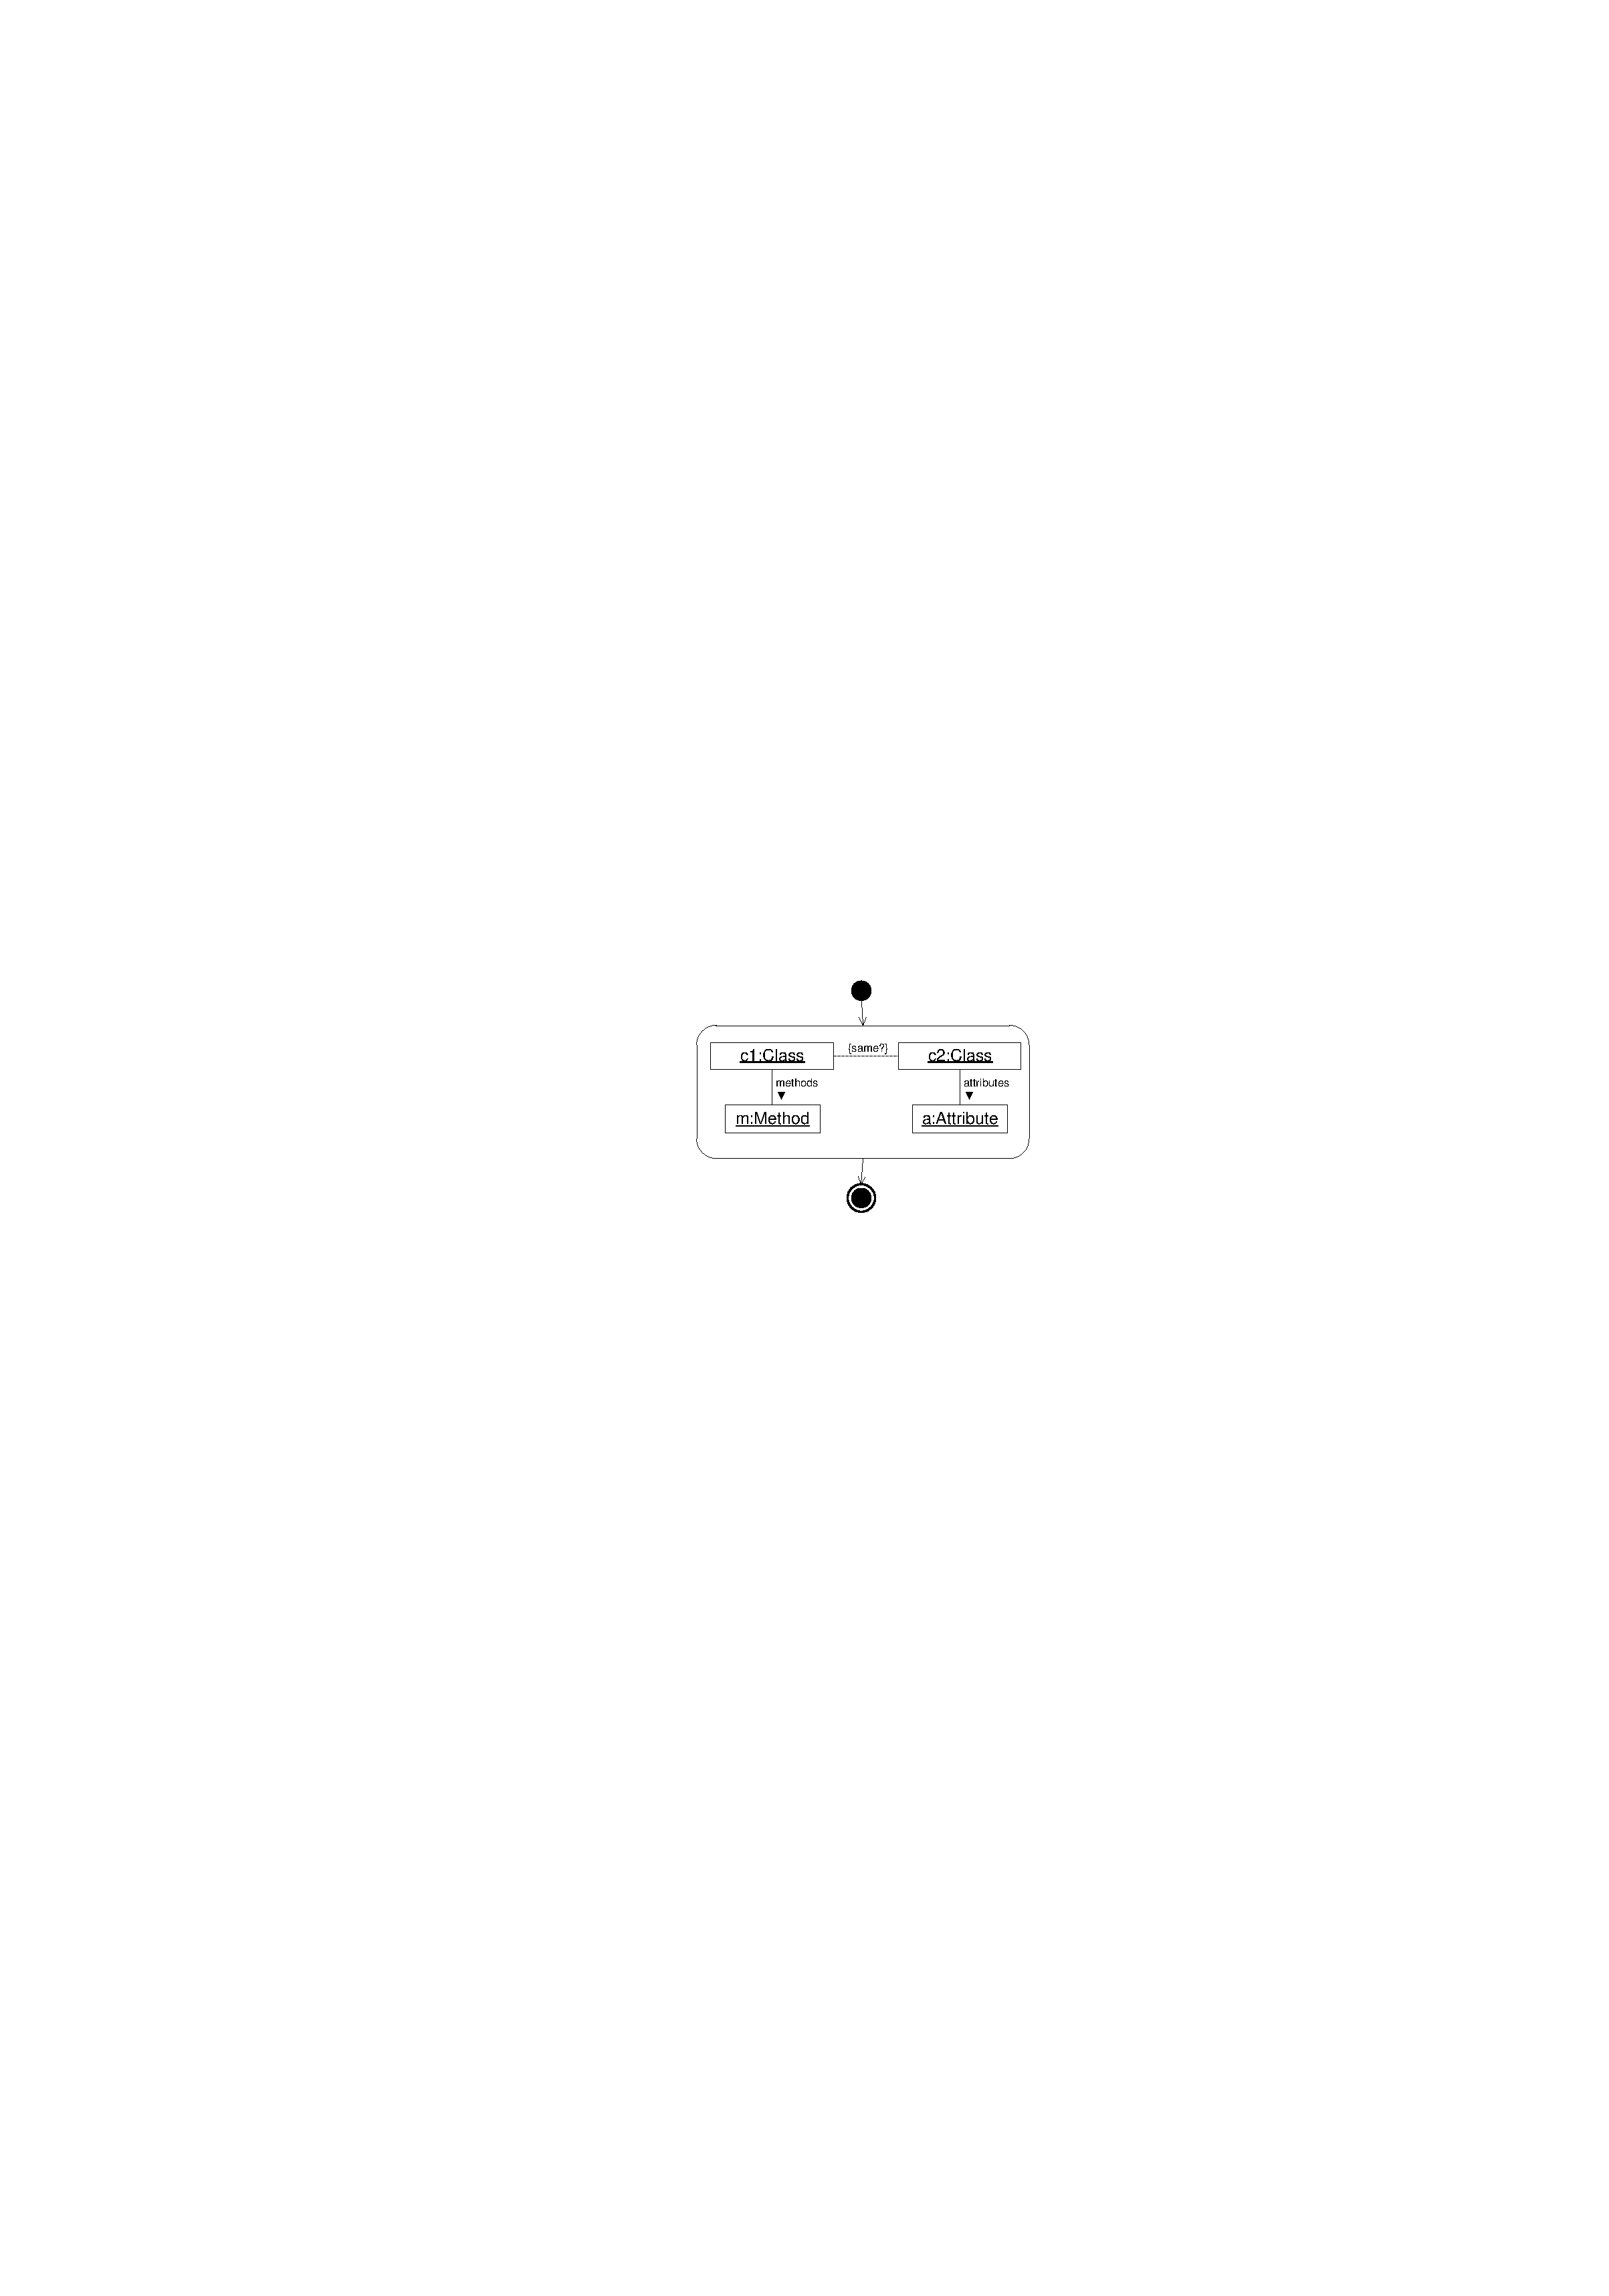
\includegraphics[scale=.8]{figures/MaybeLink}
  \caption{Maybe Link allowing two Object Variables to be matched to the same Object}
  \label{fig:maybeLink}
\end{figure}

Figure \ref{fig:maybeLink} shows the concrete syntax of maybe links. The object variables \fe{c1} and \fe{c2} are connected with a maybe link which is visualized by a dotted line labeled with \fe{\{same\}}.
The matching of the story patterns is successful if either two classes - one containing a method and one containing an attribute - can be matched in the instance graph \emph{or} if only one class containing a method \emph{and} an attribute can be matched.

If two object variables are connected by a maybe link, they both must be mandatory or optional. In addition, a maybe link requires the object variables to be matched or destroyed, but not created.  


%\ext  %--- Comment this line to include pattern constraints into the document
{
\subsection{Pattern Constraints}
\label{sec:PatternConstraints}

A pattern constraint defines an additional condition for a match that is evaluated and the end of the matching step, i.e., it is evaluated after all object and link variables have been matched. Since it is a condition, it needs to evaluate to true or false. If the pattern constraint is evaluated to true, then the match for the story pattern is valid. If the pattern constraint is evaluated to false, then the match is rejected.

A pattern constraint may use all object variables that are used in the same story pattern. Object variables are referred by their name. The pattern constraint may traverse the references of the objects bound to a particular object variable and access the attributes of the corresponding object. In the current version of story diagrams, we only support to use OCL for specifying pattern constraints. Then, the OCL constraint uses the name of the object variables to refer to objects and may use all features of OCL to access references and attributes of the corresponding objects.

\begin{figure}[htbp]
\center
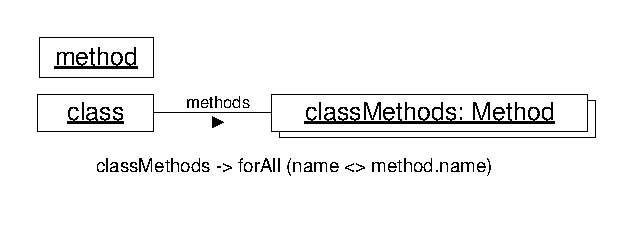
\includegraphics[width=0.6\columnwidth]{figures/PatternConstraint}
\caption{Example of a Pattern Constraint}
\label{fig:patternConstraint}
\end{figure}

\tododt{Should the constraint in Figure~\ref{fig:patternConstraint} not be classMethods->forAll(name <> method.name)? Otherwise the constraint does not check the matched methods in \fe{classMethods}.}

Figure~\ref{fig:patternConstraint} gives an example for the concrete syntax of a pattern constraint. The story pattern has two bound object variables \fe{class} and \fe{method} of types \fe{GASTClass} and \fe{Method}, respectively. The pattern constraint is visualized as a label containing the OCL constraint. In the example, the OCL constraints specifies that all methods of \fe{class} need to have a name which is different from the name of \fe{method}. In addition, the story pattern matches all methods of \fe{class} in the object set \fe{classMethods}. The matching of the story pattern is successful only if the pattern constraint is fulfilled.

} %--- End of pattern constraints section




\ext %--- Comment this line to include paths into the document
{ 
\subsection{Paths [MCP]}
\label{sec:StoryPatterns:paths}
} %--- End of paths subsection


\ext  %--- Comment this line to include pattern fragments into the document
{
\subsection{Pattern Fragments [MCP]}

patterns contained in other patterns, negative, semantics? review enhanced story patterns from Diss Florian Klein

\todomcp{Should contained pattern be marked as forEach? Idea for semantics: first the part of the pattern outside the forEach pattern is matched, then the forEach subpattern is applied to any match that may be located, the variables bound in a forEach subpattern may not be used in subsequent activities}

\todoch{The transformations diagrams that Matthias Meyer developed in his Diss contain so-called iterated parts that are essentially the same as a for-each fragment. We should check his semantics.}

\tododt{This is somewhat confusing.
As I understand them, subpatterns are ordinary story patterns within another story pattern.
They are surrounded by a fragment box and can be labeled with a name (see Figure~\ref{fig:labeledSubPattern}).
Special types of such subpatterns are negative application condition fragments (NACs), set fragments, and optional fragments.
As far as I know, we did not plan to add $\forall$ and $\exists$ fragments, did we?
These are only used in SDDs and TSSDs which are constraint languages.
}

\begin{figure}[htbp]
  \centering
  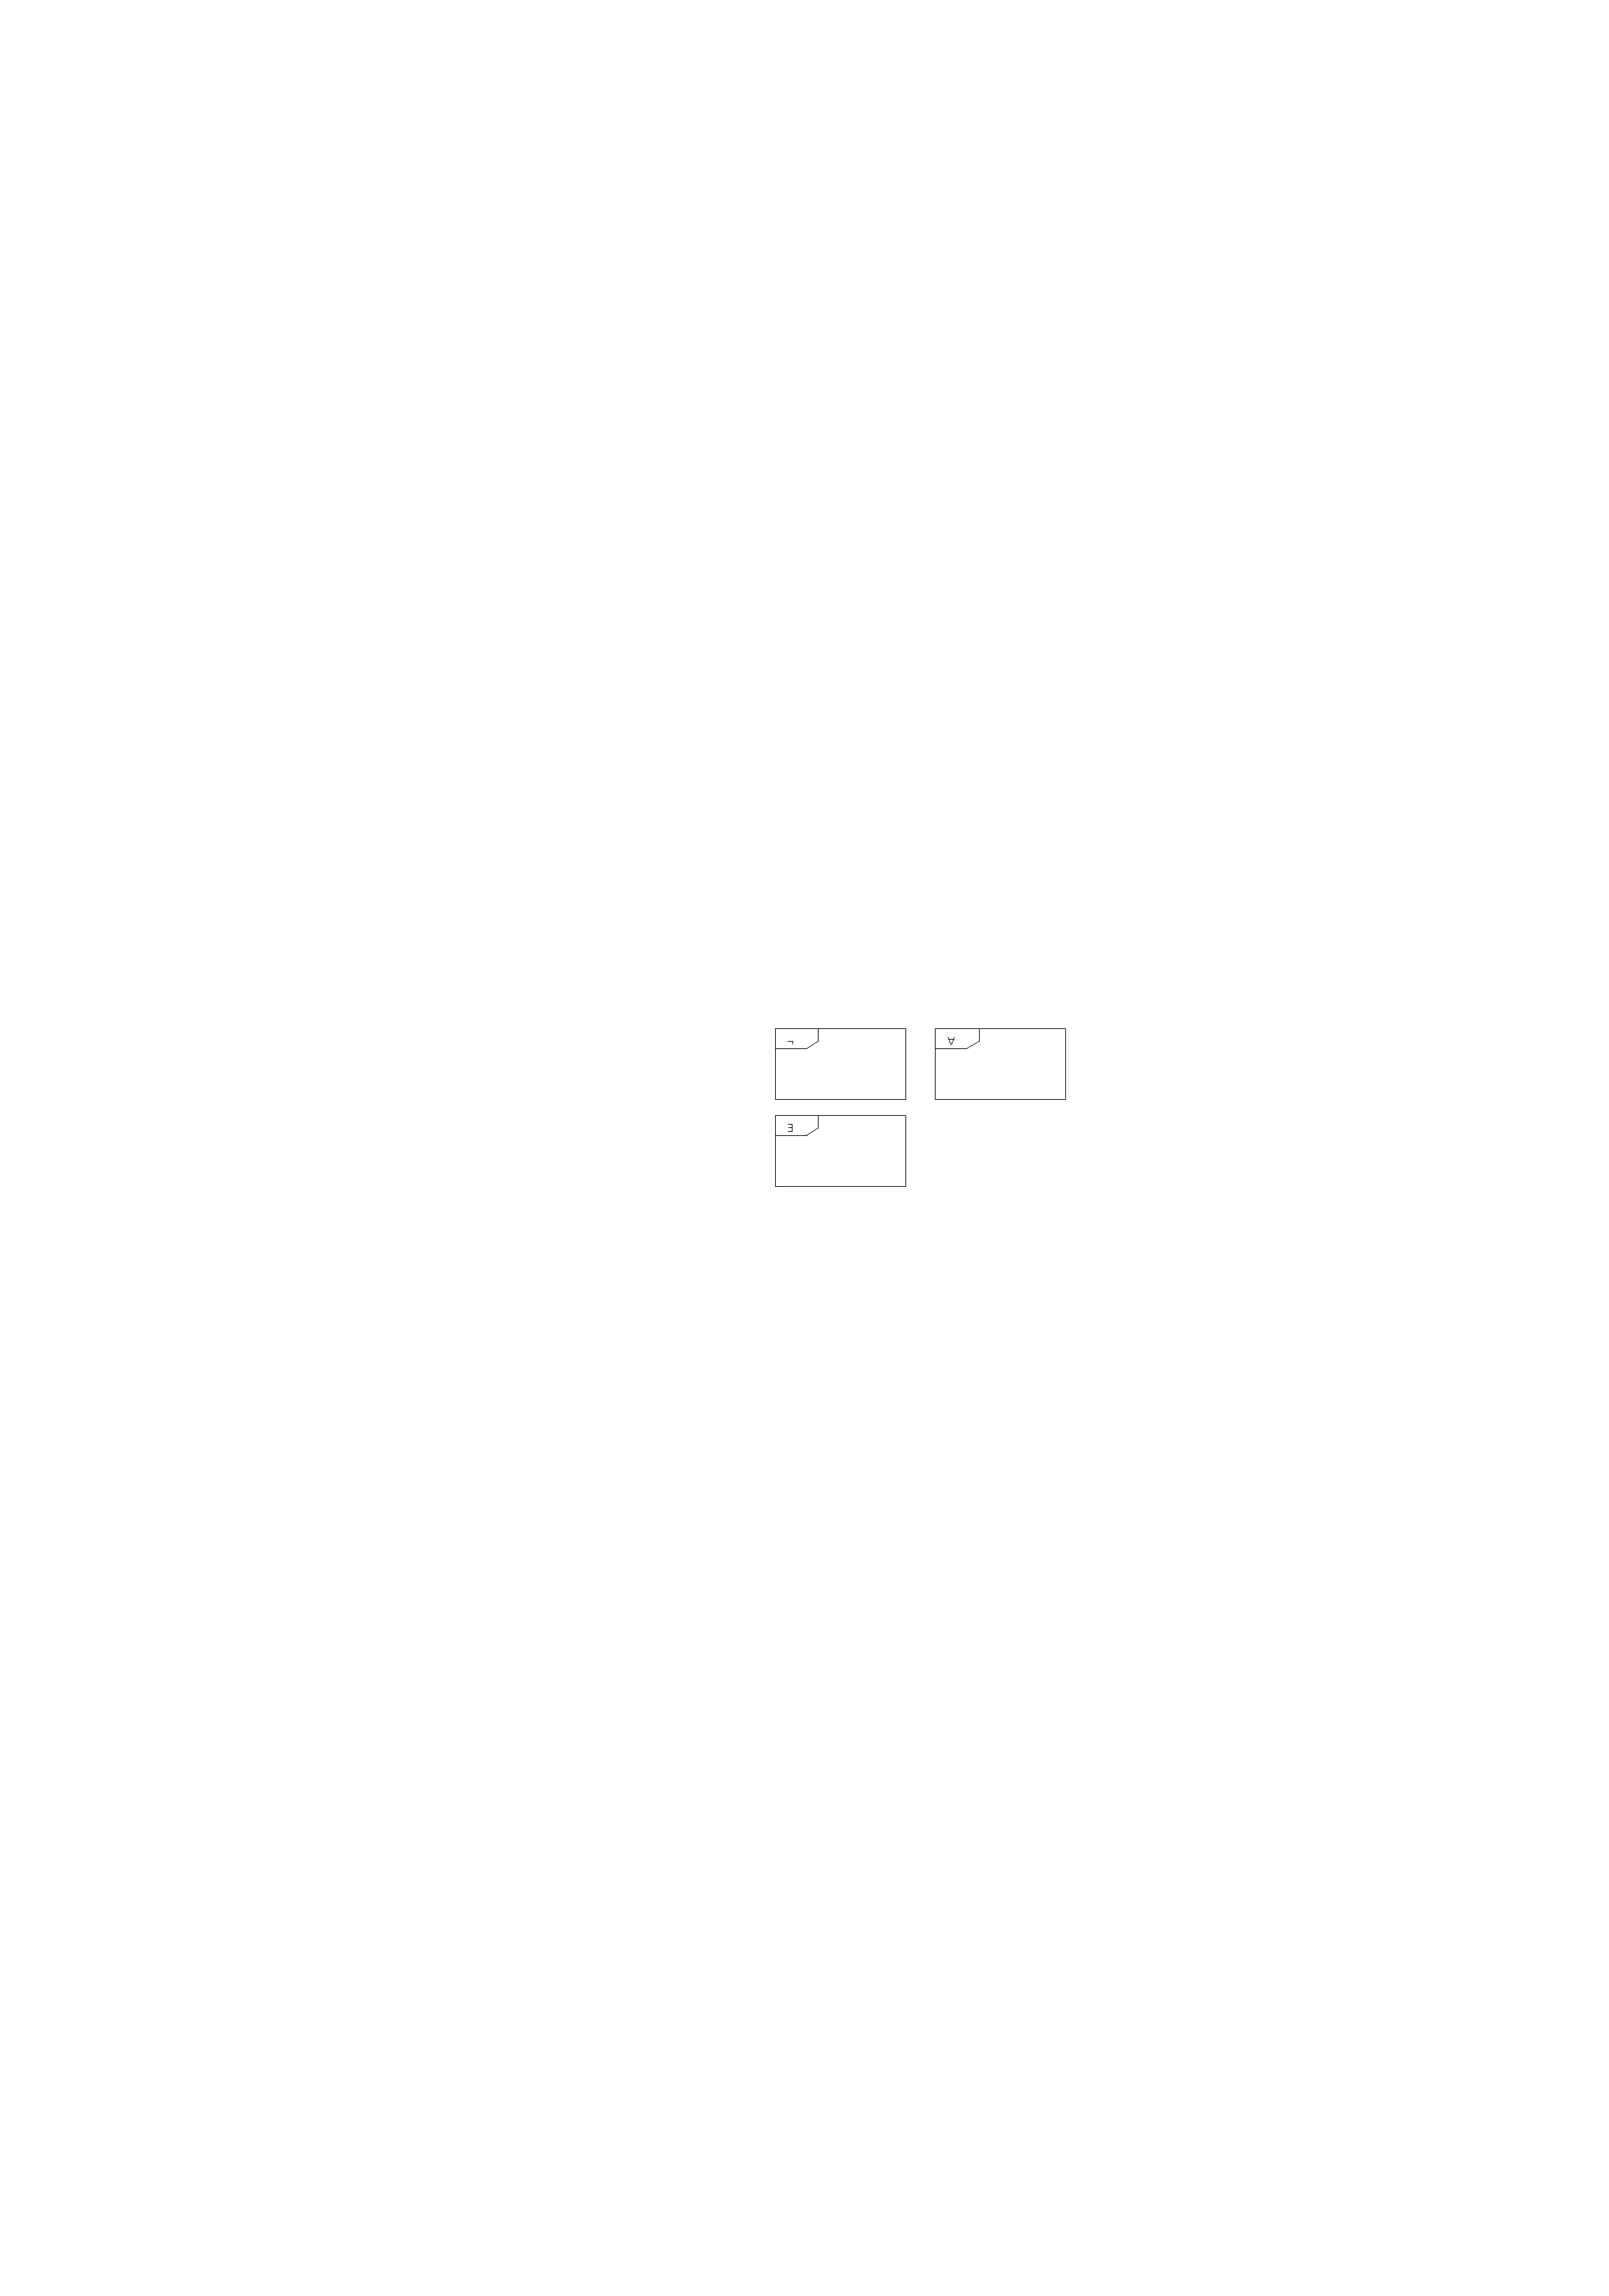
\includegraphics[scale=1.0]{figures/ContainedPattern}
  \caption{Different Kinds of Contained Patterns}
  \label{fig:containedPattern}
\end{figure}

\todomcp{Should contained pattern be marked as optional? Is currently possible in the metamodel. Idea for semantics: Whole pattern must be found, if found, variables may be used in subsequent activities, if pattern may not be found as a whole, matching still succeeds but all variables in the subpattern are not bound in subsequent activities.}
\tododt{I would say, contained patterns are mandatory in general (or are NAC/optional/set in case of the according fragment).}

\begin{figure}[htbp]
  \centering
  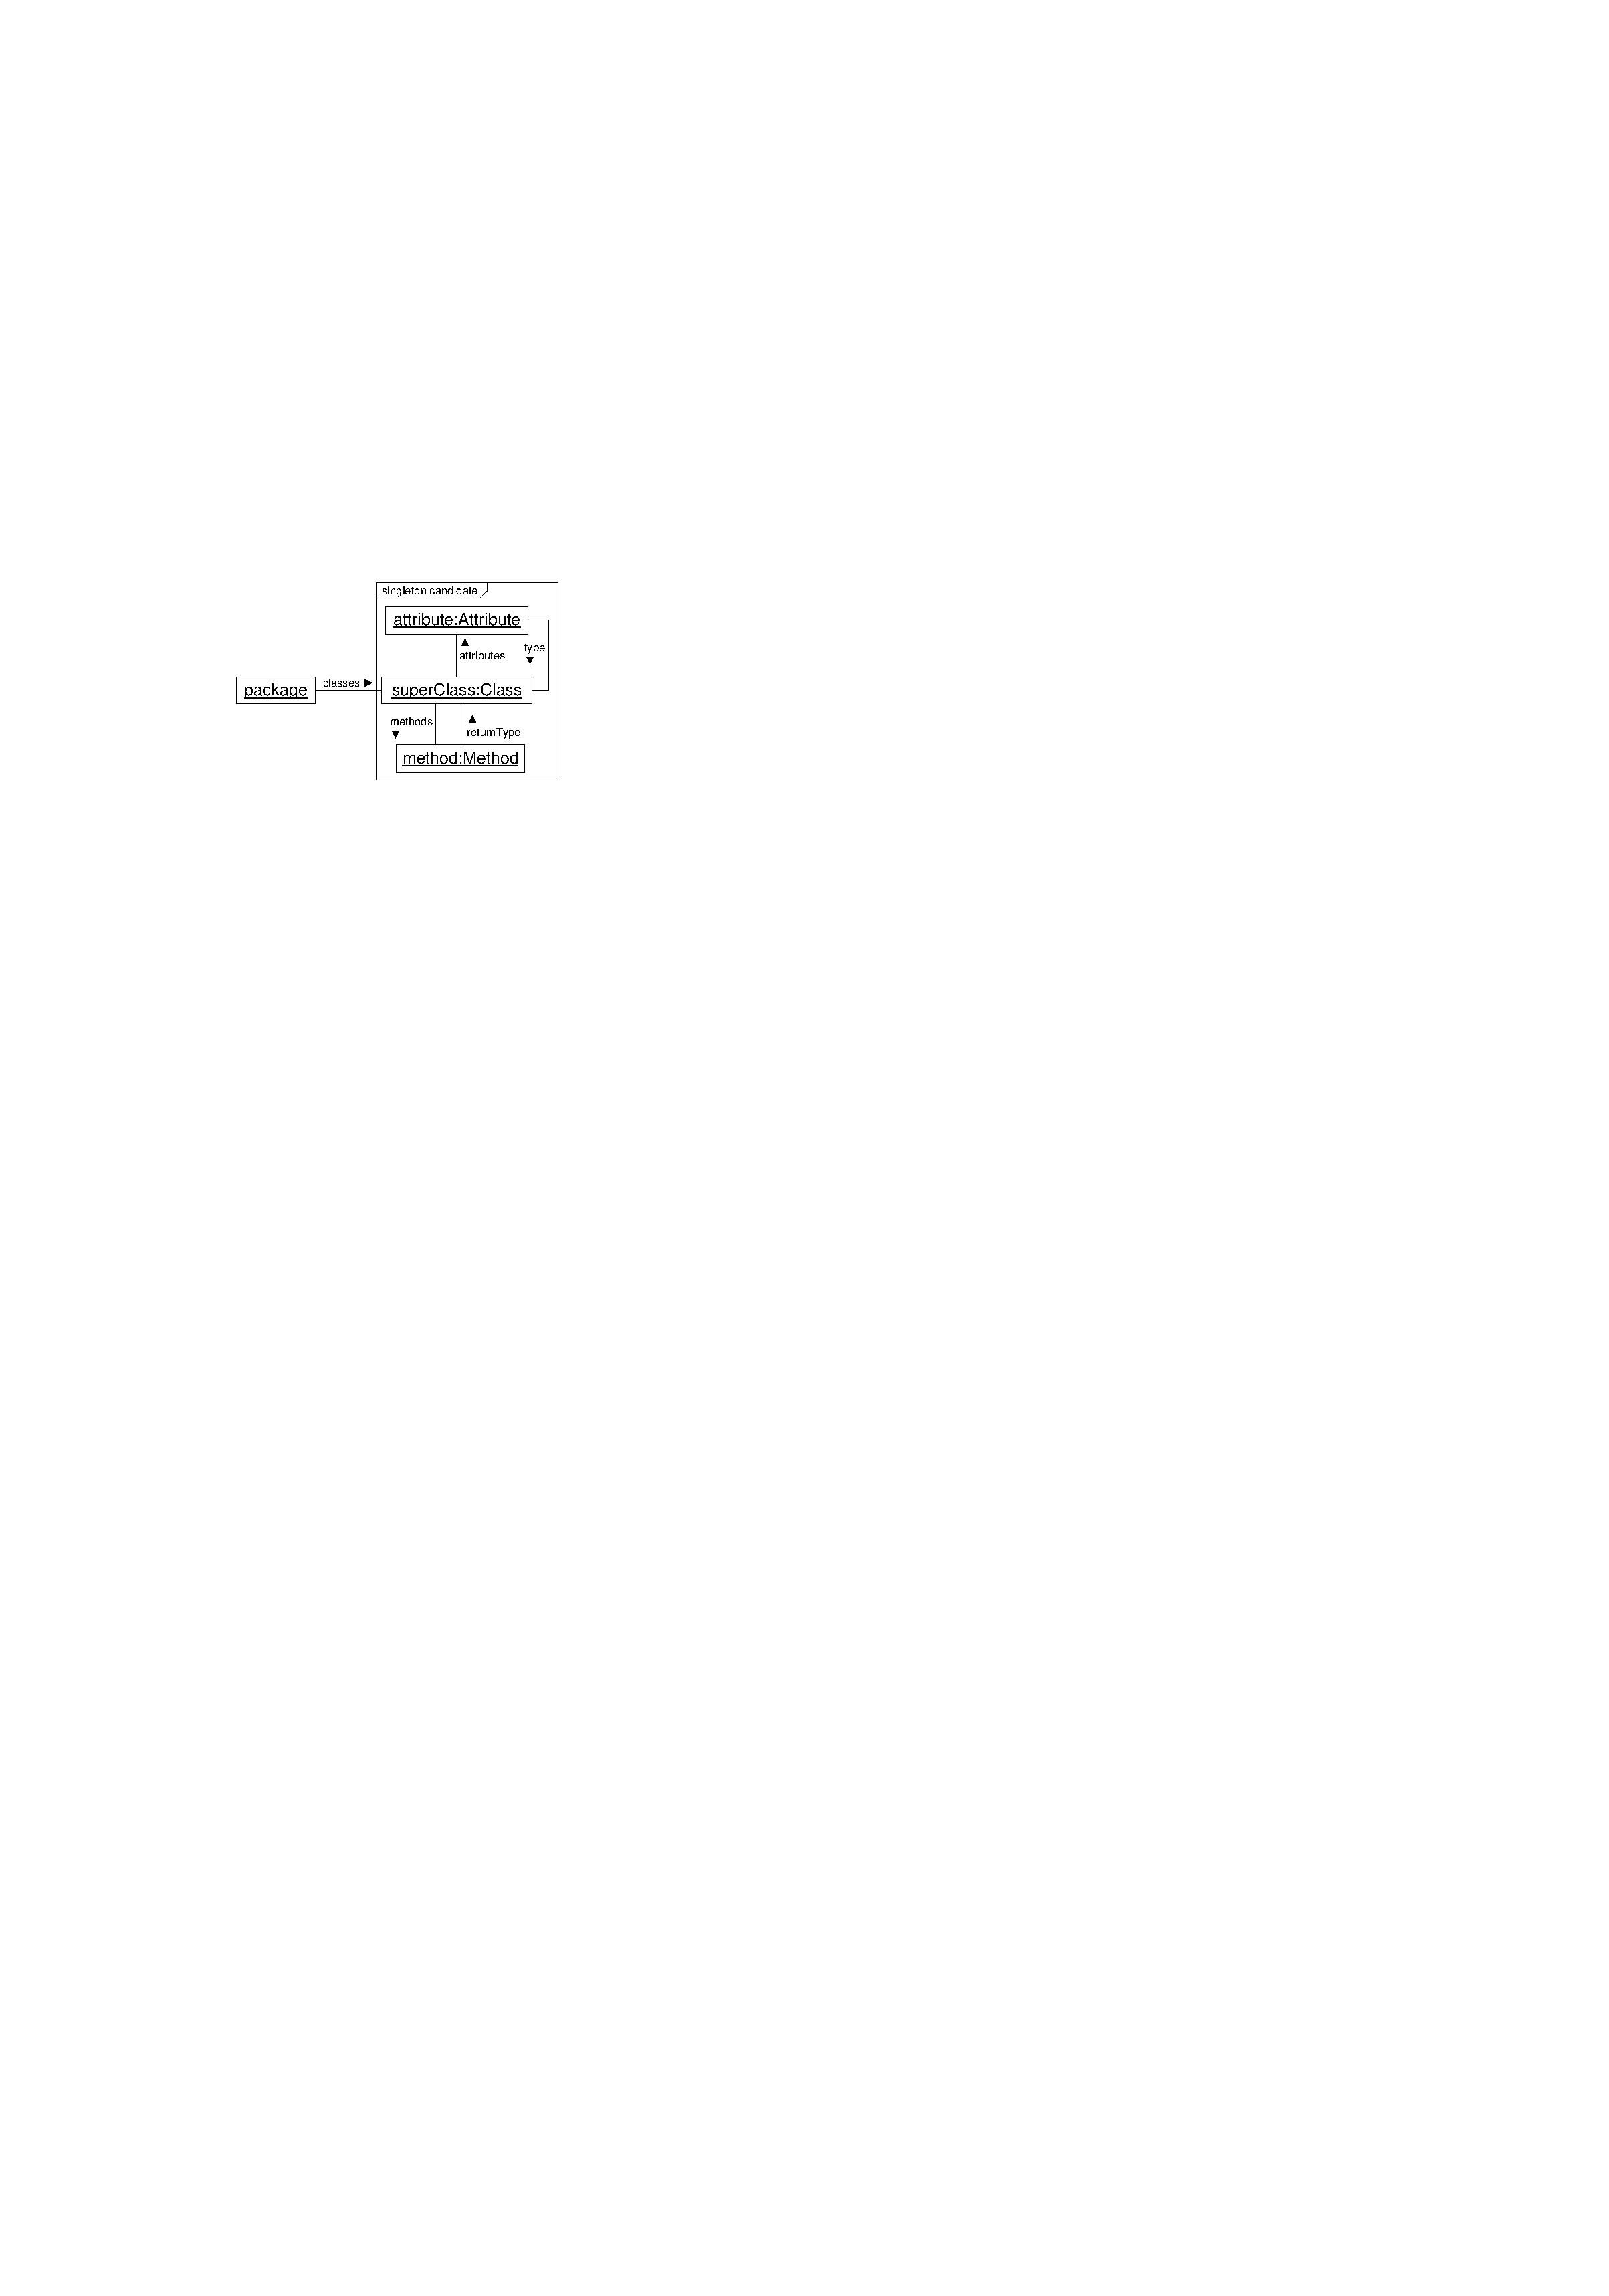
\includegraphics[scale=1.0]{figures/SubPatterns2}
  \caption{Labeled sub pattern}
  \label{fig:labeledSubPattern}
\end{figure}

\begin{figure}[htbp]
  \centering
  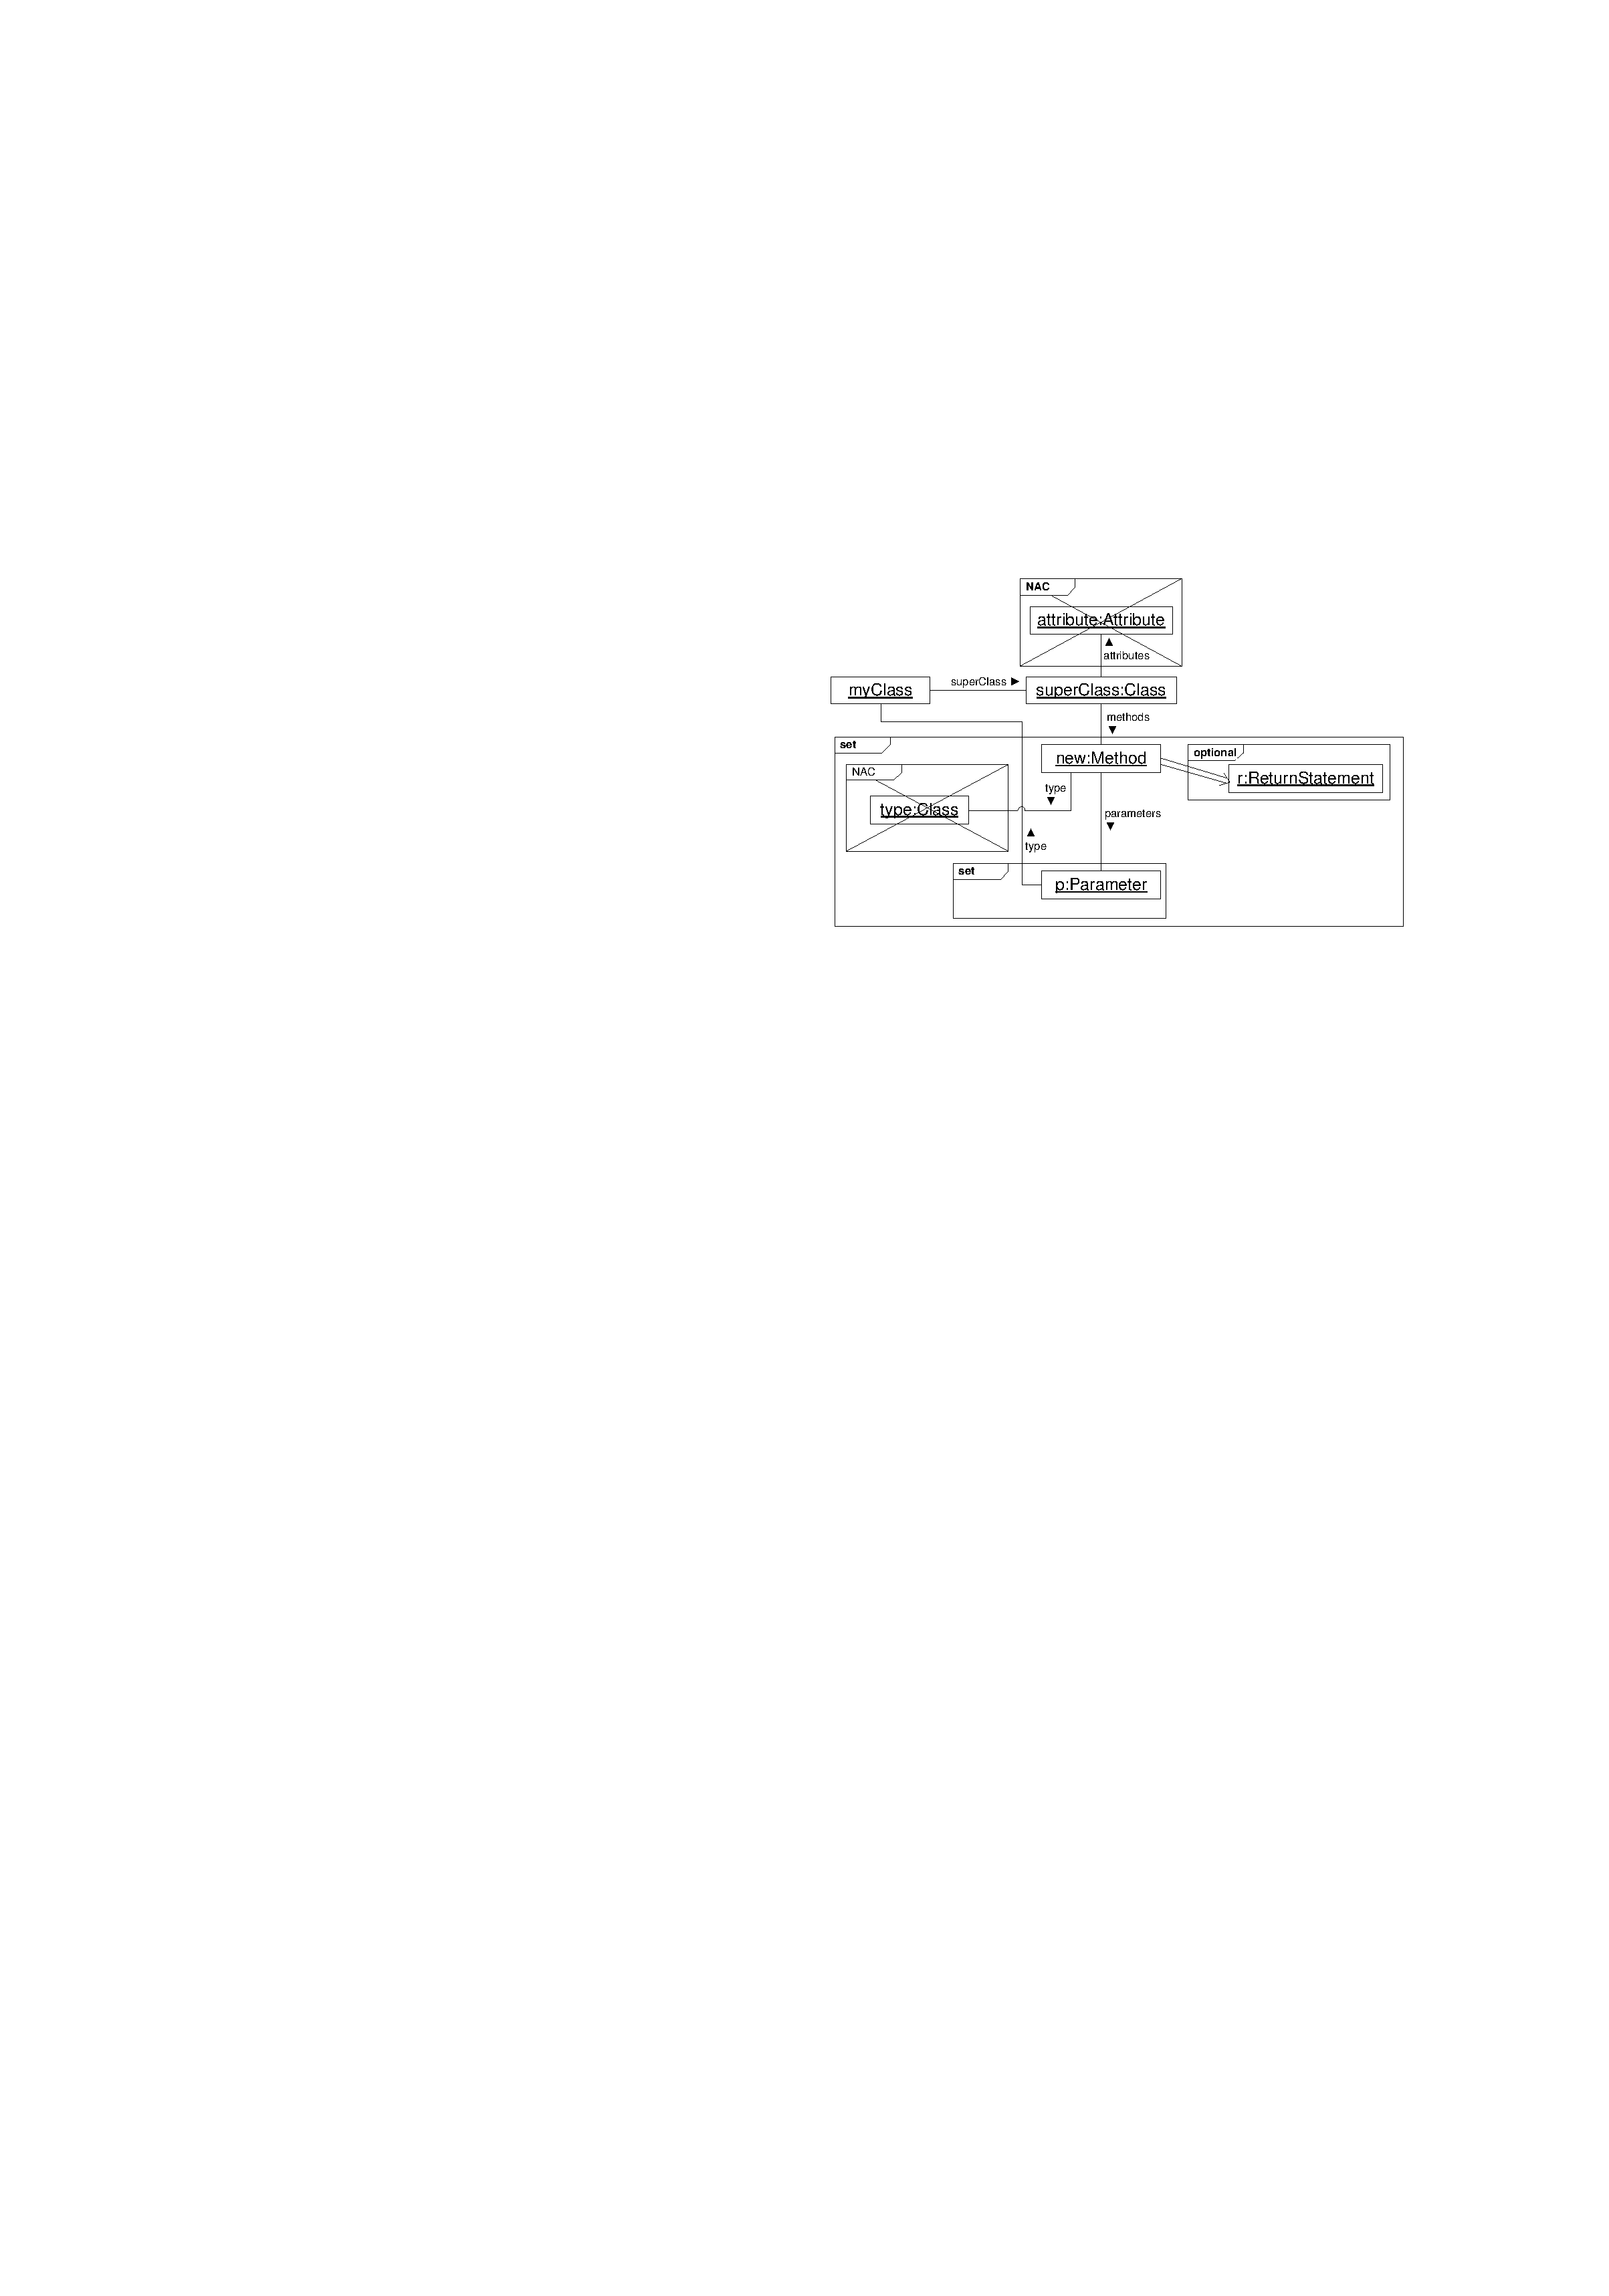
\includegraphics[scale=1.0]{figures/SubPatterns1}
  \caption{Hierarchies of NAC, set, and optional sub patterns}
  \label{fig:subPatternHierarchies}
\end{figure}

\todomcp{How deep may patterns be nested? What is the semantics of alternating binding semantics of sub-patterns, e.g., negative in optional in negative and so on.}
\tododt{I would prefer to allow arbitrarily deep nestings and would suggest to interpret the fragments in the order from outside to inside. Example (see Figure~\ref{fig:subPatternHierarchies}): You match a super class \emph{superClass} of \emph{myClass} and ensure that \emph{superClass} has no attribute. Then you you match all methods \emph{new} (outer set fragment) that have no class as their type (enclosed NAC fragment). Now you match for each of these methods all parameters (enclosed set fragment) that have \emph{myClass} as their type. Furthermore, you try to find a path from the matched \emph{new} method to a return statement (optional fragment).}

} %--- End of pattern fragment section


 
	
	\section{Story Diagrams} \label{sec:StoryDiagrams}

After explaining the concept of story patterns in Section~\ref{sec:StoryPatterns}, a prerequisite for this section, we explain the story diagrams themselves.
We give an overview of the general idea in Section~\ref{sec:IdeaStoryDiagrams} and go on with explaining the language constructs in the following sections.

\subsection{General Idea}\label{sec:IdeaStoryDiagrams}

% - combine activity diagrams and graph transformations as well as imperative, deterministic and declarative, non-deterministic languages to formally and compactly describe software behavior in terms of model transformations using an OO-based, familiar notation

The main idea behind story diagrams is to formalize UML activity diagrams
to better support model-driven software development.
This is done by not only modeling the software structure, but also completely modeling its behavior and, thus, making the software model executable.
For that purpose, graph transformations were chosen to formally specify behavior and have been combined with UML activity diagrams.
The result, story diagrams, is a mixture of two languages:
an imperative, deterministic language for the description of control flow, namely UML activity diagrams,
and a declarative, non-deterministic, object-oriented, graph-transformation-based language for the description of model modifications, so-called story patterns (see Section~\ref{sec:StoryPatterns}).
Both languages are graphical, formally defined, and use a familiar notation based on UML 1.5 activity diagrams\footnote{Actually,
we use the notation of UML 1.5 activity diagrams, but already use the terminology of the UML 2.}
and UML object diagrams with minor modifications.

An exemplary story diagram is illustrated in Figure~\ref{fig:simpleStoryDiagram}.
This story diagram takes a graph-based representation (a model of a so-called abstract syntax graph, see Section~\ref{sec:typeGraph}) of an object-oriented program, e.g., in Java,
and replaces calls of a given method (\fe{oldMethod}) with calls of another given method (\fe{newMethod}).

\begin{figure}[htb]
  \centering
  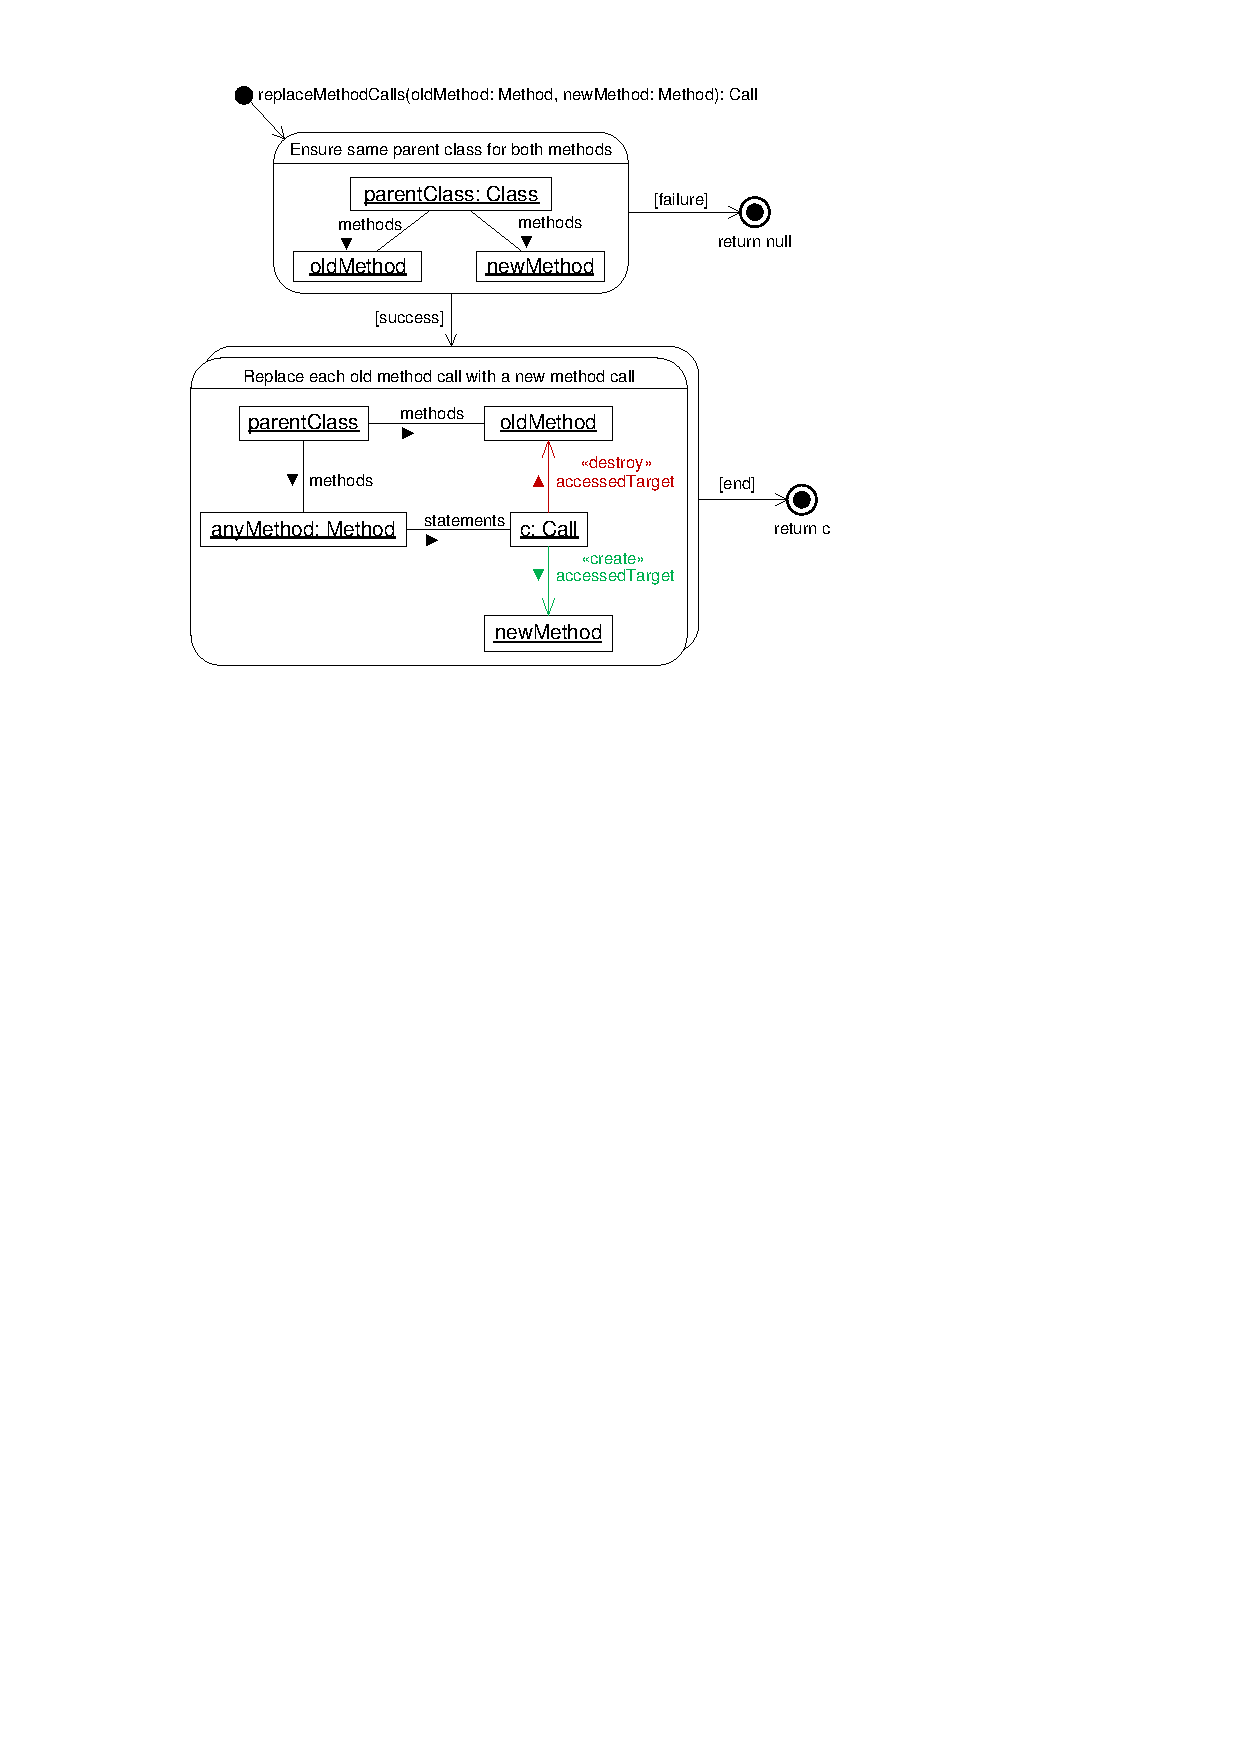
\includegraphics[scale=1.0]{figures/SimpleStoryDiagramExample}
  \caption{Exemplary Story Diagram -- Replace Method Calls}
  \label{fig:simpleStoryDiagram}
\end{figure}

Like UML activity diagrams, story diagrams model control flow by means of activity nodes and activity edges.
Each activity node embeds a story pattern to formally specify the behavior for this node\footnote{There are
some exceptions like activity call nodes which do not contain story patterns to specify the behavior.}.
The activity edges can carry guards.
These are either specified by boolean expressions, e.g., checking attribute values of a matched object,
or by keywords used to specify decisions on whether a story pattern could be
matched or not\footnote{A story pattern is successfully matched if for each object and link variable in the pattern corresponding objects and links are found in the instance model (host graph) and all specified constraints are satisfied.}.
In Figure~\ref{fig:simpleStoryDiagram}, the used guards are \fe{\text[success\text]} (successful execution of a story pattern),
\fe{\text[failure\text]} (failed to completely execute a story pattern),
and \fe{\text[end\text]} (activity edge points to the first activity node to be executed after a loop).

In contrast to ordinary UML activity diagrams, story diagrams, so far, do not model concurrent execution.
Thus, the language constructs \emph{fork} and \emph{join} are currently not supported in story diagrams.
We plan to include these concepts in future versions of story diagrams.

%- Story diagrams in MDSD process, 2 worlds: stand-alone transformations and specifications of methods' behavior:
%  1. alternative (completely modeling software): model classes in class diagrams, specify their methods' behavior in story diagrams, generate executable source code (e.g. Java) or use an interpreter
%  2. alternative (specify recurring model operations/transformations for a given type of models): model only classes representing the editor's model under development (meta-model), specify modification operations of this model (adding and removing elements, analysis operations, translations to/generation of other models, etc.), need of a software that triggers the specified operations, the operations can be performed using generated code or an interpreter
%- introduce an example

Basically, there are two different ways of using story diagrams in a model-driven software development process.

Originally, story diagrams were used in object-oriented software development to formally specify the behavior of methods that are defined in classes.
Calling such a method means to execute the story diagram that represents the method's behavior.
If there is a story diagram that models the behavior for each method specified in a class model,
the software model completely covers the software's structure and behavior and, thus, can be analyzed and executed.
In this case, story diagrams specify the behavior of objects whose properties are defined by classes.
For that reason, those story diagrams have a \emph{this} variable -- similar to the keyword \emph{this} in Java -- representing the object (a class instance) that they belong to (a self reference).
This variable can be used as a starting point for the graph matching specified in a story diagram.

For example, the class diagram in Figure~\ref{fig:SDWithThisClassDiagram} defines a method \fe{findAttribute} for all \fe{Class} objects.
This method's behavior is specified by the story diagram in Figure~\ref{fig:SDWithThis}.
The matching of the object structure specified in the contained story pattern, in this case,
starts with the \fe{this} object variable of the type \fe{Class} which is already bound
to the \fe{Class} object that the \fe{findAttribute} method belongs to.
Thus, this method tries to find an attribute \fe{a} in the same class with the name given by the method's parameter \fe{text}.

\begin{figure}[htb]
	\centering
  \begin{minipage}[t]{.4\textwidth}
    \centering
    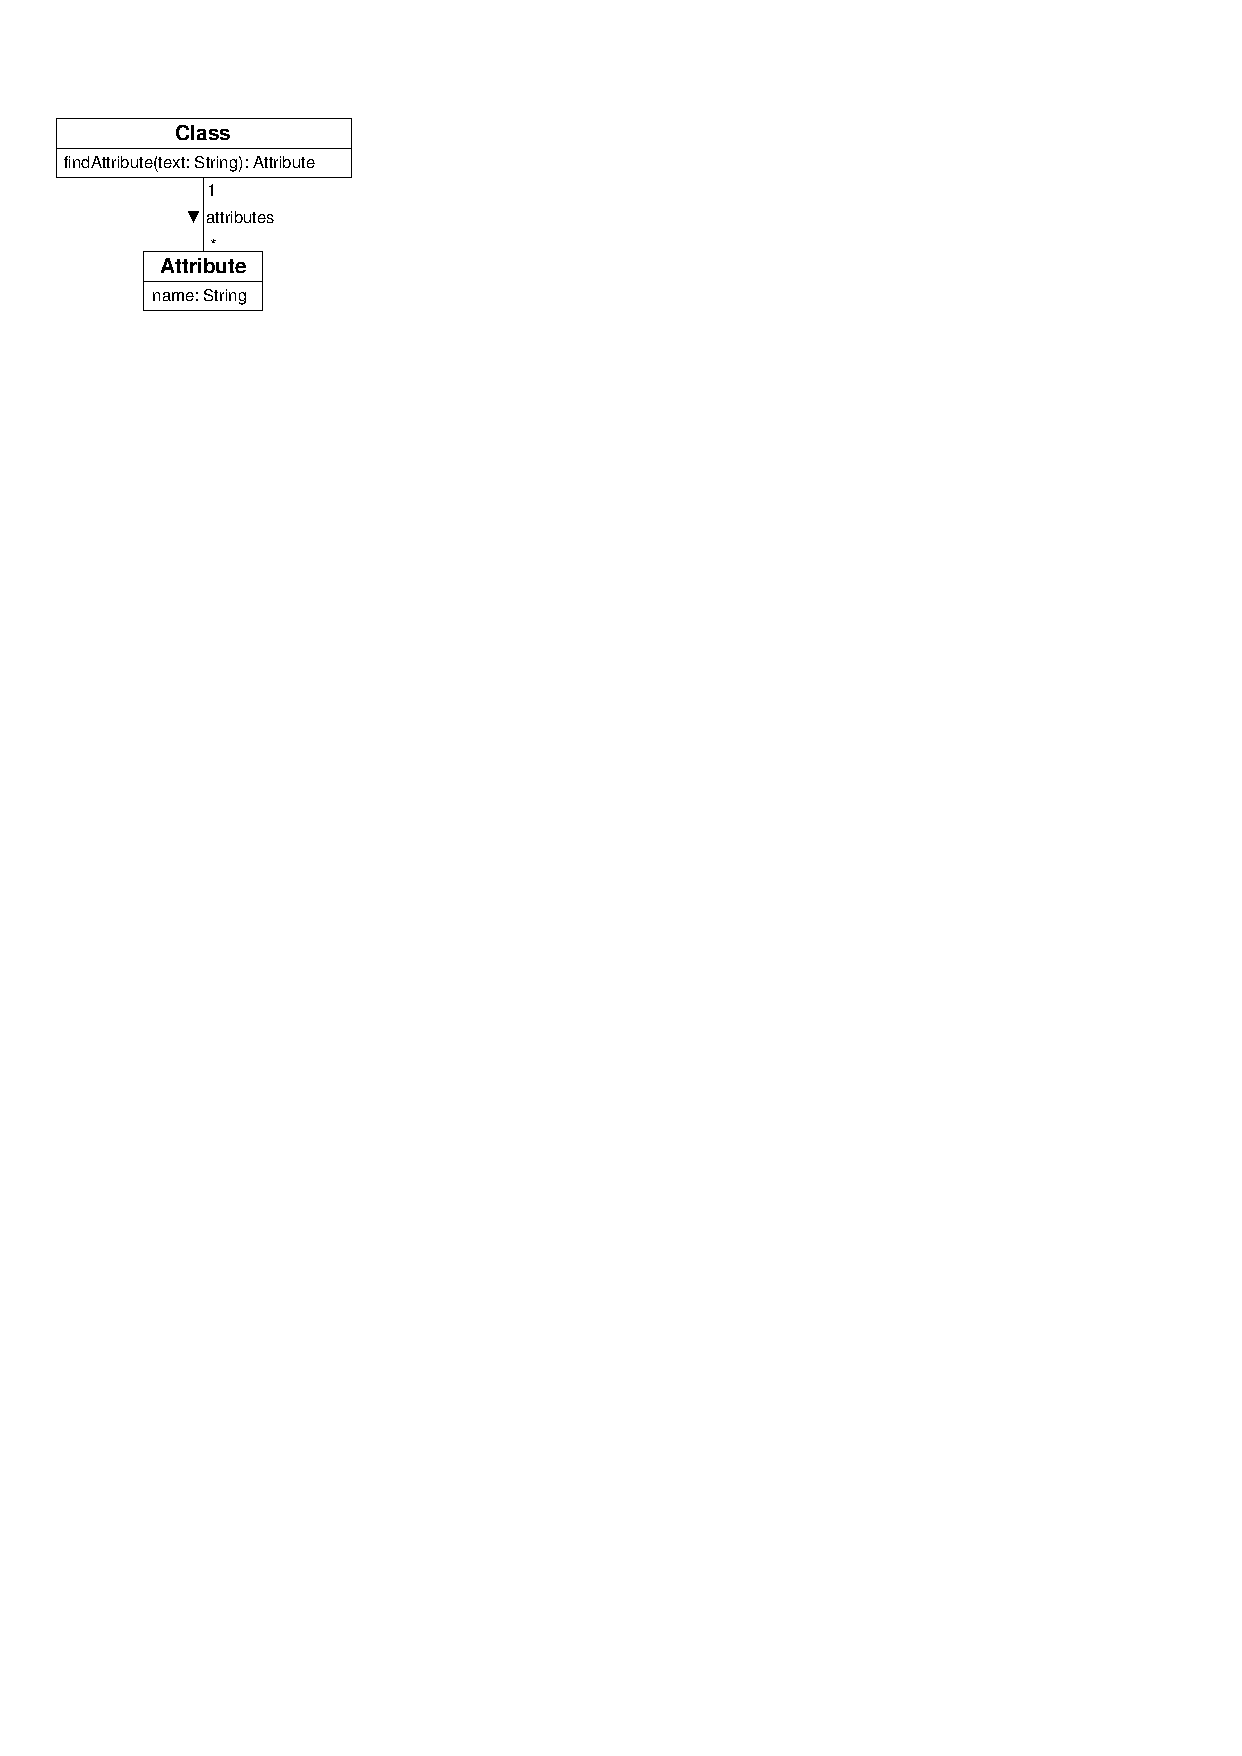
\includegraphics[scale=1]{SimpleSDFindAttributeClassDiagram} 
    \caption{Type Model for the Story Diagram in Figure~\ref{fig:SDWithThis}}
    \label{fig:SDWithThisClassDiagram}
  \end{minipage}%
  \hfill
  \begin{minipage}[t]{.55\textwidth}
    \centering
    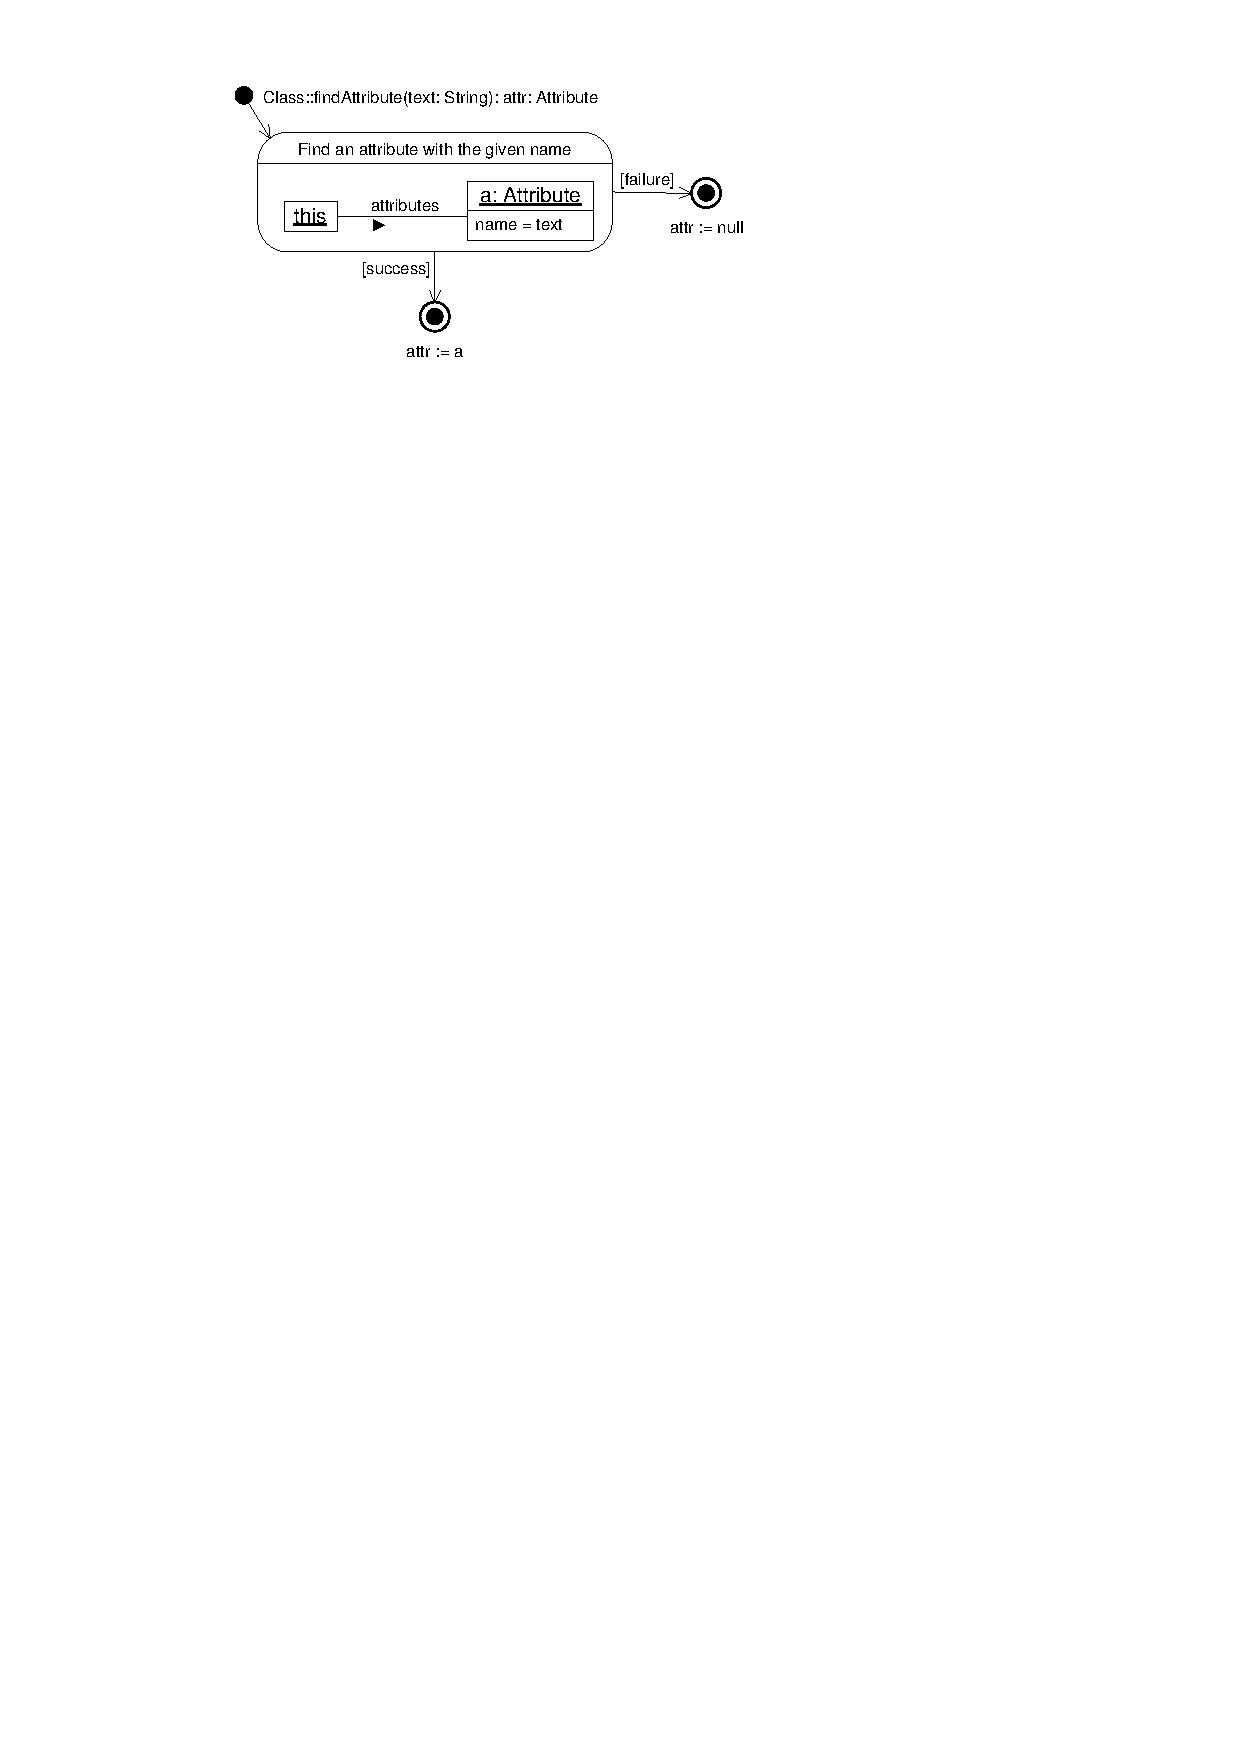
\includegraphics[scale=1]{SimpleSDFindAttribute}
    \caption{Exemplary Story Diagram With \emph{this} Object Variable}
    \label{fig:SDWithThis}
  \end{minipage}
\end{figure}

\begin{figure}[htb]
	\centering
  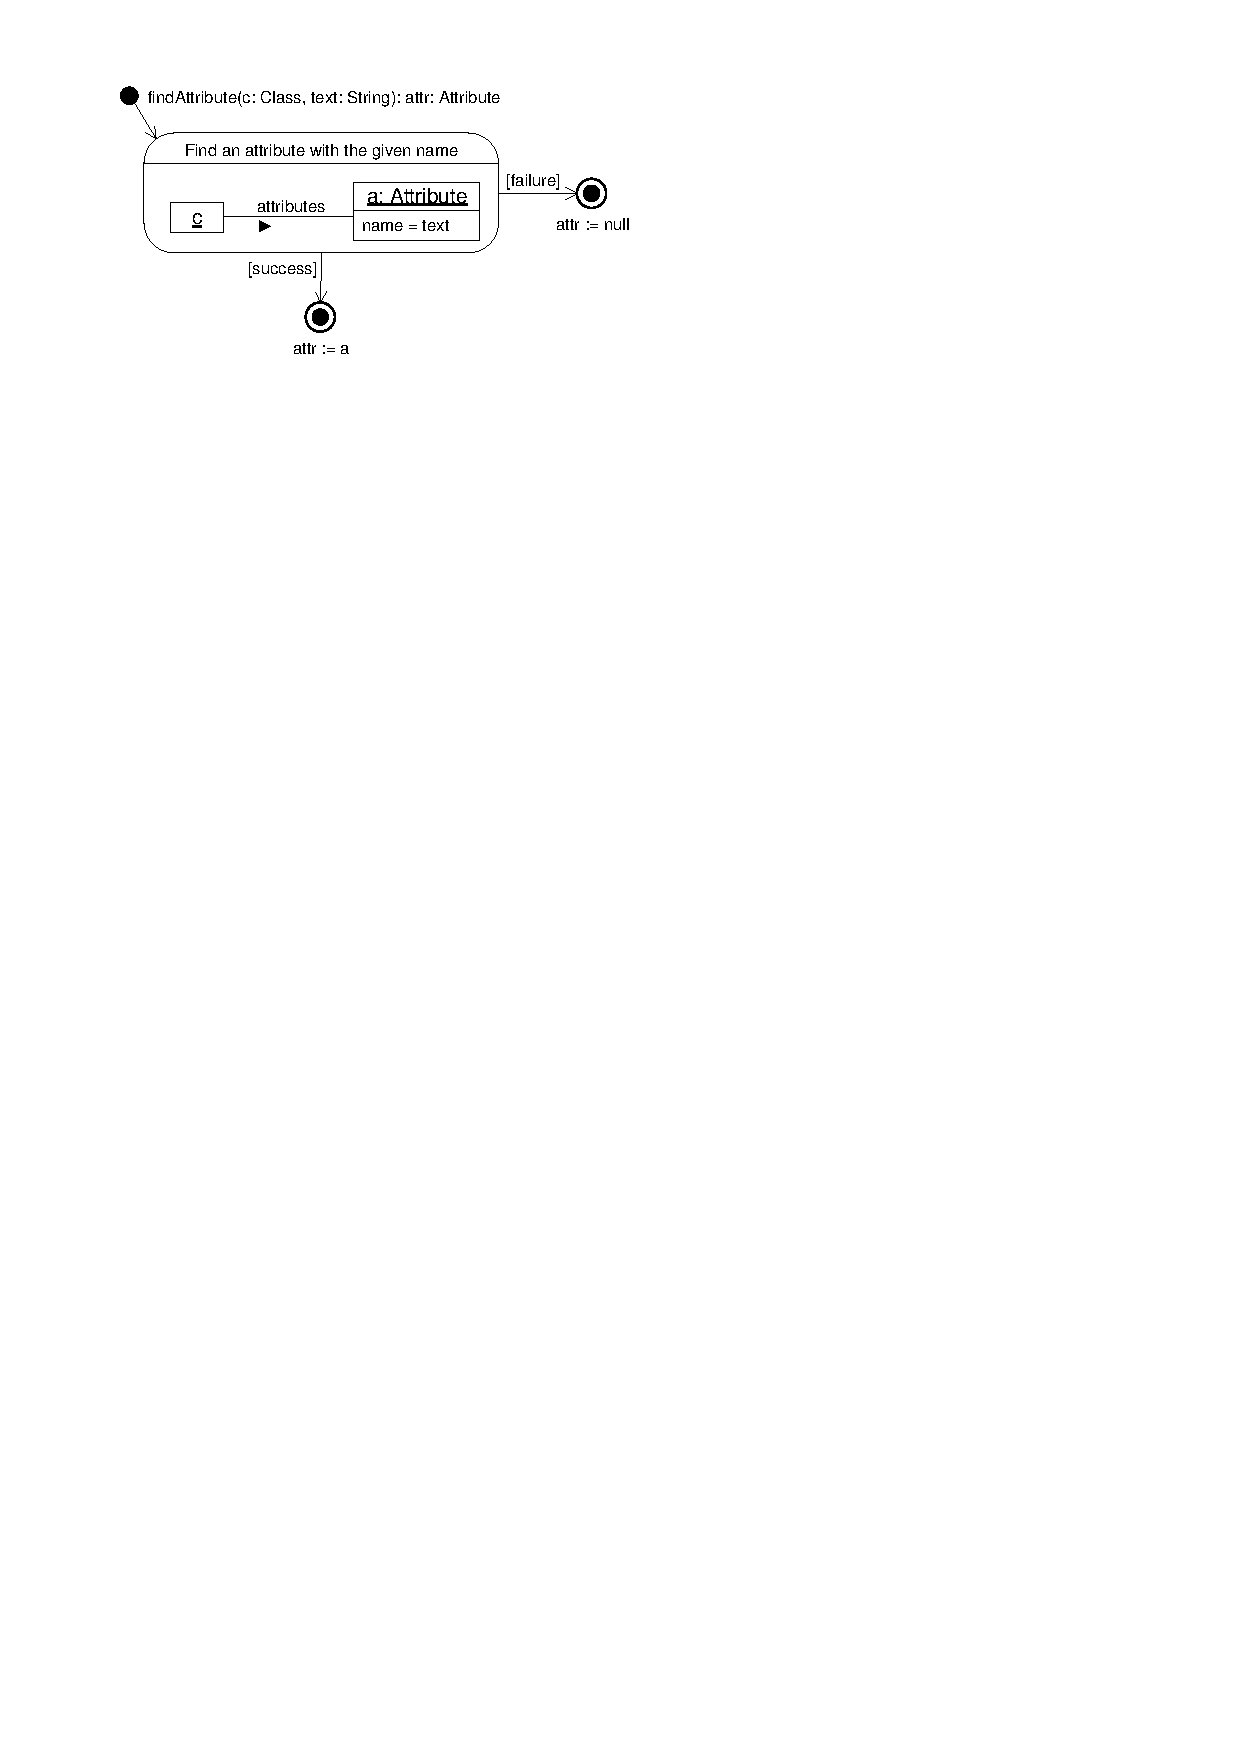
\includegraphics[scale=1]{SimpleSDFindAttributeStatic} 
  \caption{Exemplary Story Diagram Without \emph{this} Object Variable}
  \label{fig:SDWithThisStatic}
\end{figure}

Another more flexible way of using story diagrams is to specify any kind of model transformation or operation in a story diagram without attaching this behavior to a certain class.
In contrast to the previous case, there is no \emph{this} variable that could be used as a starting point for the graph matching.
All starting nodes for the graph matching have to be provided as arguments of the story diagram call.
For this purpose, in contrast to the story diagram in Figure~\ref{fig:SDWithThis}, the story diagram in Figure~\ref{fig:SDWithThisStatic} has an additional parameter \fe{c}.
The corresponding arguments of a story diagram call are assumed to be known (bound object variables) and are used as starting points for the graph matching.
This way, the operations or transformations defined by story diagrams can be used from within any other part of the developed software, like a software library would be used.
Typically, model-to-model transformations, consistency checks, or more generally speaking, recurring and object-independent operations are defined this way.

% - enable formal analyses to check/ensure certain behavioral software properties

In both cases, story diagrams can be used to generate executable source code or be executed using an interpreter.
Besides execution, the formally defined story diagrams can also be analyzed to guarantee certain behavioral properties \cite{Mey09,Zue09}.
For example, model checking can be used to check whether a certain invariant holds
(e.g.\ that all accessible variables are still accessible after a refactoring operation)
or if a critical state can ever be reached (e.g.\ if an attribute or method has no parent class after a refactoring operation which would result in an incorrect program).

A complete description of the story diagrams' abstract syntax is given in the Appendix~\ref{sec-reference}.
There is also a grammar that determines all feasible story diagrams by constraining their structure.
The latest version of this grammar can be found in Thomas Klein's diploma thesis \cite{Kle99}.


%\subsection{The Language Constructs in Story Diagrams (Jan/Dietrich)}\label{sec:StoryDiagrams:composition}

\subsection{Activities, Activity Parameters and Return Values}\label{sec:activities}

Since story diagrams can be seen as special UML activity diagrams, we reused the class names defined by the UML 2.
Thus, similar to UML activity diagrams, a story diagram is represented by a so-called activity (class \fe{Activity}).

Each story diagram can have parameters.
We distinguish \emph{in} and \emph{out} parameters,
i.e.\ parameters representing arguments given when a story diagram is called (\emph{in})
and parameters representing return values (\emph{out}).
Parameters are either \emph{in} or \emph{out} parameters.
%Parameters can be \emph{in} and \emph{out} parameters at the same time.
The story diagram in Figure~\ref{fig:SDWithThisStatic} has two \emph{in} parameters \fe{c} and \fe{text}
as well as an \emph{out} parameter \fe{attr} of the type \fe{Attribute}.
If there are more than one \emph{out} parameter, these are comma-separated.

If a story diagram defines the behavior of a method, the parameters are defined by the corresponding method's signature.
In this case, the number of \emph{out} parameters is limited to one single parameter and represents the only \emph{return} value of the method and story diagram.
Besides these parameters, there is another implicitly defined parameter \fe{this}
which -- similar to Java's \fe{this} keyword -- represents the object that the story diagram belongs to.

In case a story diagram is not defining a method's behavior, it defines its own signature explicitly with according \emph{in} and \emph{out} parameters.
The number of \emph{out} parameters is allowed to be arbitrary in this case and there is no \emph{this} parameter.

The values or objects returned after execution of a story diagram are defined by expressions in the \emph{stop} activity nodes.
For example, the object matched to the object variable \fe{a} is returned by the story diagram in Figure~\ref{fig:SDWithThisStatic} in case of a successful execution.
This is specified by the expression \fe{attr := a} which represents an assignment of the value of object variable \fe{a} to the \emph{out} parameter \fe{attr}.
Otherwise, an empty reference is returned which is specified by the keyword \fe{null}.
This notation is taken from Matthias Meyer \cite{Mey09}.

\subsection{Activity Nodes, Activity Edges} 
\label{sec:storydiagrams:activitynodes}

A story diagram's control flow is defined by activity nodes and activity edges, similar to UML activities.
Except for the cases where an activity node represents a call of another story diagram,
each node embeds a story pattern to specify the corresponding behavior.
Such activity nodes are called \emph{story nodes}.
Executing a story node results in executing the embedded story pattern.

In contrast to single story patterns, story patterns contained in story nodes of a story diagram have a different scope.
Here, you can reuse all object variables declared in the story patterns of preceding story nodes.
For example, in Figure~\ref{fig:simpleStoryDiagram} (p.~\pageref{fig:simpleStoryDiagram}),
the object variable \fe{parentClass} is reused in the second story pattern
by specifying the variable as a bound variable, i.e.\ the variable does not have to be matched anymore.

Executing a story node means executing the corresponding story pattern
which, in turn, means finding a subgraph with the specified properties
(e.g.\ finding objects of a certain type, with certain attribute values, and with certain connections)
and performing specified modifications of the found subgraph
(e.g.\ creating or removing objects and links or changing their attribute values).

We distinguish two kinds of story nodes: \emph{modifying story nodes} and \emph{matching story nodes}.
A matching story node contains a story pattern that only matches a specified object structure, but does not change it.
A modifying story node also performs modifications of the matched object structure.
For static analyses of model transformations described with story diagrams,
it is helpful to know which transformations do not modify the instance model.

\subsection{Activity Final Nodes} \label{sec:StopNodes}

The application of a story diagram can succeed or fail.
Usually, when the matchings are successful and the specified transformations can be carried out, the story diagram is considered to be applied successfully.
When a matching is unsuccessful somewhere or something unforeseen happens and the application has to be aborted, the story diagram's application is considered to have failed.
This is comparable to a method call either returning a desired result or returning false or null if something goes wrong.

\tododt{I would remove or replace this first paragraph.
In my opinion, the success and failure of story diagrams are not necessarily dependent on the success or failure of some pattern matchings or transformations in the same story diagram.
In Figure~\ref{fig:successAndFailureStopNodes} one could also model that the story diagram is considered to be successfully executed if the matching in the first story pattern fails.
Thus, success or failure of a story diagram is used like an implicitly declared boolean out parameter describing if the operation described by a story diagram is considered to be successful.
In which case it is successful is specified by the developer, not by the story diagrams language.
I would point out that the success of a story diagram is not directly dependent on the successful execution of all contained story patterns.
In contrast, the success and failure of story patterns are defined by the language.}

When one story diagram calls another, the calling story diagram's further execution may depend on the called story diagram's application being successful.
For example, the calling story diagram might need a return value of the called story diagram or it may only continue in a meaningful way if the called transformation has succeeded.
Therefore, a means to express and communicate the successful or unsuccessful application of a story diagram is required.
Story diagrams have success and failure final nodes for this.

In normal UML activities, the final nodes determine where control flow of the activity ends.
Story diagrams reuse this concept but they annotate the nodes with either \emph{success} or \emph{failure}.
Figure~\ref{fig:successAndFailureStopNodes} shows and example.

\begin{figure}[htb]
\begin{center}
  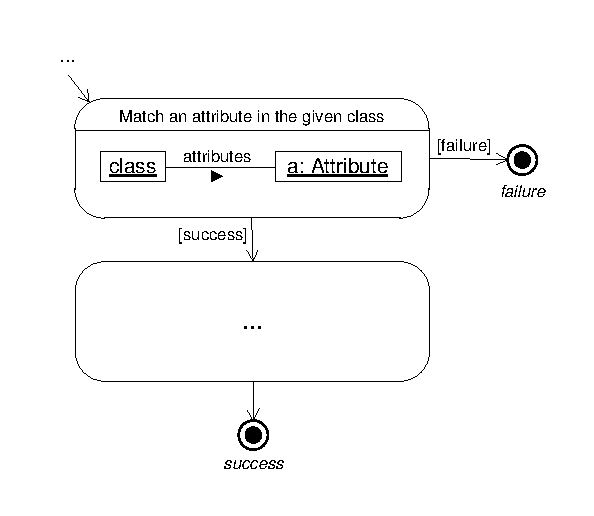
\includegraphics[width=0.7\textwidth]{figures/SuccessAndFailureStopNodes}
  \caption{Example of a success and a failure final node.}
  \label{fig:successAndFailureStopNodes}
\end{center}
\end{figure}

The upper story node in Figure~\ref{fig:successAndFailureStopNodes} specifies that an attribute of a given class object should be matched.
The failure activity edge leads to a final node also labelled with \emph{failure}.
This indicates that the application of the story diagram went wrong.

If an attribute object can be matched however, the control flow continues via the success activity edge to another story node.
Finally, it reaches a final node labelled with \emph{success}.
This indicates that the story diagram's application is considered to be successful.

While the execution of a story diagram is aborted upon reaching a failure final node, the effects of the execution up to this point are not reversed.
All modifications, e.g., object creations and deletions persist.
The developer of a story diagram has to keep this in mind when specifying a transformation.
If these side effects of failed story diagram applications are undesired, the story diagram has to be designed such that it is only aborted if no modifications already took place.
Another way would be to explicitly specify activity nodes which undo the modifications before going to the failure final node.

\todomvd{We could think about a rollback mechanism for later versions.}

\todomvd{Write something about the technical side of the propagation?}
\todoall{Modify metamodel accordingly.}

\subsection{Decision Nodes, Guards, and Loops}
\label{sec:DecisionNodesEtc}

The behavior of a story node is defined by its story pattern.
Therefore,
since trying to find a subgraph defined by a story pattern can fail,
each execution of a story node can also fail.
\tododt{Where is the meaning of failure described exactly? Should it be here or in the story patterns section?
Does success of a story pattern execution mean that there was a successful matching only, independly of the succeeding transformations,
or does it mean that the graph transformation (if available) could also be executed (was executable without contradictions, exceptions not considered)?
I think, success should include the transformation and we should, if possible, check
if a modifying story pattern can perform its modifications after a successful matching \emph{before} actually modifying the host graph
(check if all variables are matched and if there are contradictions).
Someone has to describe that in the story patterns section or here.}

To distinguish the cases of a successful story node execution and its failure,
the outgoing activity edges can be provided with the guards \fe{\text[success\text]} and \fe{\text[failure\text]} (see Figure~\ref{fig:SD-decisions} a)).
The control flow is following the activity edge with the \emph{success} guard in case of a successful story node execution,
i.e.\ a successful matching of the corresponding story pattern.
Otherwise it follows the activity edge with the \emph{failure} guard.
If an outgoing activity edge has no guard, it covers both cases, success and failure.
The guards \fe{\text[success\text]} and \fe{\text[failure\text]} can only be used pair-wise (exactly two outgoing activity edges with exactly these two guards).
The first story node in Figure~\ref{fig:simpleStoryDiagram} (p.~\pageref{fig:simpleStoryDiagram}), for example, uses these guards.

\begin{figure}[htb]
	\centering
  \begin{minipage}[t]{.5\textwidth}
    \centering
    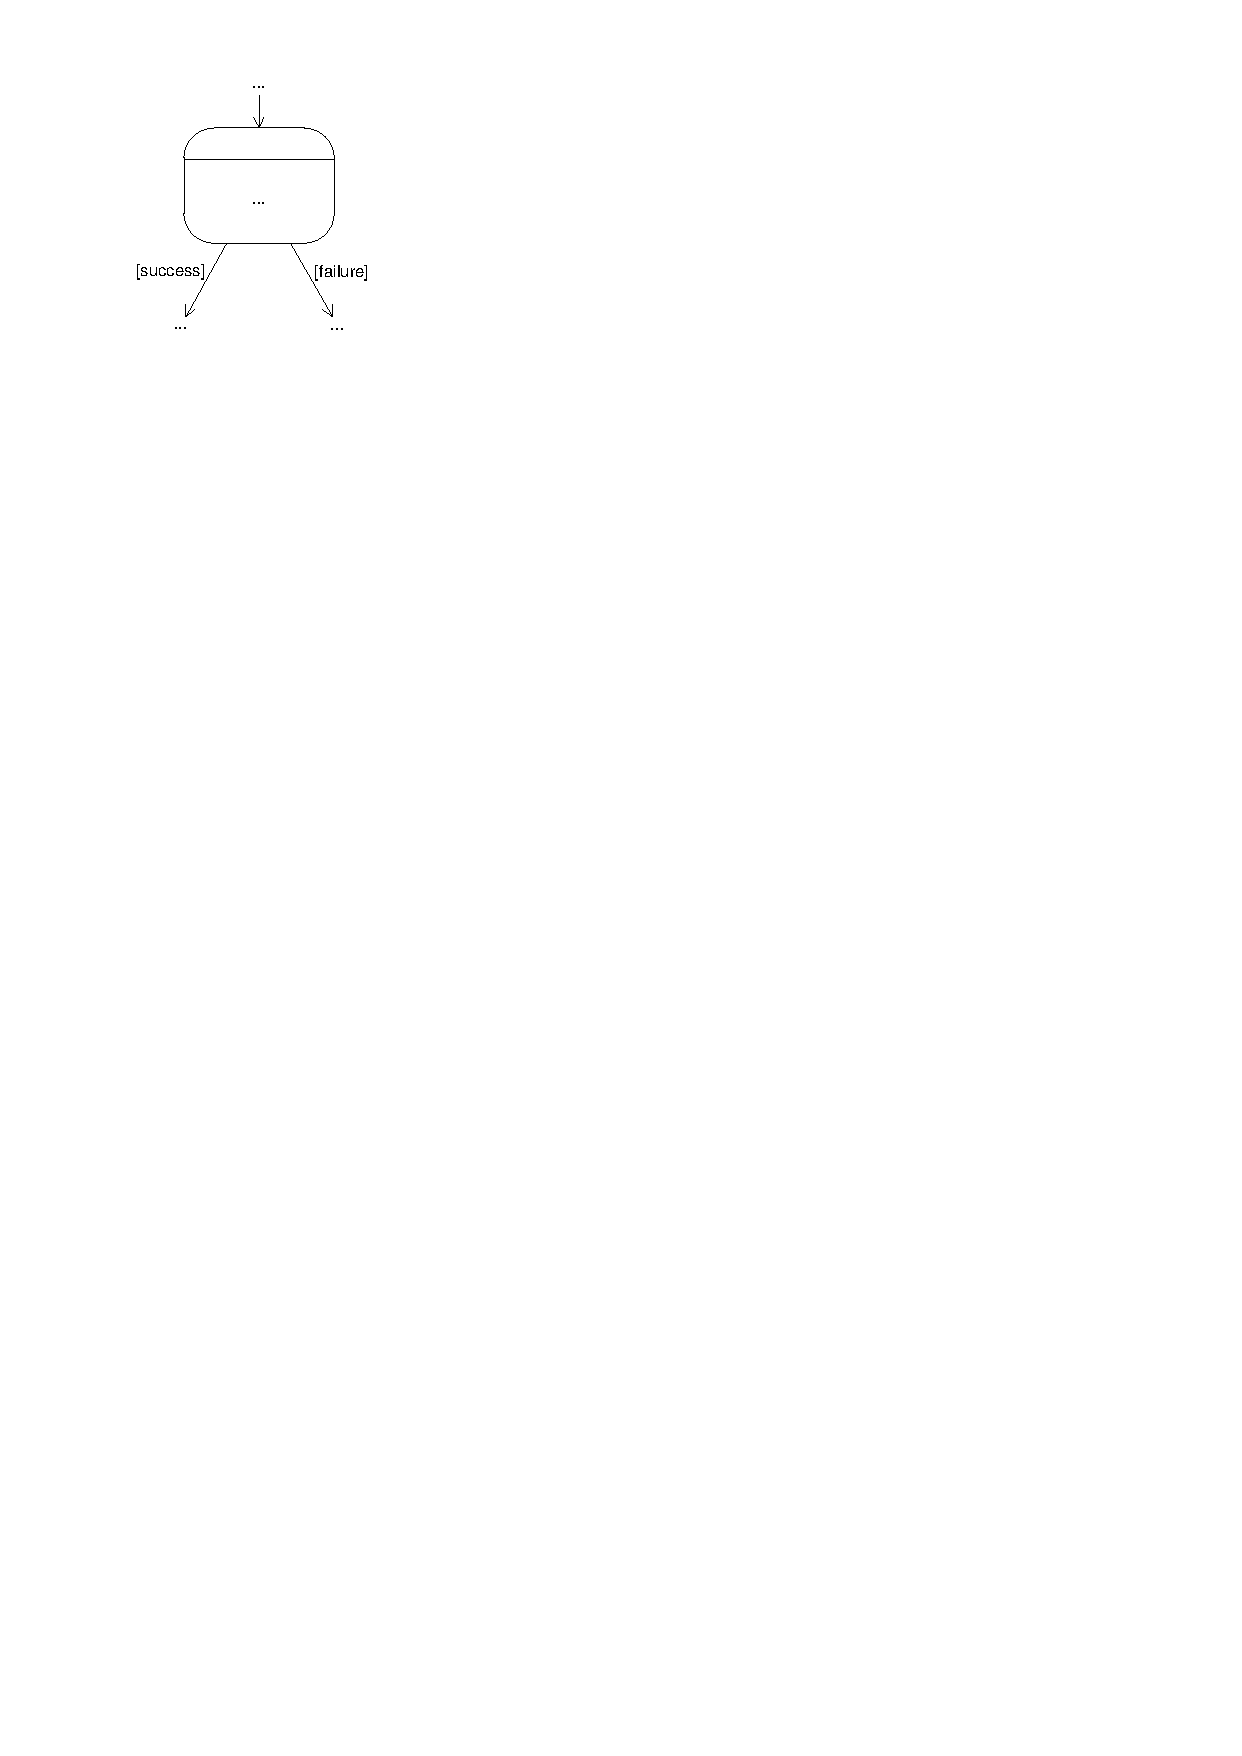
\includegraphics[scale=1]{SD-decision1}
    \\a)
    %\caption{a) Matching-Dependent Decision}
    %\label{fig:SD-decision-success}
  \end{minipage}%
  \hfill
  \begin{minipage}[t]{.5\textwidth}
    \centering
    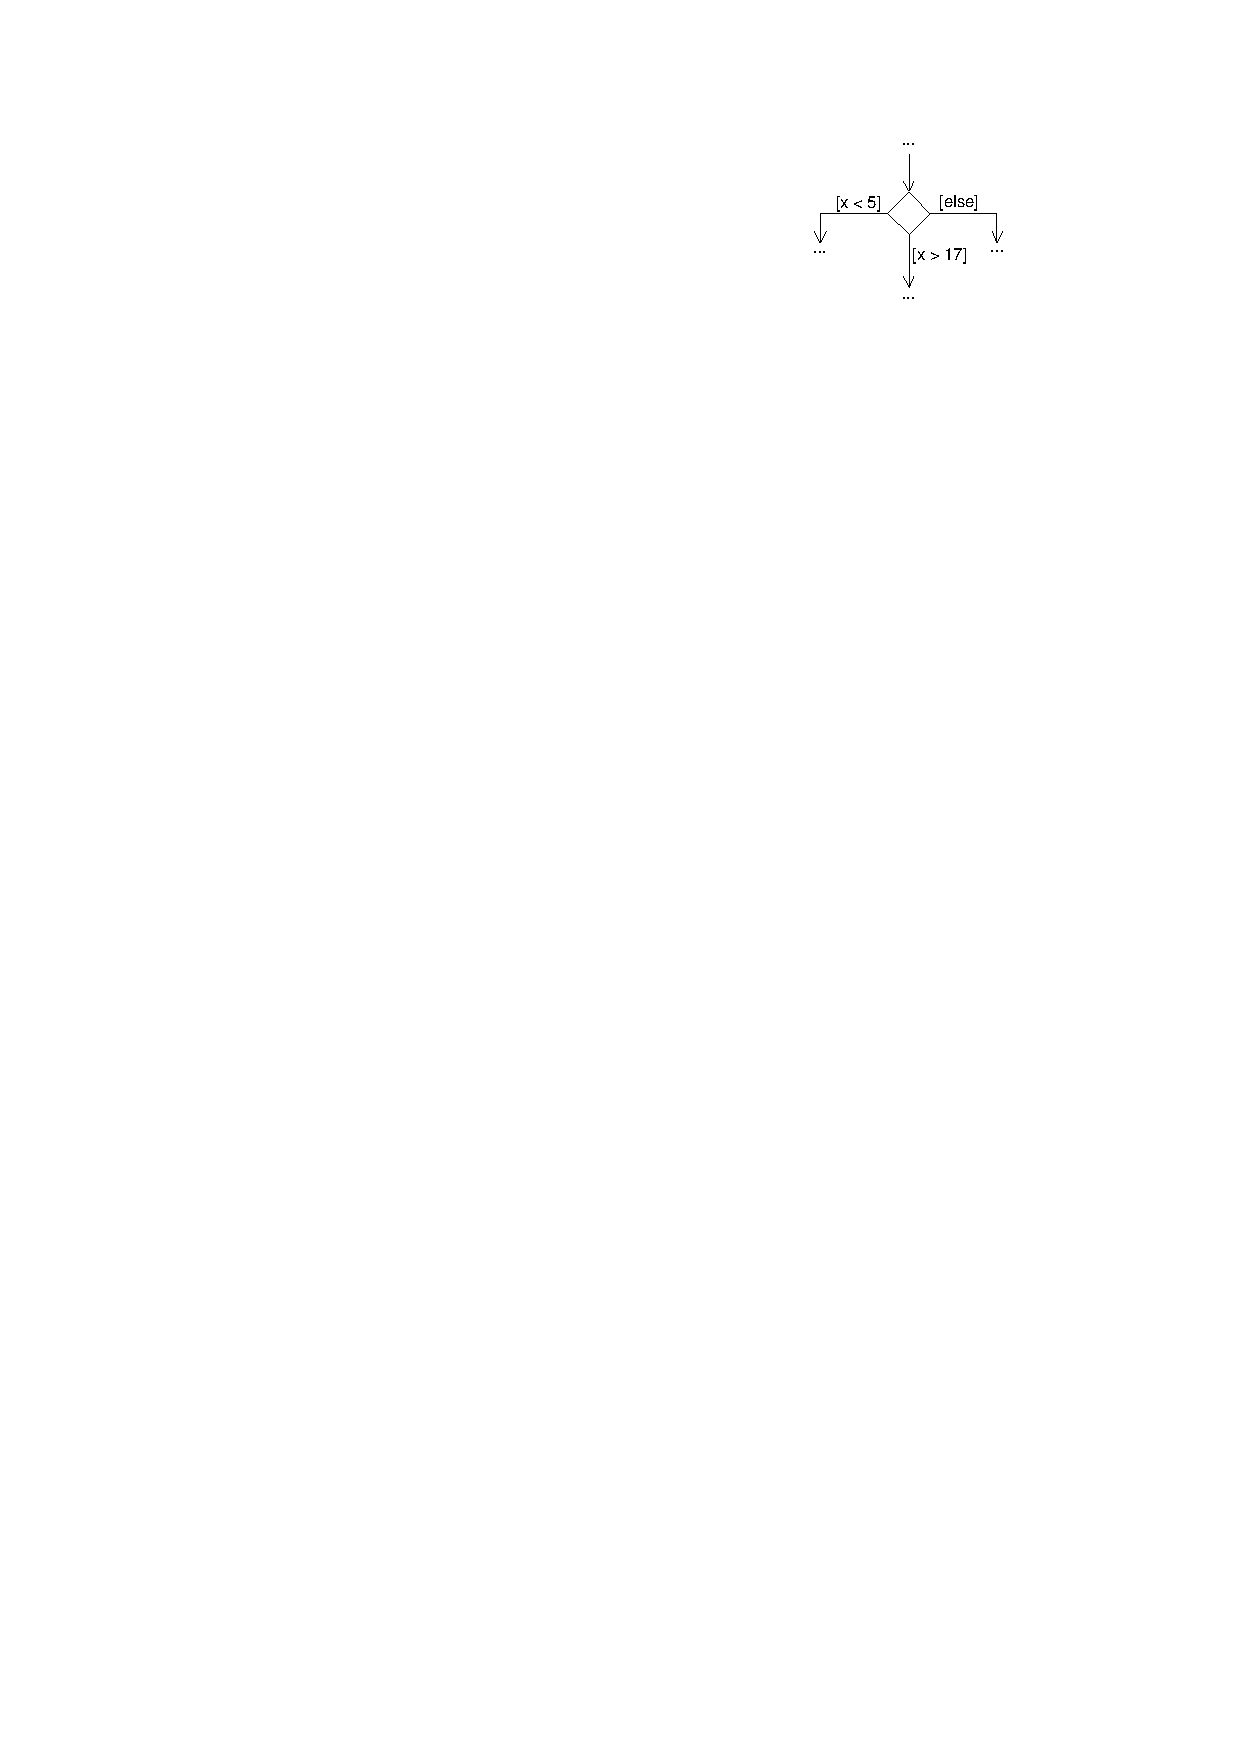
\includegraphics[scale=1]{SD-decision3}
    \\b)
    %\caption{b) Decision Node}
    %\label{fig:SD-decision-boolean}
  \end{minipage}
%  \hfill
%  \begin{minipage}[t]{.3\textwidth}
%    \centering
%    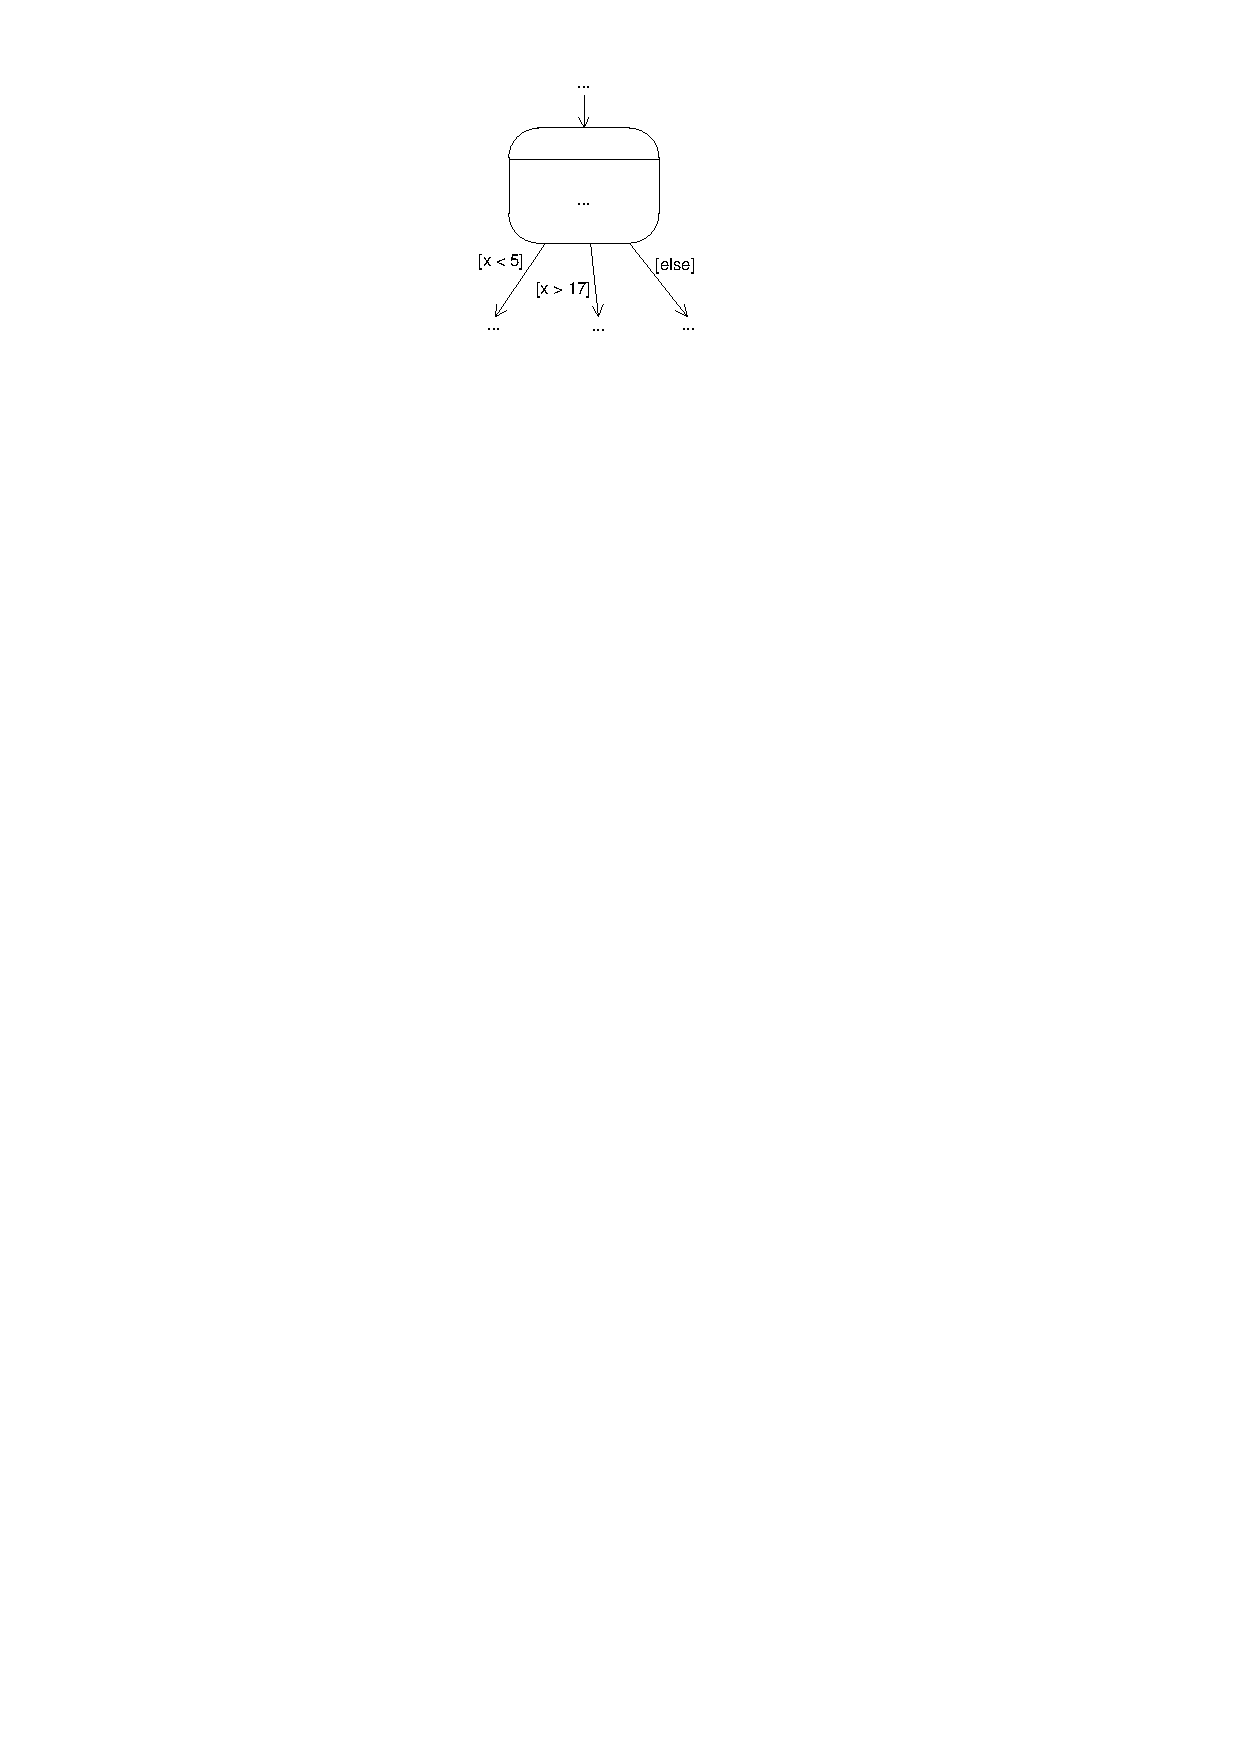
\includegraphics[scale=1]{SD-decision2}
%    \\c)
%    %\caption{c) Boolean Conditions}
%    %\label{fig:SD-decision-nodes}
%  \end{minipage}
  \caption{Examples For Decisions}
  \label{fig:SD-decisions}
\end{figure}

Besides \fe{\text[success\text]} and \fe{\text[failure\text]}, boolean expressions can be used as guards (see Figure~\ref{fig:SD-decisions} b)).
We use the \emph{junction node} -- depicted as a diamond -- for decisions that do not depend on a previous story node.
In this case, the boolean expression of the outgoing activity edge is evaluated to \emph{true} or \emph{false}.
There can be arbitrarily many outgoing activity edges with boolean guard expressions.
The boolean expressions have to mutually exclude each other
and the corresponding guards have to be combined with an outgoing activity edge with the guard \fe{\text[else\text]}.
I.e., if there is a guard with a boolean expression, there is also an activity edge with the guard \fe{\text[else\text]}.

\begin{figure}[htb]
	\centering
  \begin{minipage}[t]{.24\textwidth}
    \centering
    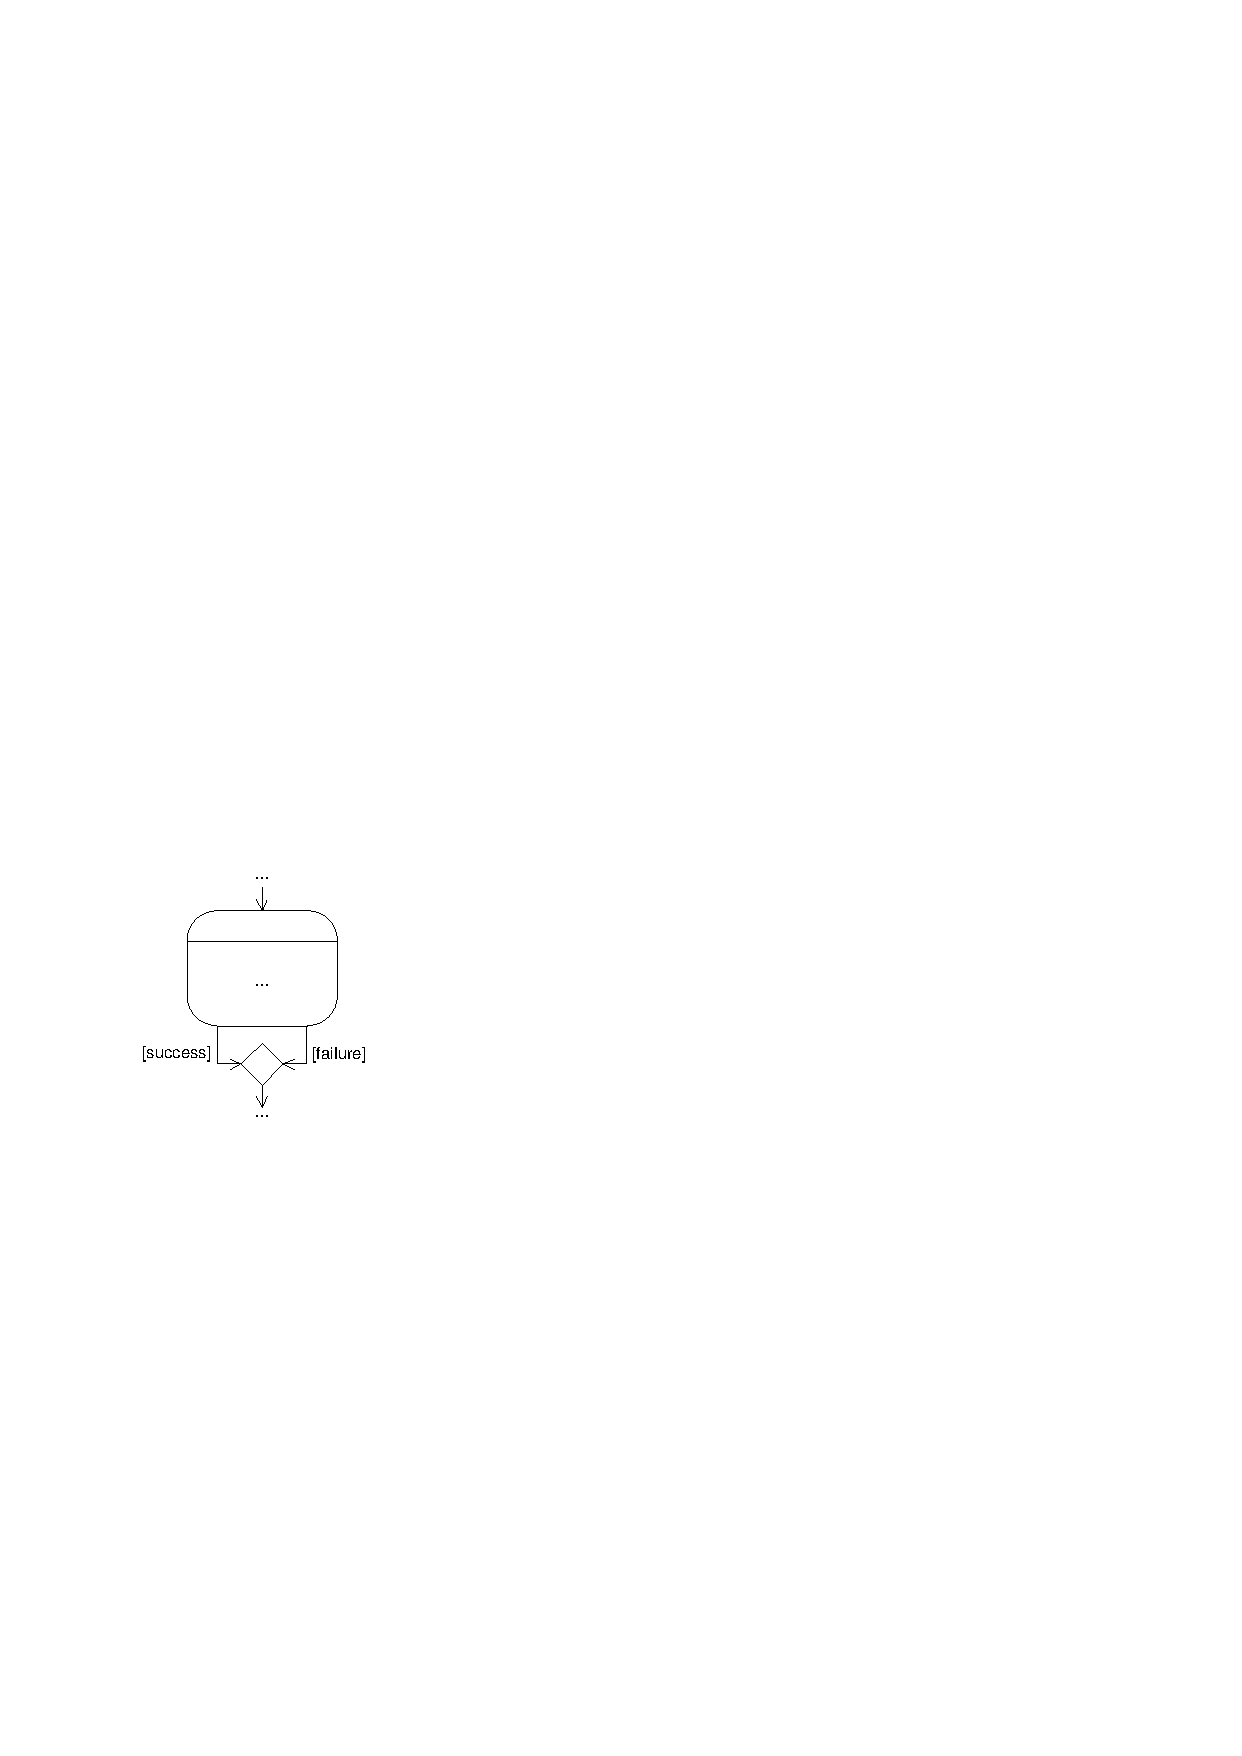
\includegraphics[scale=0.9]{SD-simplify1a} 
    \\a)
    %\caption{a) Each-Time Loop}
    %\label{fig:SD-loop-for-each}
  \end{minipage}%
  \hfill
  \begin{minipage}[t]{.24\textwidth}
    \centering
    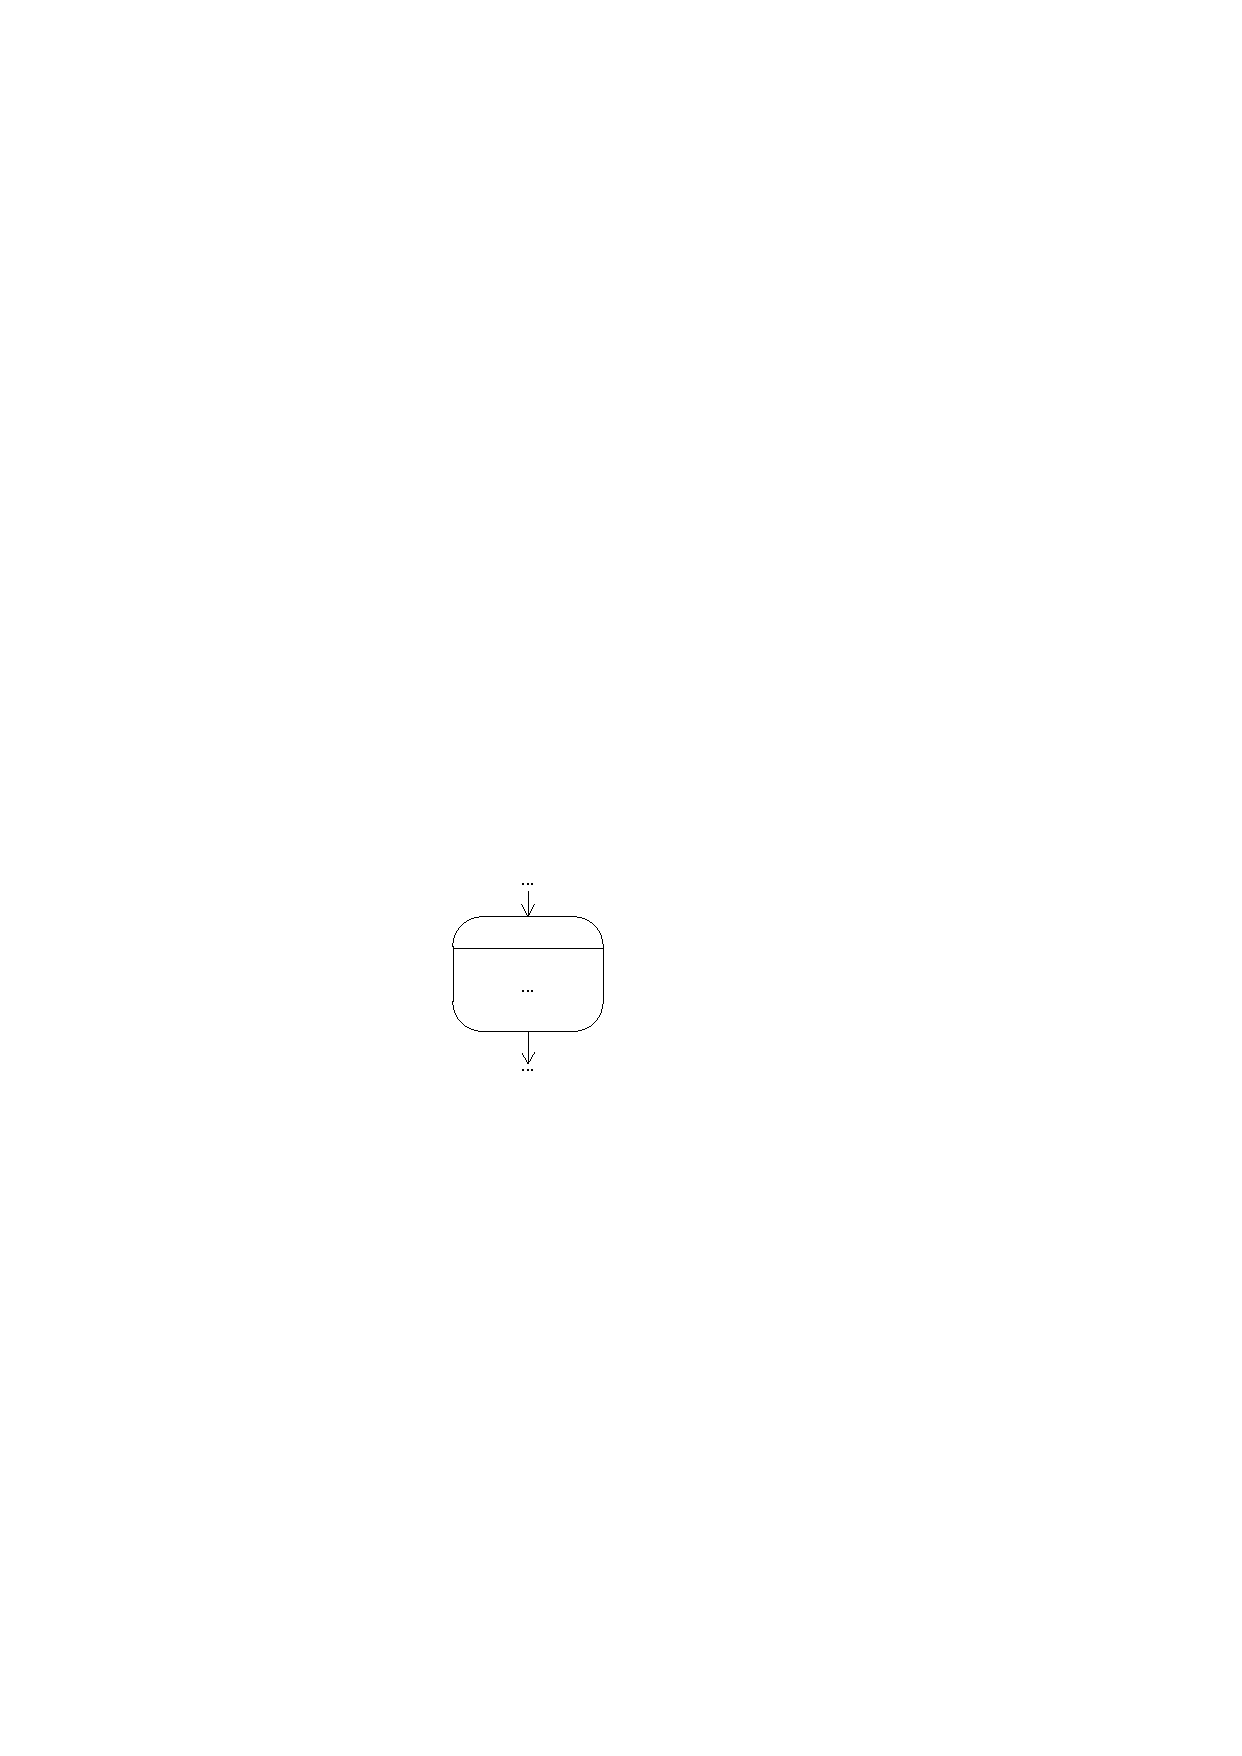
\includegraphics[scale=0.9]{SD-simplify1b}
    \\b)
    %\caption{b) Matching-Dependent Loop}
    %\label{fig:SD-loop-matching}
  \end{minipage}
  \hfill
  \begin{minipage}[t]{.24\textwidth}
    \centering
    \includegraphics[scale=0.9]{SD-simplify2a}
    \\c)
    %\caption{c) Boolean-Condition Loop}
    %\label{fig:SD-loop-boolean}
  \end{minipage}
  \hfill
  \begin{minipage}[t]{.24\textwidth}
    \centering
    \includegraphics[scale=0.9]{SD-simplify2b}
    \\d)
    %\caption{c) Boolean-Condition Loop}
    %\label{fig:SD-loop-boolean}
  \end{minipage}
  \caption[Examples For Control Flow Simplifications]{Examples For Control Flow Simplifications: case a) is semantically equivalent to b), case c) is semantically equivalent to d)}
  \label{fig:SD-simplifications}
\end{figure}

The junction node can also be used to merge several control flows into one
(several activity edges point to a junction node which has only one outgoing activity edge,
see Figure~\ref{fig:SD-simplifications} a)).

In order to simplify the control flow as shown in Figures~\ref{fig:SD-simplifications} a) and c),
we also allow shorthand notations as illustrated in Figures~\ref{fig:SD-simplifications} b) and d).
The control flow in case b) is semantically equivalent to that in case a).
The control flows in cases c) and d) are also equivalent.

\begin{figure}[htb]
	\centering
  \begin{minipage}[t]{.3\textwidth}
    \centering
    \includegraphics[scale=1]{SD-loop1} 
    \\a)
    %\caption{a) Each-Time Loop}
    %\label{fig:SD-loop-for-each}
  \end{minipage}%
  \hfill
  \begin{minipage}[t]{.3\textwidth}
    \centering
    \includegraphics[scale=1]{SD-loop2}
    \\b)
    %\caption{b) Matching-Dependent Loop}
    %\label{fig:SD-loop-matching}
  \end{minipage}
  \hfill
  \begin{minipage}[t]{.3\textwidth}
    \centering
    \includegraphics[scale=1]{SD-loop3}
    \\c)
    %\caption{c) Boolean-Condition Loop}
    %\label{fig:SD-loop-boolean}
  \end{minipage}
  \caption{Examples For Loops}
  \label{fig:SD-loops}
\end{figure}

Activity edges and guards can be used to model loops as illustrated in Figures~\ref{fig:SD-loops} a) and b).
There is an additional construct to model loops which allows to perform the same operations with each occurrence of a certain object structure.
For that purpose, we use a special activity node that we call \emph{for-each} activity node
and special guards \fe{\text[each time\text]} and \fe{\text[end\text]}.

The for-each activity node is depicted by a cascaded activity node (see Figure~\ref{fig:SD-loops} c)).
The second activity node in Figure~\ref{fig:simpleStoryDiagram} (p.~\pageref{fig:simpleStoryDiagram}), for example, is a for-each activity node.
Such a node represents a loop where the contained story pattern is executed as often as new subgraphs can be matched
that differ from the previously matched graphs by at least one other matched object.
The story pattern in the for-each activity node in Figure~\ref{fig:simpleStoryDiagram}
is matched for each existing pair of a method (object variable \fe{anyMethod}) and corresponding call object (object variable \fe{c}).
Besides the matching itself, all \emph{destroy} and \emph{create} steps are also executed for each of these matched subgraphs.
In general, after execution of the story pattern in the for-each activity node,
the control flow follows the activity edge with the guard \fe{\text[each time\text]}, if available (see Figure~\ref{fig:SD-loops} c)).
This edge is optional and can be omitted like in Figure~\ref{fig:simpleStoryDiagram}.
The \fe{[each time]} edge leads to the activity node (or a sequence of such nodes)
that is to be executed after each successful execution of the for-each activity node.
After that, the control flow returns to the for-each activity node in order to match and process the next object structure that can be matched by the for-each activity node.
If there is an activity edge with the guard \fe{\text[each time\text]}, there has also to be such an activity edge leading back to the for-each activity node.
This constitutes a loop.
Finally, the control flow is guided by the activity edge with the guard \fe{\text[end\text]} which leads to the activity node to be executed after the loop.
Each for-each activity node must have such an outgoing \text[end\text] activity edge.

\todojr{fresh matches, auch fuer maybe\_bound: Behaelt ein maybe\_bound-Knoten ein Binding, was erst im Loop gesetzt wurde? Oder zaehlt dafuer nur, was vor dem Loop schon gebunden war? Letzteres erscheint sinnvoller (Stephan fragen wegen Beispiel)}

\subsection{Propagation of Matchings}
\label{sec:storydiagrams:propagation}

The control flow specified by the activity edges determines how matchings of story patterns are propagated through the activity. An initial matching associating objects of the instance model with object variables is established by the input parameters of the activity. In a story pattern inside a story node, we refer to matched objects by using bound variables. Then, the story pattern inside a story node is matched. If the matching process was successful, the matching is extended by the objects which were newly matched by the story pattern and is propagated via the \emph{success} activity edge to the next activity node. If the matching process was not successful, the matching is not changed and the original matching which was passed to the activity node is propagated along the \emph{failure} activity edge.

In case of a loop, the matching which is propagated into the for-each activity node is extended by the matching of the story pattern which is contained in this activity. If the matching is successful, the extended matching is propagated along the \emph{each time} activity edge. After the control flow returns to the for-each activity node, the matching is reset to the matching that originally entered the for-each activity node. As a consequence, in any case the matching which is propagated into the for-each activity node is propagated down the \emph{end} activity edge. Objects and links created throughout the loop, however, remain in instance model.

\todoch{Do you all agree with that semantics? Jan and I do ;-).}
\tododt{I disagree with the matching propagation in loops.
I would like to allow objects matched in a loop iteration to be reused in the next iteration (e.g.\ for moving a pointer in a list during a search).
To be more precise, I would like that the matching for all variables passed to the for-each node is updated during loop iteration and is available in the next iteration.
The same variables with their latest values should be passed through the end activity edge.
During a single loop iteration, the matching is extended by variables newly declared in the loop,
but these are not visible in the next loop iteration and should not be passed through the end activity edge.
This would comply with local variables in the scope of a loop in Java which are not visible outside the loop or in the next loop iteration
if they were not already declared previous to the loop.
For example in Figure~\ref{fig:propagation},
\fe{p1} and \fe{p2} are declared previous to the for-each activity node.
Thus, they are passed to the for-each node, their matchings are updated during the loop iterations, passed through all loop iterations
and eventually passed with their latest matchings through the end activity edge.
In contrast, the object variable \fe{c} is not passed through the end activity edge,
since it was not available previous to the loop, i.e.\ not passed to the for-each activity node.
I would also allow to overwrite the matching that is passed to the for-each activity node and thus allow to match a new object, e.g.\ to the object variable \fe{p1}.
I also talked about this with Jan and we agreed.}

\begin{figure}[htbp]
\begin{center}
  \includegraphics[width=0.8\textwidth]{figures/PropagationOfMatchingsExample}
  \caption{Propagation of Matchings through a Story Diagram}
  \label{fig:propagation}
\end{center}
\end{figure}

Figure~\ref{fig:propagation} gives an example for the propagation of matchings. The initial matching consists of two objects of type \fe{Package} which are bound to the input parameters \fe{p1} and \fe{p2}. This matching is passed to the for-each activity node \fe{A}. In this activity, the story pattern tries to match a class in the package bound to \fe{c1}. For each class that is found, the matching is extending by the corresponding class and propagated along the \emph{each time} activity edge to the activity node \fe{B}. In \fe{B}, the object variable \fe{c} is unbound. Thus, a new matching for \fe{c} is to be obtained. If the story pattern is matched successfully, the matching that is propagated down the activity edge to \fe{C} consists of the two packages as well as a class contained in the package bound to \fe{p2}. If the story pattern in \fe{B} cannot be matched, then the matching is propagated unchanged. Then the matching in \fe{C} contains the two packages as well as a class which is contained in the package bound to \fe{p1}. If the control flow reaches the for-each activity node \fe{A} again, then the matching is reduced to the two packages bound to \fe{p1} and \fe{p2}. If the for-each activity node \fe{A} is left via the \emph{end} activity edge, exactly that matching is propagated.

If the control flow reaches a final node, only objects that are contained in the matching which is propagated to the final node may be returned. The use of decision nodes in combination with activity edges having a boolean guard does not change the propagation of matchings. The boolean condition at the edge only defines where the matching is propagated.

\subsection{Story Diagram Calls}
\label{sec:Calls}
Story diagram calls are special nodes in a story diagram which are used to invoke other story diagrams. Similar to method calls, this reduces redundancy and promotes reuse.

As described in Section~\ref{sec:activities}, a story diagram can have an arbitrary number of in and out parameters. When calling a story diagram, concrete arguments have to be assigned to the in parameters. Consequently, if an object variable named \fe{n} is bound somewhere in the story diagram, the identifier \fe{n} can be used to pass this object variable as an argument to a call. If the called story diagram has out parameters, those are bound explicitly by assignments at the stop activity node. They can be used in the calling story diagram by specifying object variables whose names match those of the out parameters.

For in parameters, we use a call-by-reference semantics. If an object that is passed as an in parameter is modified in the called story diagram, those modifications remain after the called story diagram has terminated. The object in question can be used in the calling story diagram after the call but the call may have modified its attributes or its links.

An example of a story diagram call is shown in Figure~\ref{fig:call}.

\begin{figure}[htb]
\begin{center}
  \includegraphics[width=\textwidth]{figures/StoryDiagramCall}
  \caption{Example of a story diagram call}
  \label{fig:call}
\end{center}
\end{figure}

The first story pattern in Figure~\ref{fig:call} shows the bound object variable \fe{package}. Two new object variables \fe{class1} and \fe{class2} are bound in that pattern. The next node with the grey background is a story diagram call which is also signified by its label \fe{Call}. Beneath the label, the name of the called story diagram is given, in this case \fe{CreateBidirectionalAssociation}. Assume that the called story diagram has two in parameters of the type \fe{Class} and one out parameter of the type \fe{Association}. The two classes that were bound in the first story pattern, \fe{class1} and \fe{class2} are passed to the call as arguments. They can be used in the story node after the call without passing the back as out parameters. The modifications carried out by the called story diagram (i.e.\ the creation of the \fe{assoc} object and its connection to \fe{class1} and \fe{class2}) are retained after the call terminates.
The result of the call is bound to the object variable \fe{assoc}. The type of this variable is determined by the out parameter type, i.e., in this case the type Association.

If a story diagram has no out parameters, the keyword \fe{void} follows the colon instead of the out parameter's names (see Figure \ref{fig:SDRemoveInterfaceViolation} for an example).

%Issues for future versions:
% method calls
% polymorphic calls

%\ext
{
\subsection{Exception Handling}
}




	\section{Expressions (Dietrich)} \label{sec:Expressions}

Story diagrams and story patterns use a mainly graphical syntax.
Though, some things can compactly be described by text, e.g., restrictions of attribute values to a certain range.
For this purpose we added a small textual language for expressions to story diagrams
to cover value comparisons, value assignments, simple arithmetic expressions, etc.
In this first version of this technical report we do not describe expressions in detail.

Besides our small textual language for certain expressions, we support embedding OCL expressions, for example, to determine a value to be assigned to an attribute\footnote{Currently,
the OCL tools in Eclipse (\href{http://www.eclipse.org/modeling/mdt/?project=ocl}{http://www.eclipse.org/modeling/mdt/?project=ocl}),
as far as possible, comply with the OMG OCL standard 2.3 (\href{http://www.omg.org/spec/OCL/2.3/Beta2/PDF}{http://www.omg.org/spec/OCL/2.3/Beta2/PDF}).
We use these tools to interpret the OCL expressions.
More details about this issue can be found here:\\ \href{http://www.eclipse.org/projects/project-plan.php?planurl=http://www.eclipse.org/modeling/mdt/ocl/project-info/plan_indigo.xml&component=Eclipse}{http://www.eclipse.org/projects/project-plan.php?planurl=http://www.eclipse.org/modeling/mdt/ocl/project-info/plan\_indigo.xml\&component=Eclipse}}.
In future, this will be extended to also cover arbitrary other textual expressions that have to be interpreted by a given interpreter.
	
	\section{Templates (Dietrich)}
	
	\section{Previous Work (Jan)}

\todomvd{This ``Short history of Fujaba'' seems odd here. Maybe we should it put at the end of the introduction?}

Story diagrams have been described first by Fischer et al. \cite{FNTZ00} and Jahnke and Z\"{u}ndorf \cite{JZ98} in 1998.
The foundations of story diagrams lay in the programmed graph rewriting systems PROGRES \cite{SWZ95} which has been developed at the University of Aachen since 1989.
Story diagrams (or story flow diagrams, as they have been called in early publications) adapt and enhance the PROGRES approach to a UML-like notation and an object-oriented data model \cite{JZ98}, using an easily comprehensible graphical syntax and well-defined semantics.
Z\"{u}ndorf \cite{Zun01} describes the syntax and semantics of early story diagrams in detail.
A graph grammar that formally describes the syntax of the control flow of story diagrams was defined by Klein \cite{Kle99}.
Story diagrams are embedded in a rigorous and systematic software development method called story driven modeling \cite{Zun01,DGZ04}.

From the beginning, there was strong tool support for story diagrams.
In December 1997 the Fujaba project started at the University of Paderborn.
A first prototype was implemented in the course of a master thesis \cite{FNT98}.
Fujaba, an acronym for ``From UML to Java And Back Again''\footnote{The acronym is derived from a preceding tool called FUCABA (''From UML to C++ And Back Again'') \cite{JZ97}.}, combines UML class diagrams, UML activity diagrams, and story diagrams to allow completely specifying the structure and behavior of software systems.
These specifications can then be executed.
For instance, Z\"{u}ndorf, Sch\"{u}rr and Winter \cite{ZSW99} describe how story diagrams can be compiled into Java code.
A first public tool demonstration of Fujaba was presented at the ICSE 2000 \cite{NNZ00}, showing advanced class and story diagram modeling facilities as well as graphical debugging and simulation.

In the following, story diagrams and Fujaba have been modified and enhanced.
Originally, story diagrams use expressions of the target programming language to define constraints, return values etc.
I.e., if a story diagram should be compiled into Java code, Java expressions must be used.
St\"{o}lzel, Zschaler and Geiger \cite{SZG07} integrated OCL into story diagrams, making them more platform-independent.
They conntected Fujaba with the Dresden OCL toolkit, allowing a code generation for story diagrams including the OCL constraints.

SD interpreter \cite{GHS09}

Tichy, Meyer and Giese \cite{TMG06} identified some semantic issues in story diagrams.


%motivation for the acronym Fujaba, \textit{F}rom \textit{U}ML to \textit{J}ava \textit{a}nd \textit{b}ack \textit{a}gain \cite{JZ97}

%story-driven modelling and story boards (roots of Fujaba) \cite{FNT98,FNTZ00,JZ98,ZSW99,DGZ04}

%story diagrams \cite{FNTZ00,Zun01}

%SD graph grammar for the construction of valid SDs (besides others) \cite{Kle99}

%Fujaba tool demo \cite{NNZ00}


%semantic issues \cite{TMG06}

new meta-model \cite{HRvD+11}
